% !TEX root = ../MasterThesis_goto_v1.tex

%%%%%%%%%%%%%%%%%%%%%%%%%%%%%%%%%%%%%%%%%%%%%%%%%%%%%%%%%%%%%%%%%%%%%%%%%%%%%%%%%%%%%%%%%%%%%%%%%%%%%
\chapter{深層学習} \label{chap:DeepLearning}

本章では, 深層学習 (Deep Learning, DL) について述べる。

まず深層学習の導入として, \ref{DL:MachineandDeepLearning}節で機械学習 (Machine Learning, ML) と深層学習の概要について簡単に紹介する。

次に\ref{DL:Perceptron}節では, 深層学習を理解する上で前提となるパーセプトロン (Perceptron) というネットワークを解説する。
パーセプトロンは, 後述するニューラルネットワークの先駆けとなる技術である。

\ref{DL:NeuralNetwork}節では, 深層学習の基礎技術であるニューラルネットワーク (Neural Network, NN) を導入する。
主に, \ref{DL:NN:StructureofNN}項でニューラルネットワークを構築するために必要な計算手順について, \ref{DL:NN:TrainingofNN}項でニューラルネットワークの学習に関して重要な技術要素についてそれぞれ説明する。

深層学習は, \ref{DL:NeuralNetwork}節までの基盤的な技術を使用するだけでも様々な問題に対応できるが, 扱うデータや問題の性質によって, 更に応用的な使い方が求められる。
本研究ではそのような応用技術を幾つか用いてネットワークの作成を行なっている。
その為, \ref{DL:RecurrentNeuralNetwork}節や\ref{DL:Attention}節ではそのような深層学習の応用技術の解説を行う。

\ref{DL:RecurrentNeuralNetwork}節では, 系列データを取り扱うためのリカレントニューラルネットワーク (Recurrent Neural Network, RNN) を導入する。
\ref{DL:Attention}節では, 近年注目されている注意機構 (Attention) と呼ばれる技術について説明する。

最後に\ref{DL:HyperParameter}節にて, ニューラルネットワークが持つハイパーパラメータについてまとめる。

本章の作成にあたり, 参考文献\cite{ZeroDeepLearning1, ZeroDeepLearning2, PythonMLPrograming}を使用した。

%%%%%%%%%%%%%%%%%%%%%%%%%%%%%%%%%%%%%%%%%%%%%%%%%%%%%%%%%%%%%%%%%%%%%%%%%%%%%%%%%%%%%%%%%%%%%%%%%%%%%
\section{機械学習と深層学習} \label{DL:MachineandDeepLearning}

深層学習とは, 機械学習の技術の一つである。
本節ではまず, この機械学習について簡単に説明し, その後, 機械学習における深層学習の位置付けを述べる。

機械学習とは, データに現れるパターンや統計情報を計算機 (学習器) に「学習」させることによって, 逐一プログラミングをすることなく未知の問題に対応させる為の技術である。
これは人間の持つ知性を機械に実現する, 人工知能 (Artificial Intelligence, AI) に関する研究の一分野であると言える。
このような研究は, $1956$年のダートマス会議\cite{Dartmouth}から始まり, 現在は第三期のAIブームと言われている。
機械学習は, 機械 (計算機) が独自に未知の問題を解く為の技術や手法の総称であるが, 問題に対するアプローチの仕方によって, 教師あり学習, 教師なし学習, 強化学習などに分類することができる(図\ref{1MachineLearning})。

\begin{itemize}
  \item 教師あり学習\\
  教師あり学習とは, 訓練データ (Training data) と呼ばれる正解がラベル付けされたデータを用い, 学習器の出力を正解に近付けるように学習器を更新していく手法である。
  主にクラス分類を行う分類問題や, 連続値を予測する回帰問題などの問題を解くことができる。
  具体的な例としてサポートベクターマシン (Support Vector Machine, SVM\cite{PatternRecognitionUsingGeneralizedPortraitMethod,TrainingAlgorithmforOptimalMarginClassifiers})や決定木などが挙げられる。
  \item 教師なし学習\\
  教師なし学習とは, 訓練データを用いず, データの持つ数学モデルや構造を抽出する技術である。
  主にクラスタリングや次元圧縮などに使用され, 代表的な手法は, k平均法や主成分分析などである。
  \item 強化学習\\
  強化学習とは, 環境とのやり取りから報酬を受け取り, エージェントを構築していく手法である。
  学習は報酬を最大化するように進み, 教師あり学習の一分野のようにみなす事も出来るが, 強化学習は一連の行動に対しての報酬を考慮する点で異なる。
  強化学習は様々な分野で使用されているが, 主に長期的な戦略が必要となるゲームなどの領域で用いられている。
\end{itemize}

\begin{figure}[htbp]
 \centering
 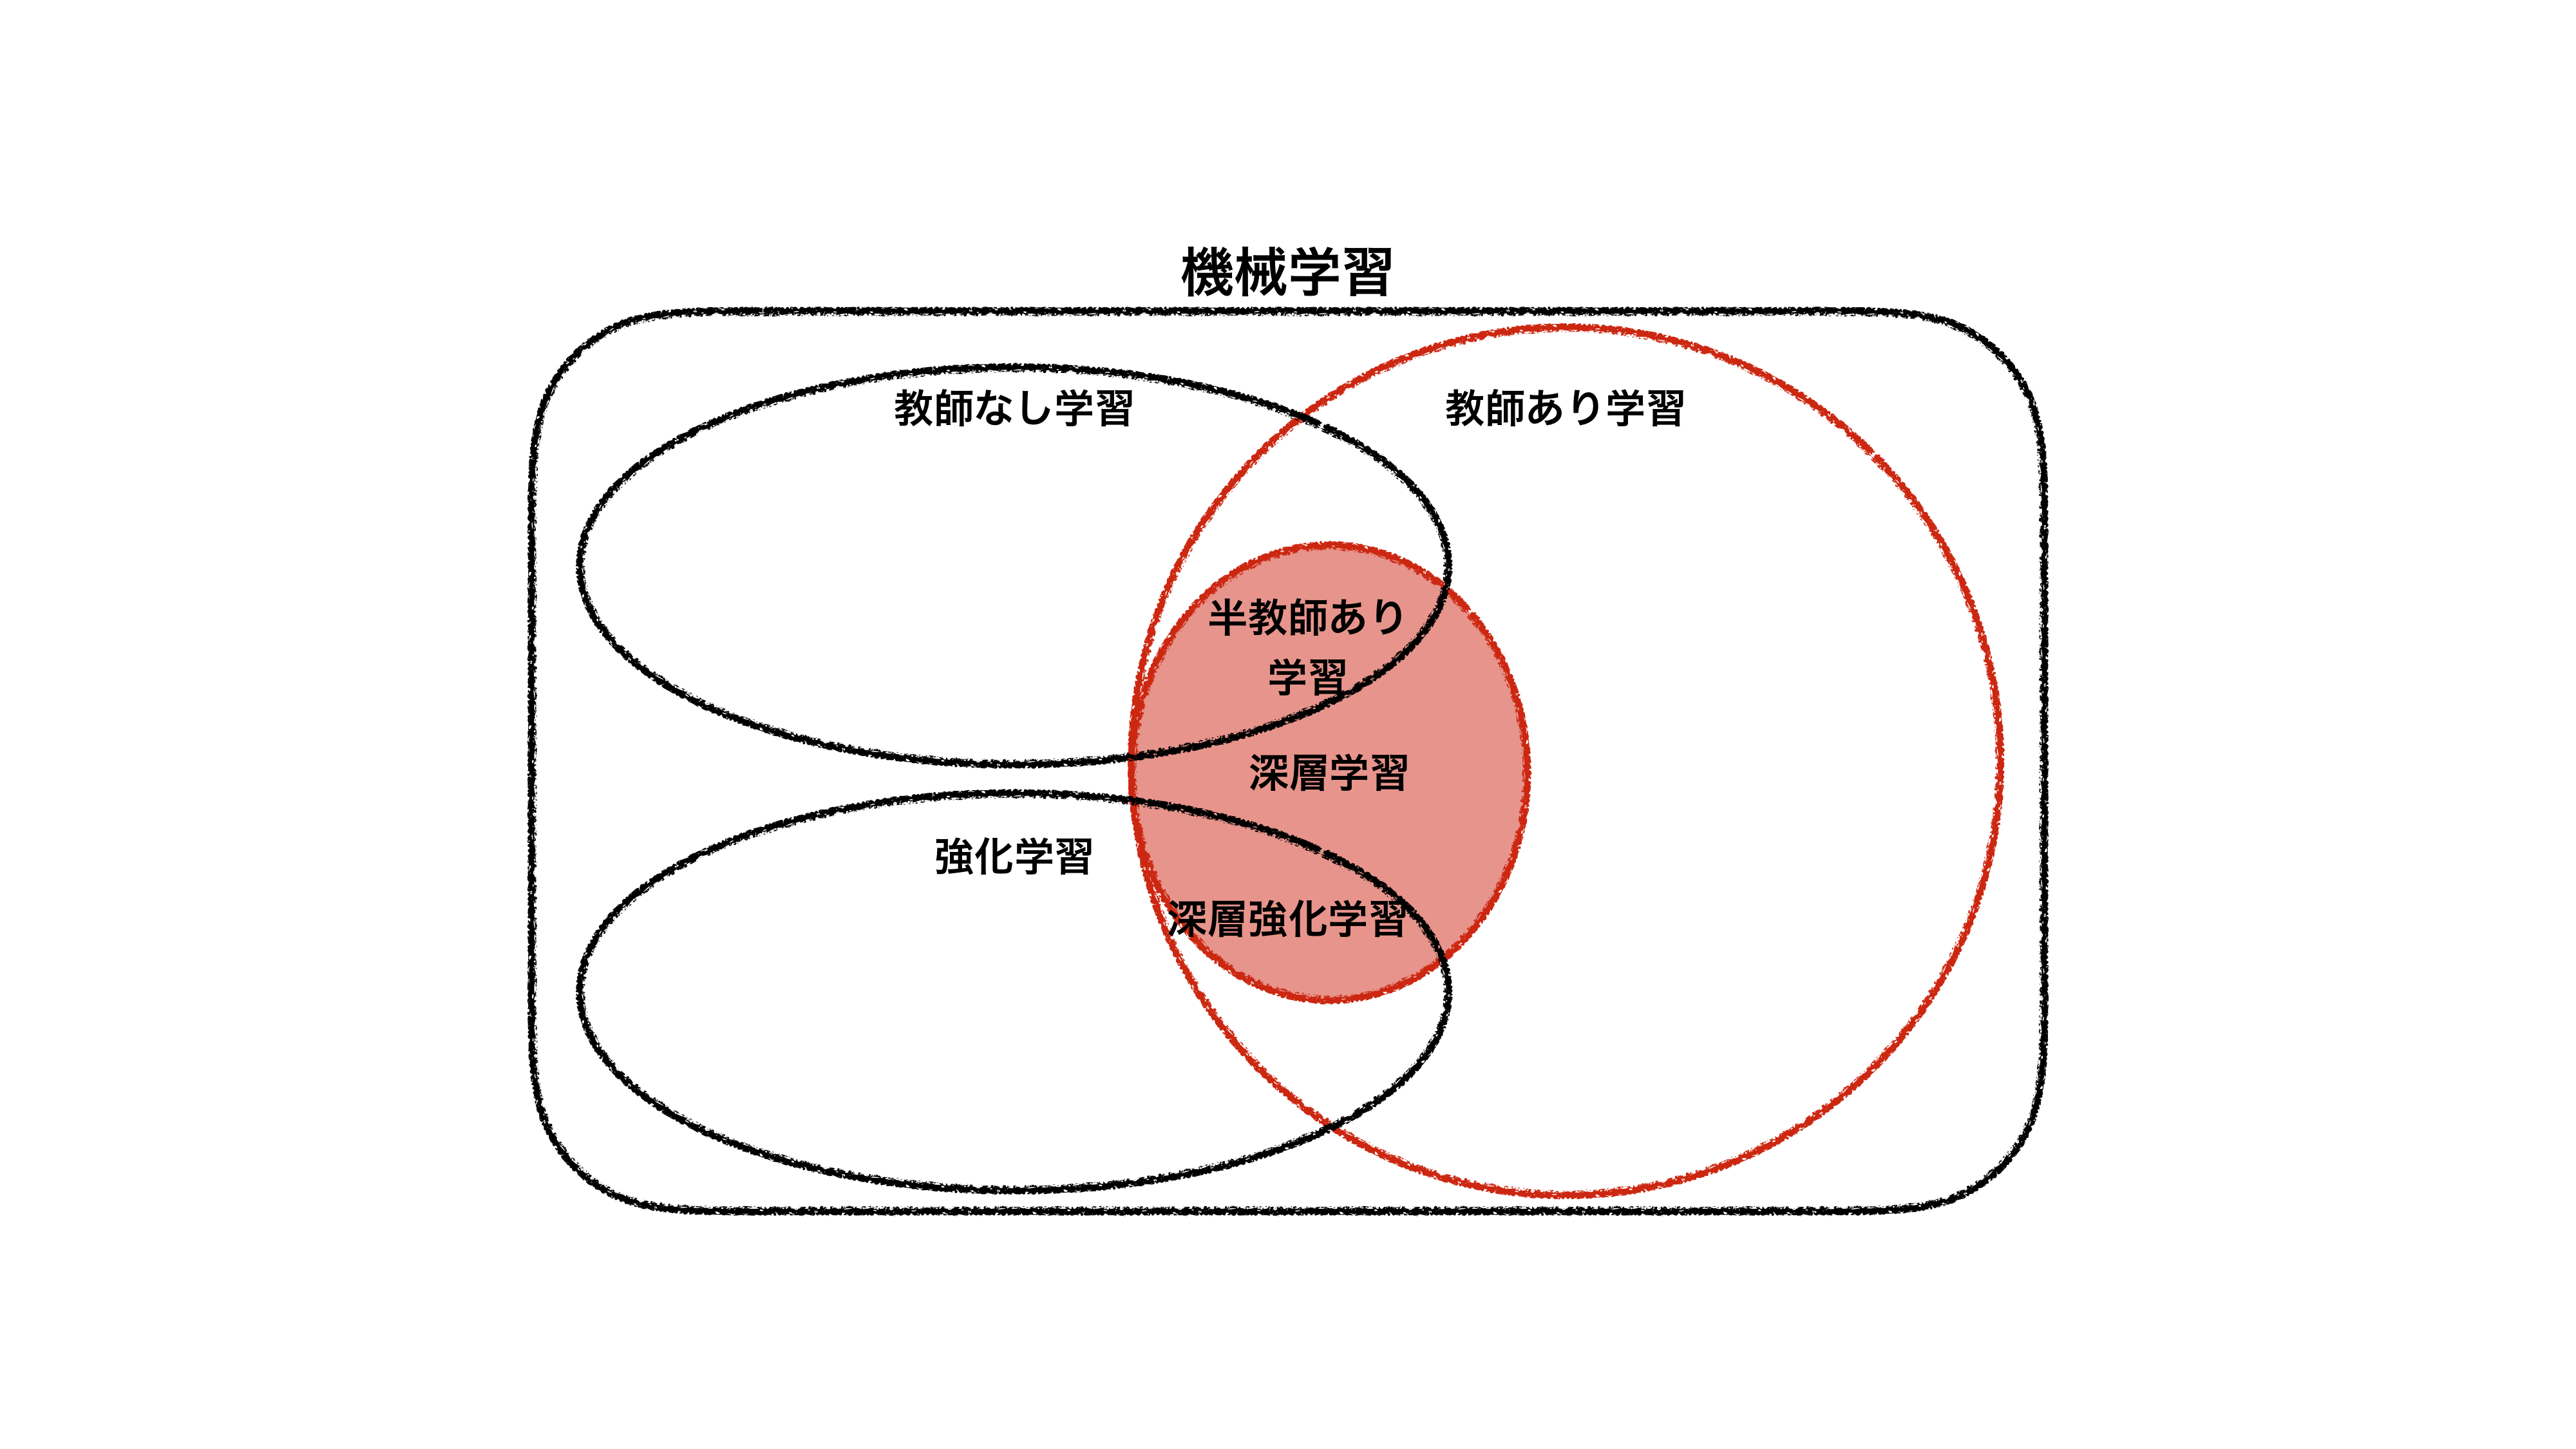
\includegraphics[trim = 0 100 0 50, width=0.9\textwidth, clip]{Figure/2DeepLearning/1MachineLearning.png}
 \caption[機械学習の中の深層学習の位置付け]{機械学習の中の深層学習の位置付け。深層学習は基本的に教師あり学習であるが, 半教師あり学習分類やクラスタリングなど応用的な研究が行われている。}
 \label{1MachineLearning}
\end{figure}

深層学習は, このような機械学習の中で, 基本的には, 回帰問題や分類問題などを解く教師あり学習に分類される。
しかし近年では, 半教師あり学習やディープクラスタリング, 深層強化学習といった様々な技術的応用が提案されている。
次節以降では, この深層学習の基盤技術について紹介する。


%%%%%%%%%%%%%%%%%%%%%%%%%%%%%%%%%%%%%%%%%%%%%%%%%%%%%%%%%%%%%%%%%%%%%%%%%%%%%%%%%%%%%%%%%%%%%%%%%%%%%
\section{パーセプトロン} \label{DL:Perceptron}

パーセプトロンは深層学習の基礎となる技術であり, $1958$年, Rosenblattによって提案された\cite{PerceptronPaper}。
ここでは, このパーセプトロンについて解説することで, 次節のニューラルネットワークへの導入とする。


%%%%%%%%%%%%%%%%%%%%%%%%%%%%%%%%%%%%%%%%%%%%%%%%%%%%%%%%%%%%%%%%%%%%%%%%
\subsection{単純パーセプトロン} \label{DL:Percep:SimplePerceptron}

パーセプトロンとは, 情報を伝達するネットワークである。
ここでのネットワークとは, ある情報を受け取り, それを後方へ伝達するような構造のことを言うものとする。
まず, 最も簡単なパーセプトロンとして, 図\ref{2SimplePerceptron}のような構造を考える。
図\ref{2SimplePerceptron}は, 二つの入力$x_1,x_2$を受け取り, 一つの出力$y$を行なっているネットワークである。
このような入力や出力の数や入力や出力そのものの事をノードやニューロンという。
また, 図\ref{2SimplePerceptron}のように, ただ入力と出力のみを持っているパーセプトロンを特に単純パーセプトロン (Simple Perceptron) という。

\begin{figure}[htbp]
 \centering
 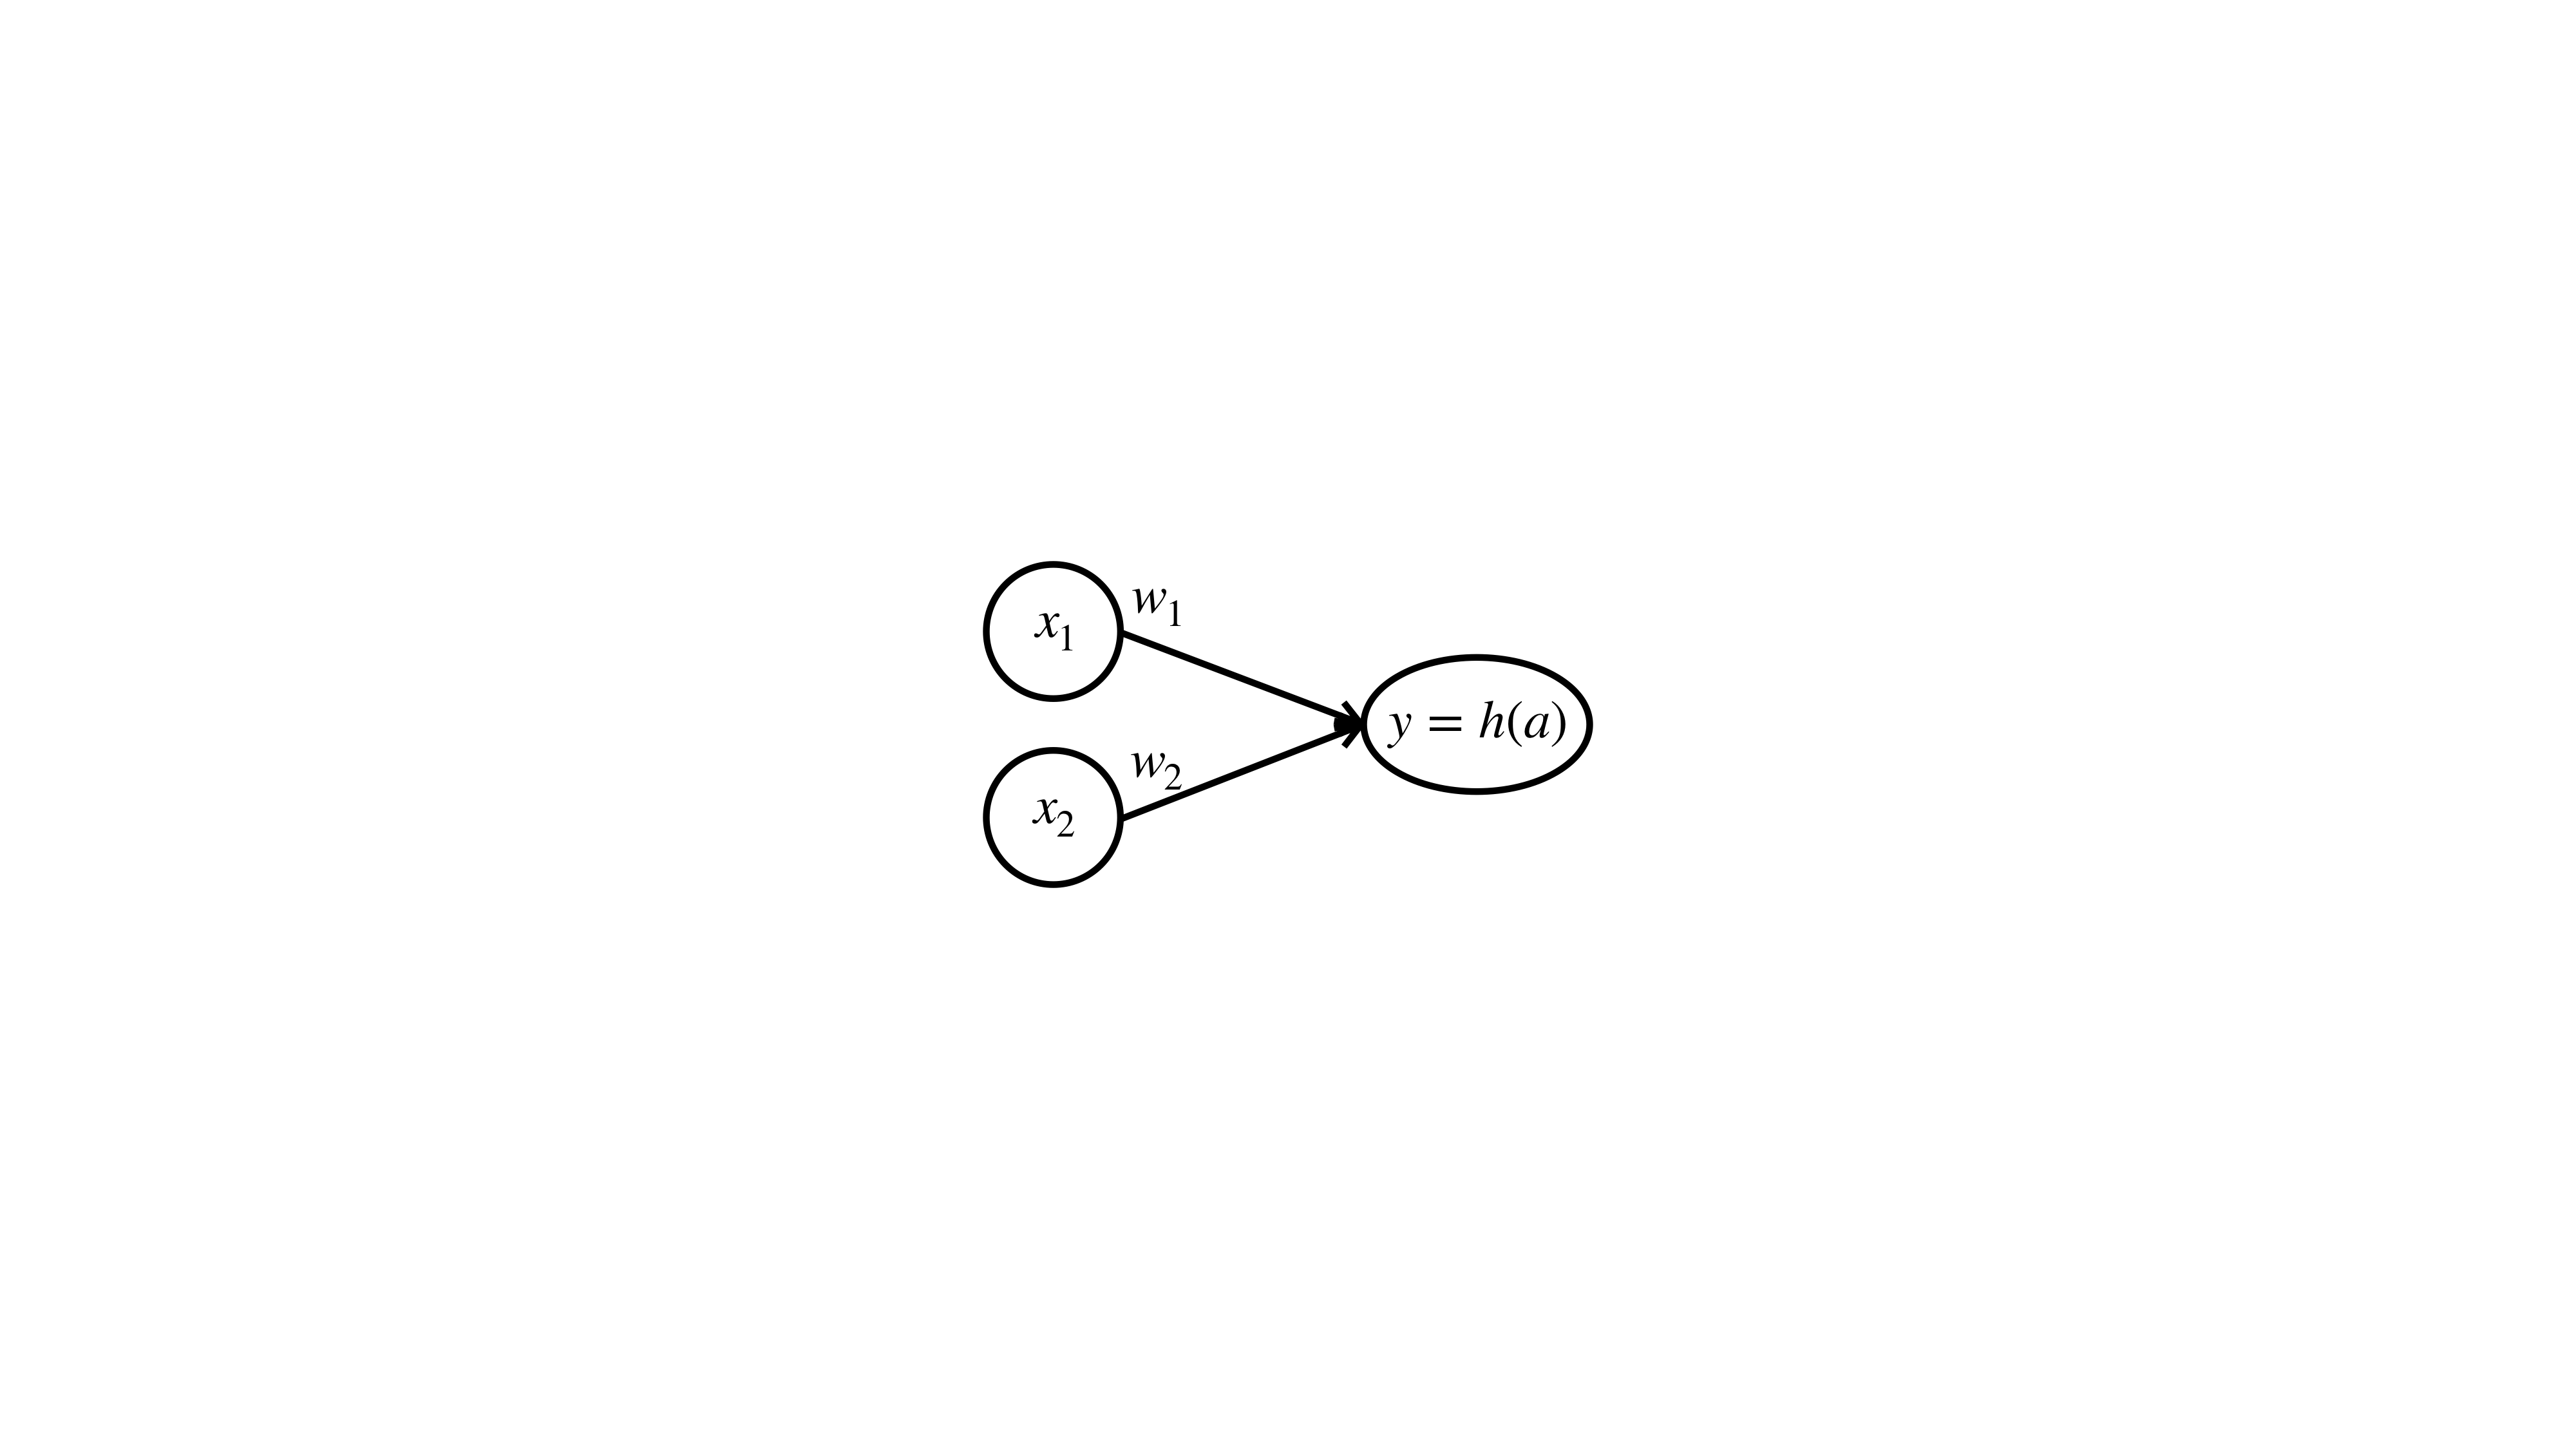
\includegraphics[trim = 250 350 250 350, width=0.9\textwidth, clip]{Figure/2DeepLearning/2SimplePerceptron.png}
 \caption[単純パーセプトロン]{単純パーセプトロン。入力を$x_1,x_2$, 出力を$y$と置いた。また, 各ノードの繋がりを矢印で表現し, 同時にそれぞれの線は学習可能な重みを表している。}
 \label{2SimplePerceptron}
\end{figure}

単純パーセプトロンの情報伝達は, 簡単な計算で定義される。
出力$y$は, $x_1,x_2$とそれぞれの重み$w_1,w_2$を用いて, 
\begin{equation}
 \begin{split}
  y &= h(a)\\
  a &= w_1x_1 + w_2x_2
 \end{split}
\end{equation}
と計算される。
ここで, 出力$y$は関数$h$によって変換されている。
このような関数を活性化関数 (Activation function) という。
特に単純パーセプトロンでは, 活性化関数$h$としてヘヴィサイドの階段関数(図\ref{3HeavisideStepFunction})を用いる。

\begin{figure}[htbp]
 \centering
 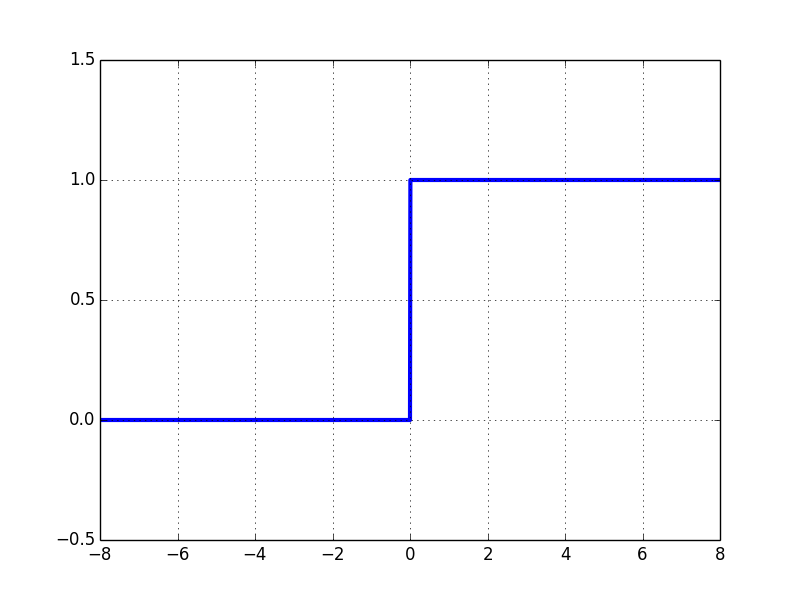
\includegraphics[width=0.5\textwidth]{Figure/2DeepLearning/3HeavisideStepFunction.png}
 \caption{ヘヴィサイドの階段関数}
 \label{3HeavisideStepFunction}
\end{figure}

その閾値を$\theta$とすると, 出力は更に, 
\begin{equation}
 y = h(a) = \left\{ \begin{array}{ll}
    0 & (a = w_1x_1 + w_2x_2 \leqq \theta) \\
    1 & (a = w_1x_1 + w_2x_2 > \theta)
 \end{array} \right.
\end{equation}
と書ける。
この時, 単純パーセプトロンはある一定値$\theta$までは"$0$", それ以上であれば"$1$"を返す二値信号のネットワークであると考えることが出来る。
パーセプトロンやニューラルネットワークにおいて, 学習可能なパラメータは重み$w_1,w_2$であり, これら重みを更新していく操作を学習 (トレーニング, Training) という。


%%%%%%%%%%%%%%%%%%%%%%%%%%%%%%%%%%%%%%%%%%%%%%%%%%%%%%%%%%%%%%%%%%%%%%%%
\subsection{多層パーセプトロン} \label{DL:Percep:MultiLayerPerceptron}

単純パーセプトロンは線形な問題を解く事しか出来なかったが, 層を重ねることで非線形に対応できるという点で非常に高い発展性を持っていた\cite{ApproximationSuperpositionsSigmoidalFunction}。
そのように単純パーセプトロンを重ねたネットワークの事を多層パーセプトロン (Multi Layer Perceptron, MLP) という。
多層パーセプトロンは図\ref{4MultiLayerPerceptron}のように表現出来る。

\begin{figure}[htbp]
 \centering
 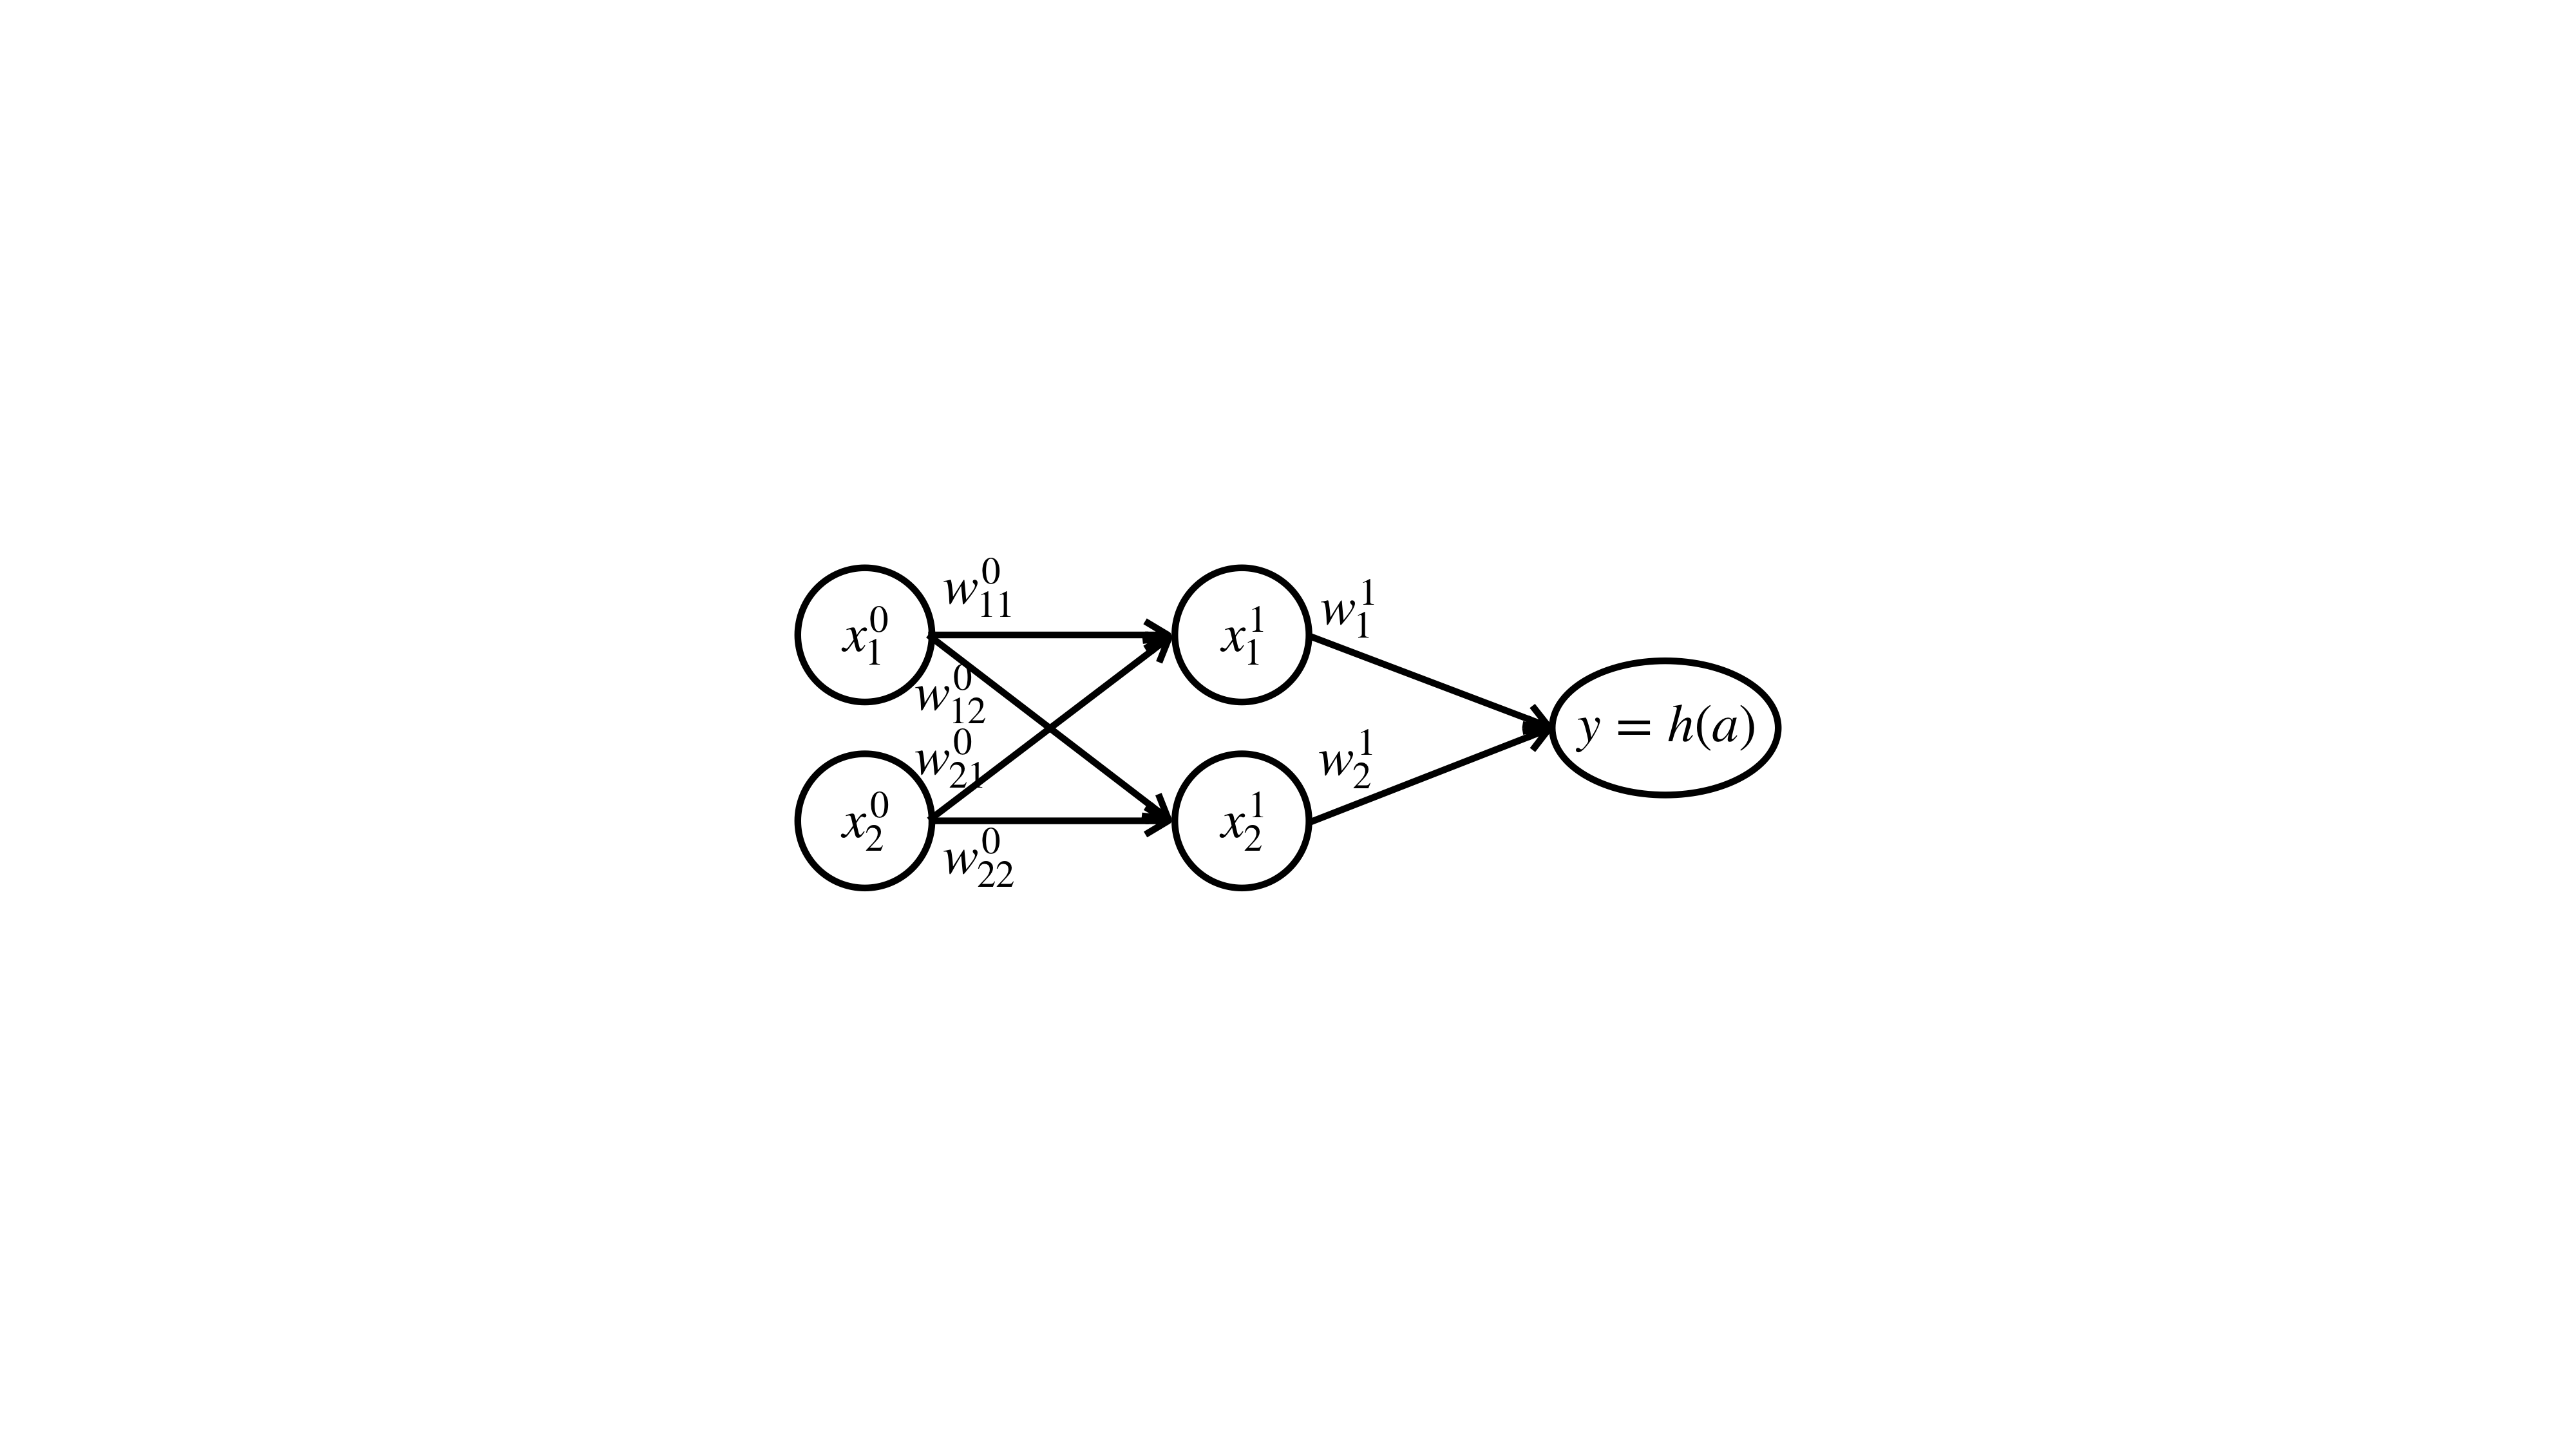
\includegraphics[trim = 250 350 250 350, width=0.9\textwidth, clip]{Figure/2DeepLearning/4MultiLayerPerceptron.png}
 \caption[多層パーセプトロン]{多層パーセプトロン。図\ref{2SimplePerceptron}と同様にノードを繋ぐそれぞれの線は学習可能な重みを表現している。前方のノードは後方のノードの全てと接続されている点にも注意が必要である。}
 \label{4MultiLayerPerceptron}
\end{figure}

多層パーセプトロンは単純パーセプトロンとは異なり, 入力, 出力以外に, 中間層 (隠れ層) を持っている。
ここで, 中間層を$x^1_1,x^1_2$と置くと, 単純パーセプトロンと同様に入力$x^0_1,x^0_2$とそれぞれの重み$w^0_{11},w^0_{12},w^0_{21},w^0_{22}$を用いて
\begin{equation}
 \begin{split}
  x^1_1 = w^0_{11}x^0_1 + w^0_{21}x^0_2 \\
  x^1_2 = w^0_{12}x^0_1 + w^0_{22}x^0_2
 \end{split} 
\end{equation}
と計算でき, また出力$y$についても, $x^1_1,x^1_2$とそれぞれの重み$w^1_{1},w^1_{2}$を用いて, 
\begin{equation}
 \begin{split}
  y &= h(a)\\
  a &= w^1_{1}x^1_1 + w^1_{2}x^1_2
 \end{split}
\end{equation}
となる。

以後, 特に断らない場合はあるノード$x$, 重み$w$について, 層の深さ, 前後のノードを次のように表現する。
\begin{equation}
 \begin{split}
  &x^{({\rm 層の深さ})}_{({\rm ノード番号})}\\
  &w^{({\rm 層の深さ})}_{({\rm 前のノード番号})\ ({\rm 後ろのノード番号})}
 \end{split}
\end{equation}

多層パーセプトロンは, 学習の手法や層を重ねるに連れて重みが更新出来なくなる勾配消失問題など様々な課題を抱えていた。
次節ではこれらの問題を後述する誤差逆伝播法 (Backpropagation) や活性化関数によって解決したニューラルネットワークについて解説する。


%%%%%%%%%%%%%%%%%%%%%%%%%%%%%%%%%%%%%%%%%%%%%%%%%%%%%%%%%%%%%%%%%%%%%%%%%%%%%%%%%%%%%%%%%%%%%%%%%%%%%
\section{ニューラルネットワーク} \label{DL:NeuralNetwork}

本節ではニューラルネットワークについて解説を行う。
ただし, ここでは計算手法や言葉の定義についてのみ述べる。
実装方法については現在様々なフレームワーク\cite{TensorflowWeb, KerasWeb, PyTorchWeb, CaffeWeb}があり, それぞれで実装の仕方が異なっている。
本研究ではtensorflow-kerasを用いた。\footnote{具体的なコードに関しては付録\ref{sec:Code}を参照。}

ニューラルネットワークに関する技術は「ニューラルネットワークの構造」についてと「ニューラルネットワークの学習」についてに大きく分けられると考えている。
前者は主に入力から出力までのネットワークの構築を, 後者は構築されたネットワークの重み更新についての技術である。


%%%%%%%%%%%%%%%%%%%%%%%%%%%%%%%%%%%%%%%%%%%%%%%%%%%%%%%%%%%%%%%%%%%%%%%%
\subsection{ニューラルネットワークの構造} \label{DL:NN:StructureofNN}

ニューラルネットワークは様々な技術によって支えられているが, その基本構造は前節の多層パーセプトロンと全く同じである。
ニューラルネットワークと多層パーセプトロンとの大きな構造の違いは活性化関数である。
ニューラルネットワークでは様々な活性化関数が提案されており\footnote{多層パーセプトロンはニューラルネットワークの内, 活性化関数に階段関数を使った特別なネットワークであると再定義できる。}, これが勾配消失問題を解消する鍵となっている。
活性化関数は重み更新のために微分可能な関数である必要があるが, どのような関数を選ぶかはユーザーに委ねられている。
勾配消失や重み更新についての詳しい解説は\ref{DL:NN:TrainingofNN}節で行う。
以下に活性化関数の例を示す(図\ref{5ActivationFunction})。
\begin{itemize}
  \item 階段関数
\begin{equation}
 h(a) = \left\{ \begin{array}{ll}
    0 & (a \leqq \theta) \\
    1 & (a > \theta)
 \end{array} \right.
\end{equation}
  \item シグモイド関数
\begin{equation}
 h(a) = \frac{1}{1+\exp{(-a)}}
\end{equation}
  \item tanh関数
\begin{equation}
 h(a) = \tanh{(a)}
\end{equation}
  \item ReLU (Rectified Linear Unit, ランプ) 関数\cite{ReLUpaper}
\begin{equation}
 h(a) = \left\{ \begin{array}{ll}
    0 & (a \leqq \theta) \\
    a & (a > \theta)
 \end{array} \right.
\end{equation}
\end{itemize}

\begin{figure}[htbp]
 \centering
 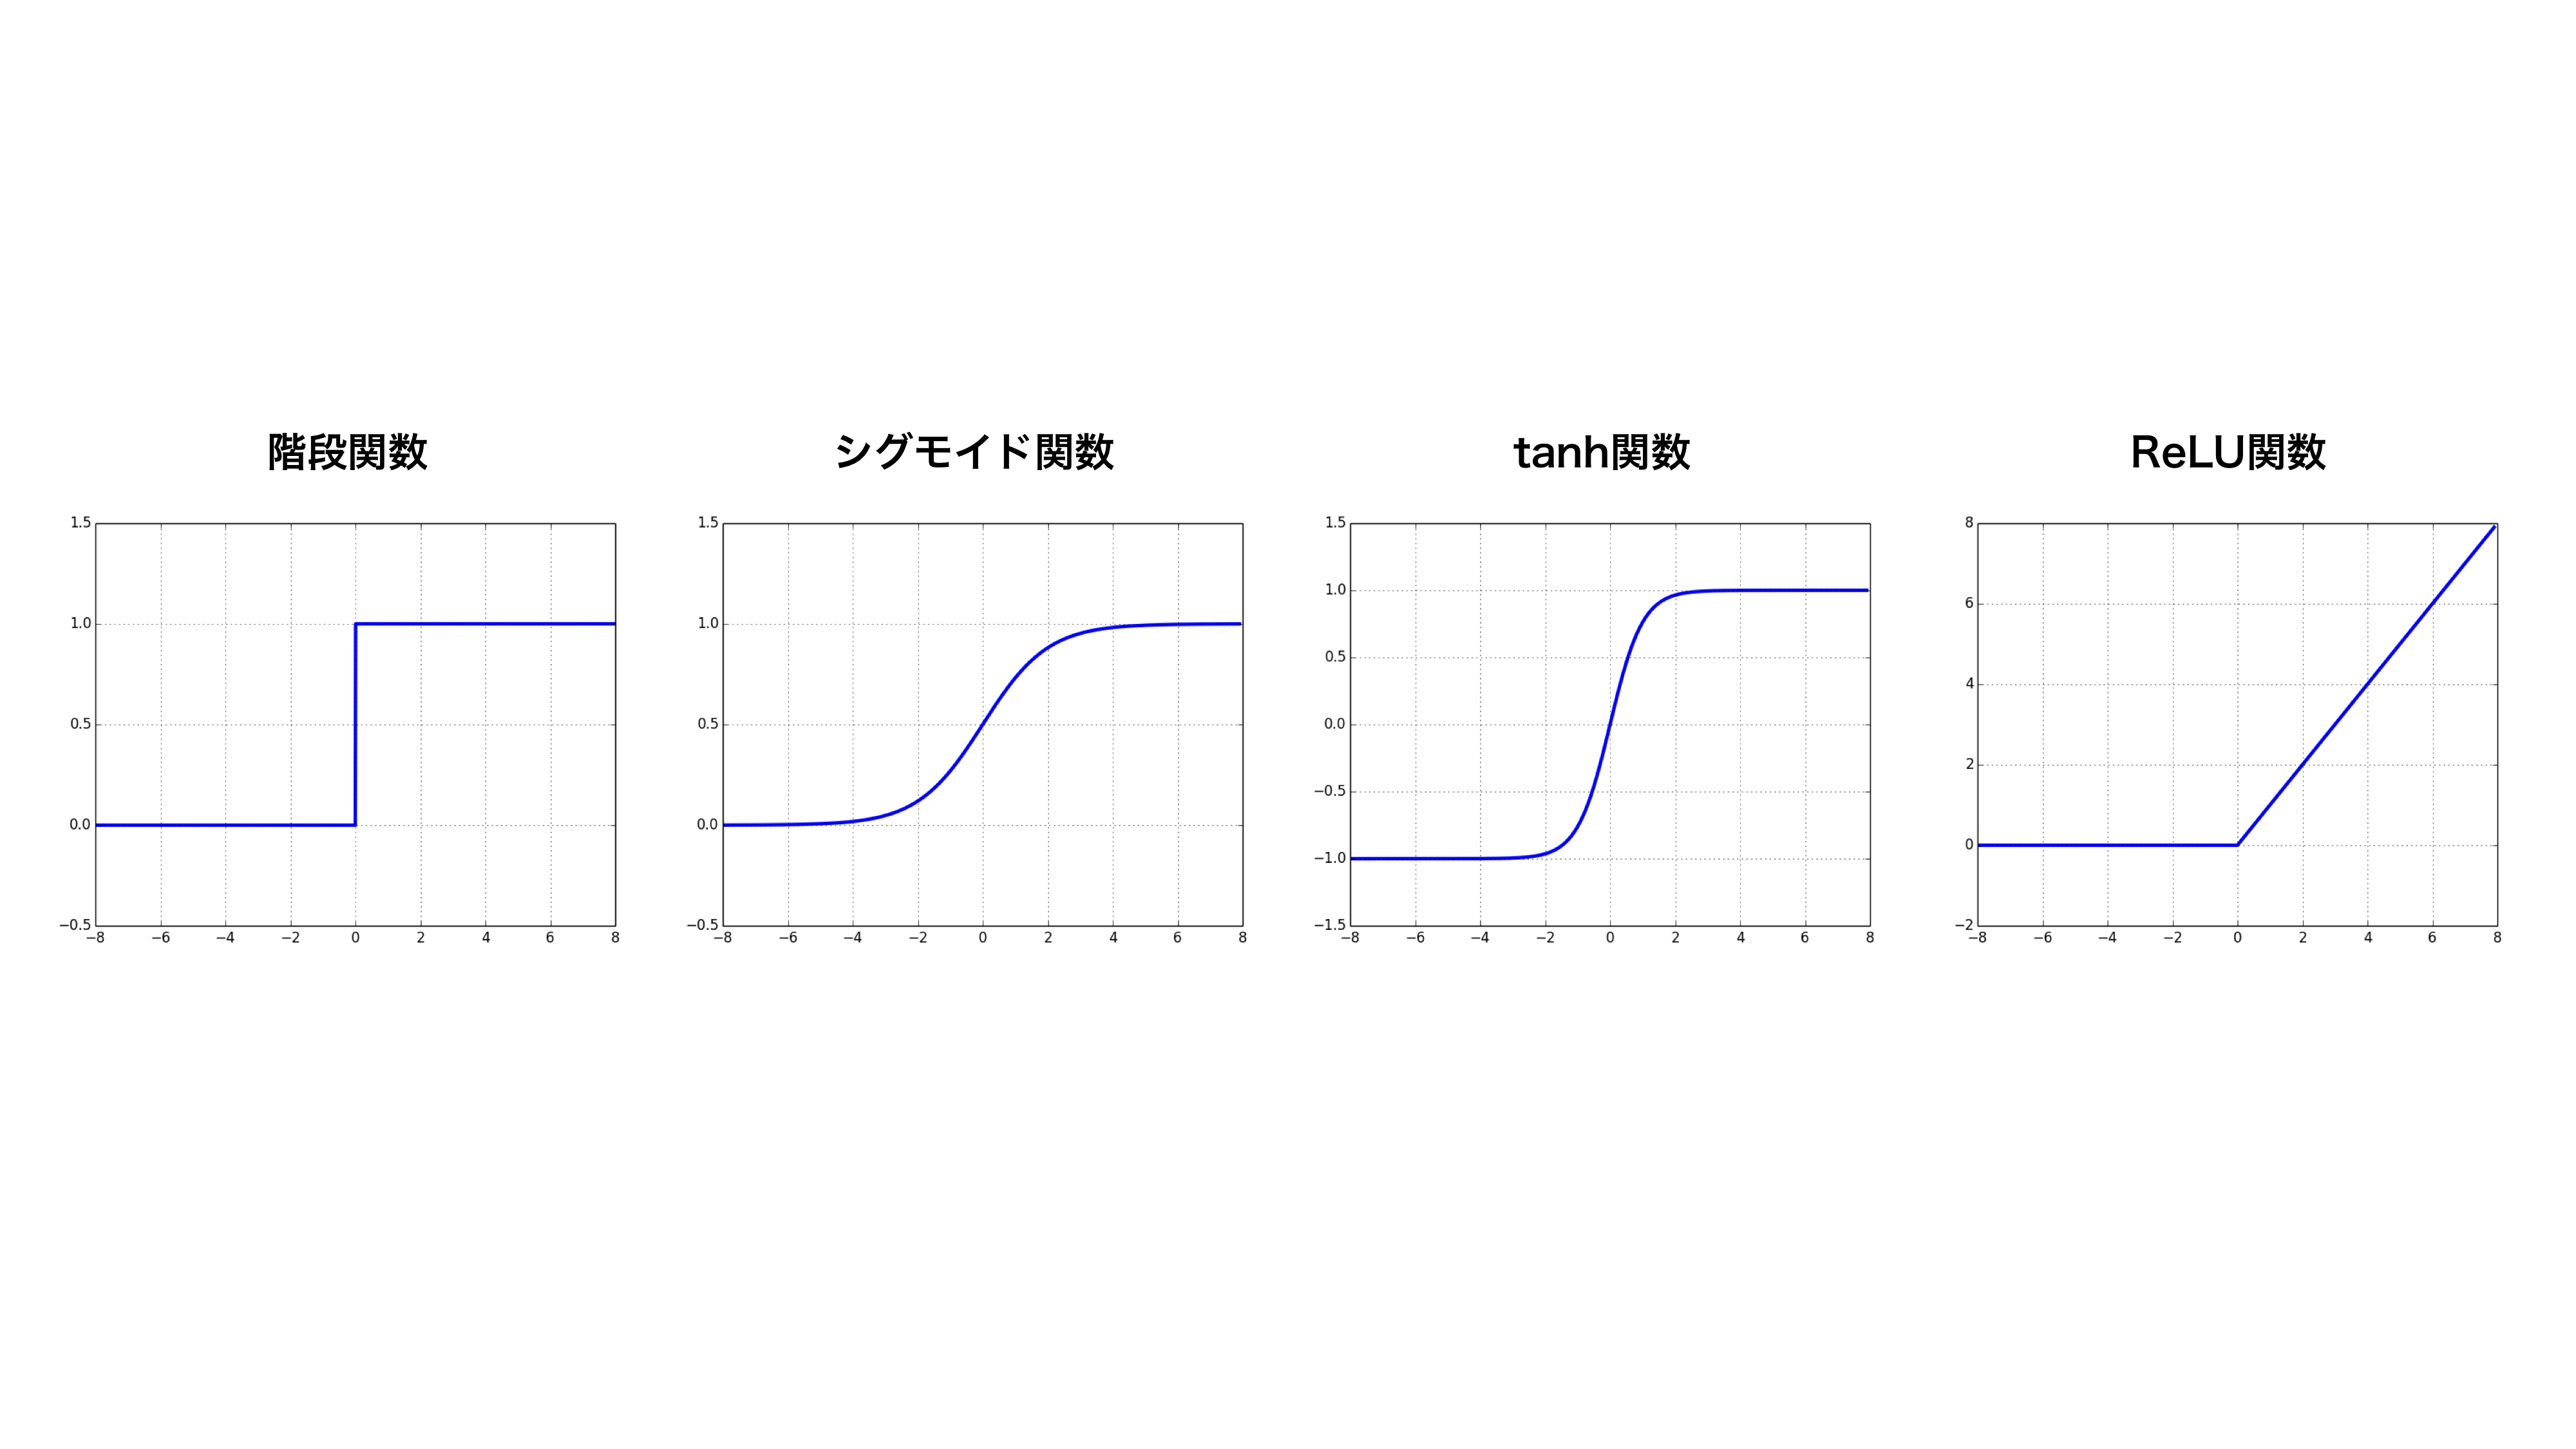
\includegraphics[trim = 0 250 0 250, width=1.0\textwidth, clip]{Figure/2DeepLearning/5ActivationFunction.png}
 \caption{活性化関数}
 \label{5ActivationFunction}
\end{figure}

一般に, ニューラルネットワークは多層パーセプトロンと同様の構造であるので, 図\ref{6NeuralNetwork}のように表現出来る。

\begin{figure}[htbp]
 \centering
 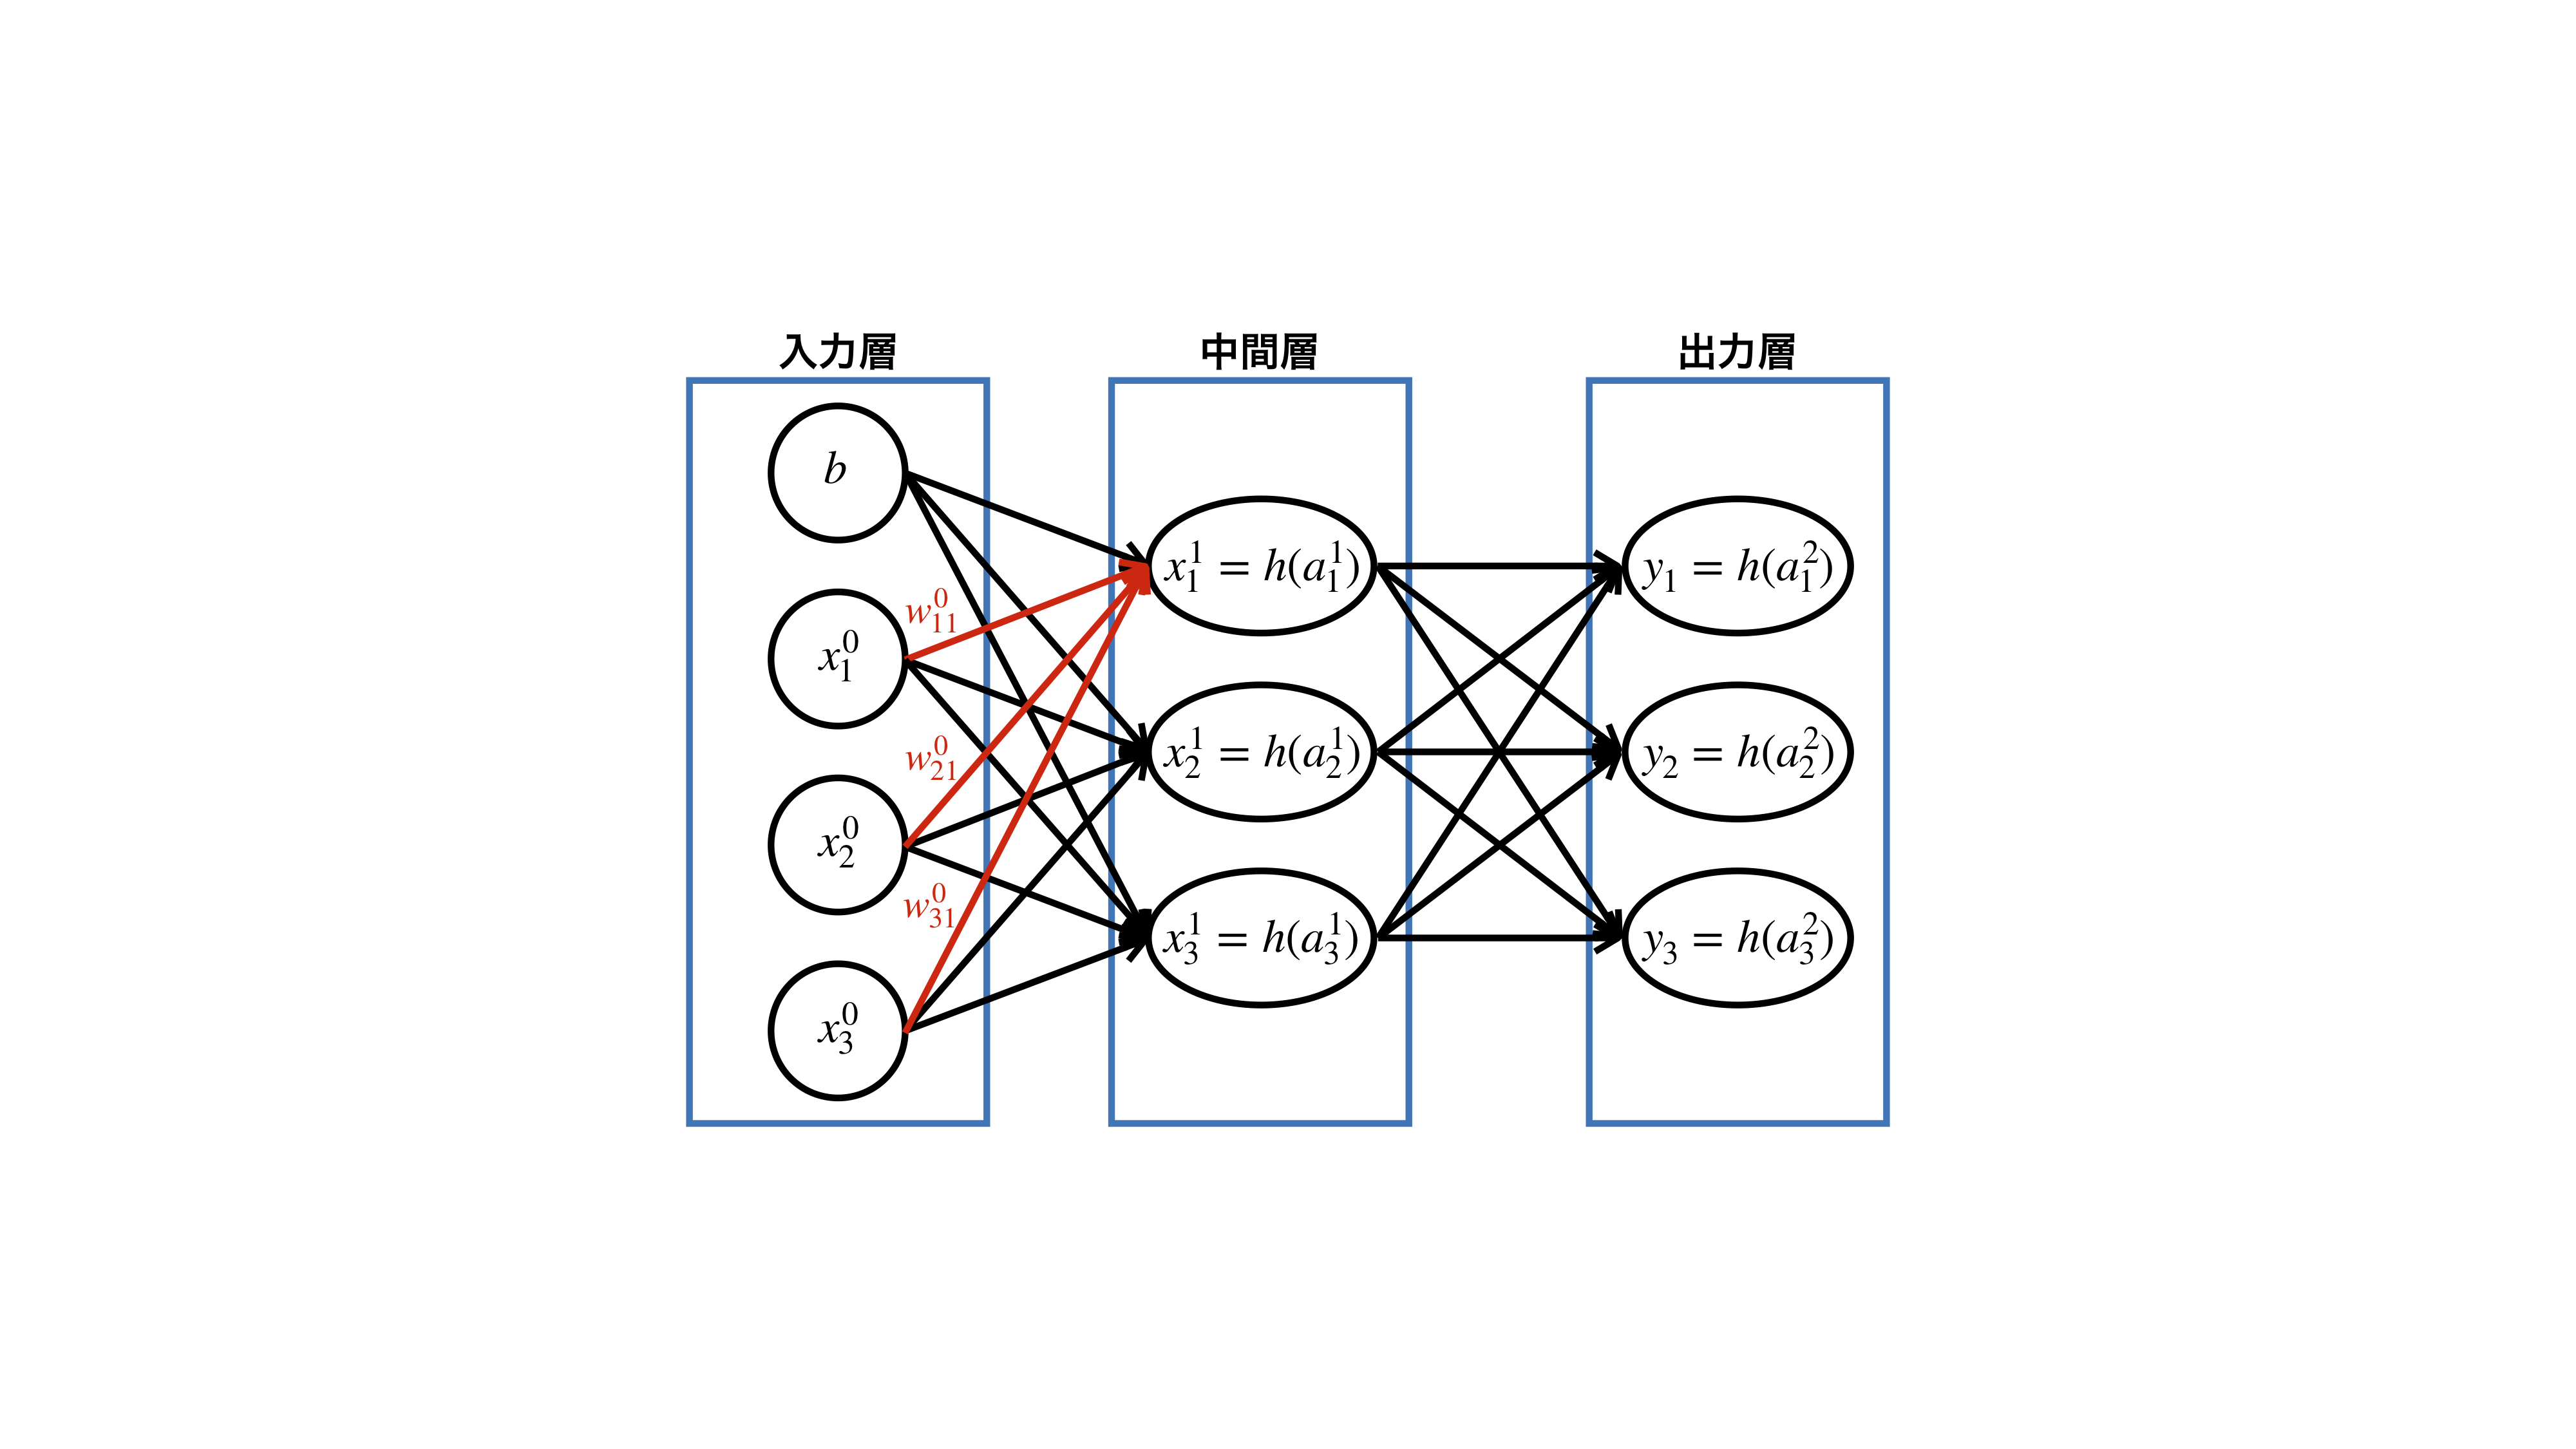
\includegraphics[trim = 250 200 250 200, width=0.9\textwidth, clip]{Figure/2DeepLearning/6NeuralNetwork.png}
 \caption[ニューラルネットワーク]{ニューラルネットワーク。基本構造は多層パーセプトロンと同様であるとわかる。赤線は中間層$x^1_1$へ入力される重みである。}
 \label{6NeuralNetwork}
\end{figure}

ここで, 中間層$x^1_1$は入力$x^0_1,x^0_2,x^0_3$とそれぞれの重み$w^0_{11},w^0_{21},w^0_{31}$を用いて, 
\begin{equation}
 \begin{split}
  x^1_1 &= h(a^1_1)\\
  a^1_1 &= w^0_{11}x^0_1 + w^0_{21}x^0_2 + w^0_{31}x^0_3 + b^0_1
 \end{split}
\end{equation}
と計算できる。
また, バイアスとして$b$を導入している。
これはパーセプトロンの閾値$\theta$に対応している。
中間層$x^1_2,x^1_3$についても同様に, 
\begin{equation}
 \begin{split}
  x^1_2 &= h(a^1_2)\\
  a^1_2 &= w^0_{12}x^0_1 + w^0_{22}x^0_2 + w^0_{32}x^0_3 + b^0_2\\
  x^1_3 &= h(a^1_3)\\
  a^1_3 &= w^0_{13}x^0_1 + w^0_{23}x^0_2 + w^0_{33}x^0_3 + b^0_3
 \end{split}
\end{equation}
と書ける。

また, これら$x^1_1,x^1_2,x^1_3$の計算は行列とベクトルを用いて, より簡潔に表現できる。
\begin{equation}
 \begin{split}
  {\mbox{\boldmath{$x$}}}^1&=
  \left(
    \begin{array}{ccc}
      x^1_1 \\
      x^1_2 \\
      x^1_3 
    \end{array}
  \right)=
  h({\mbox{\boldmath{$a$}}}^1)\\
  {\mbox{\boldmath{$a$}}}^1&=
  \left(
    \begin{array}{ccc}
      a^1_1 \\
      a^1_2 \\
      a^1_3 
    \end{array}
  \right)
  =
  W^0{\mbox{\boldmath{$x$}}}^0 + {\mbox{\boldmath{$b$}}}^0
  =
  \left(
    \begin{array}{ccc}
      w^0_{11} & w^0_{21} & w^0_{31} \\
      w^0_{12} & w^0_{22} & w^0_{32} \\
      w^0_{13} & w^0_{23} & w^0_{33}
    \end{array}
  \right)
  \left(
    \begin{array}{ccc}
      x^0_1 \\
      x^0_2 \\
      x^0_3
    \end{array}
  \right)
  +
  \left(
    \begin{array}{ccc}
      b^0_1 \\
      b^0_2 \\
      b^0_3
    \end{array}
  \right)
 \end{split}
\end{equation}
行列$W^0$とベクトル${\mbox{\boldmath{$b$}}}^0$は学習可能な重みであり, 得られた新たな状態ベクトル${\mbox{\boldmath{$a$}}}^1$は微分可能な任意の活性化関数$h$によって, 中間層${\mbox{\boldmath{$x$}}}^1$へと変換される。
以下, これを繰り返すことによって, ネットワークは構築されている。

出力層における活性化関数は一般に回帰問題では恒等関数を, 分類問題ではソフトマックス関数と呼ばれる関数を使用する。
回帰問題において, 最終的な出力は数値 (連続値) であるため, 恒等関数によって, 変換を行わずそのまま出力することが一般である。

\begin{equation}
 y_k = h(a^2_k) = a^2_k
\end{equation}

一方で, 分類問題では, 最終的な出力は分類されたクラスとなるため, 以下のようなソフトマックス関数を使用する。

\begin{equation}
 y_k = h(a^2_k) = \frac{\exp{(a^2_k)}}{\sum^N_{i=1}\exp{(a^2_i)}}
\end{equation}

このソフトマックス関数は, 分母が総和, 分子がその一要素の形をしており, $y_k$をkについて足し合わせると$1$になることがわかる。
このことから, 出力$y_k$はk番目のクラスについての確率として解釈でき, 分類問題において, どのクラスにどの程度該当するかを表現することに相当している。

前述したように, これは最も基本的なニューラルネットワークであり, このような全結合 (Fully connected, Dense) な層を重ねたネットワークを順伝播型 (フィードフォワード) ニューラルネットワーク (Feedforward Neural Network) という。


%%%%%%%%%%%%%%%%%%%%%%%%%%%%%%%%%%%%%%%%%%%%%%%%%%%%%%%%%%%%%%%%%%%%%%%%
\subsection{ニューラルネットワークの学習} \label{DL:NN:TrainingofNN}


教師あり学習であるニューラルネットワークにおける学習は, 損失関数 (コスト関数, Loss function) を最小化するように, 重みを更新していく事で行われる。
損失関数とは, 訓練データの正解ラベルとネットワークの出力がどの程度離れているかを計算するための関数である。
この損失関数は取り組む問題や訓練データの性質によって適切に選択する必要がある。
ここでは, よく使用される損失関数として以下の二つを挙げる。
\begin{itemize}
  \item 交差エントロピー誤差 (Categorical Cross Entropy)
\begin{equation}
 L = - \sum^N_k t_k \log{(y_k)}
\end{equation}
  \item 平均二乗誤差 (Mean Squared Error)
\begin{equation}
 L = \frac{1}{N} \sum^N_k(t_k - y_k)^2
\end{equation}
\end{itemize}
$t_k, y_k$はそれぞれk番目の正解ラベルとクラスの出力 (確率や値) を示している。
分類問題については交差エントロピー誤差が, 回帰問題については平均二乗誤差が主に使用される。

分類問題において, 正解ラベル$t$は, あるクラスに関して0か1かのベクトル (one-hot vector) で表現されることが一般的である。
例えば, 赤, 青, 緑について分類を行う場合 (3クラス分類という) , 赤を$(1, 0, 0)$, 青を$(0, 1, 0)$, 緑を$(0, 0, 1)$と定義する。
また, ネットワークの出力$y$はどのクラスに属するかの確率となっている。
例えば, 赤, 青, 緑がそれぞれ$80\ \%$, $10\ \%$, $10\ \%$の場合は出力$y$は$(0.8,\ 0.1,\ 0.1)$と書ける。
したがって, 正解ラベルを赤とすると損失関数$L$は
\begin{equation}
 \begin{split}
  L &= - \sum^3_k t_k \log{(y_k)} \\
    &= - t_1 \log{y_1} - t_2 \log{y_2} - t_3 \log{y_3} \\
    &= - 1 \cdot \log{0.8}\\
    &= 0.22314...
 \end{split}
\end{equation}
と計算される。

回帰問題において, 出力$y$, 正解ラベル$t$は共に連続値であるため, 平均二乗誤差のような二つの差を用いる損失関数が一般的である。

前述したように, ネットワークの学習はこの損失関数を最小化するように進む。
今, 損失関数は変数$y_k$の関数で表現出来ており, このような関数の最小値を求めるためには, 単に変数$y_k$を用いて偏微分を行い勾配を求めれば良い。
計算機において, このような勾配を求め, 徐々に関数を最小化していく手法を勾配降下法 (Gradient Descent Method) という。
勾配降下法において, 次のステップの変数$y_k'$は次のように計算される。
\begin{equation}
 \begin{split}
  y_k' = y_k - \eta \frac{\partial L}{\partial y_k}
 \end{split}
\end{equation}
ここで, ステップ幅を決定する定数$\eta$をニューラルネットワークにおいて学習率 (learning rate) という。
学習率は0.001などの定数を問題やネットワークによって適切に選ぶ必要がある。
このようなネットワークについて更新されない初期設定のパラメータをハイパーパラメータという。
ハイパーパラメータについては後の\ref{DL:HyperParameter}節で述べる。

ニューラルネットワークにおいて, 各重みを更新するための勾配は連鎖律 (chain rule) を用いて計算される。
これは更新する重みと最小化される損失関数の間に出力層と活性化関数が存在しているためである。\footnote{損失関数はクラスの出力の関数であり, クラスの出力は活性化関数によって計算され, 活性化関数は出力層の関数である。}
具体的には, ある重み行列$W$に対して, 勾配降下法, 連鎖律を考慮すると, 次のステップの重み行列$W'$は
\begin{equation}
 \begin{split}
  W' &= W - \eta \frac{\partial L}{\partial W}\\
    &=
  \left(
    \begin{array}{ccc}
      w_{11} & w_{21} & w_{31} \\
      w_{12} & w_{22} & w_{32} \\
      w_{13} & w_{23} & w_{33}
    \end{array}
  \right)
  - \eta
  \left(
    \begin{array}{ccc}
      \frac{\partial L}{\partial w_{11}} & \frac{\partial L}{\partial w_{21}} & \frac{\partial L}{\partial w_{31}} \\
      \frac{\partial L}{\partial w_{12}} & \frac{\partial L}{\partial w_{22}} & \frac{\partial L}{\partial w_{32}} \\
      \frac{\partial L}{\partial w_{13}} & \frac{\partial L}{\partial w_{23}} & \frac{\partial L}{\partial w_{33}}
    \end{array}
  \right)\\
    &= W - \eta \frac{\partial L}{\partial y}\frac{\partial y}{\partial a}\frac{\partial a}{\partial W}
 \end{split}
\end{equation}
と計算される。

このような最適化問題に関して, いくつかのアルゴリズムが提案されている。
現在は確率的勾配降下法 (Stochastic Gradient Descent, SGD\cite{SGD}) やそれを基礎としたRMSProp\cite{RMSProp}, Adam\cite{Adam}などの手法がよく使用されている。

学習方法における, ニューラルネットワークと多層パーセプトロンの大きな違いは, 重みの更新を出力層から逆伝播させる誤差逆伝播法 (Backpropergation\cite{Backpropagation}) という手法の有無である。
再度, 図\ref{6NeuralNetwork}を考える。
全ての出力, 中間層を行列計算を用いて記述すると, 
\begin{equation}
 \begin{split}
  {\mbox{\boldmath{$a$}}}^1&=
  \left(
    \begin{array}{ccc}
      a^1_1 \\
      a^1_2 \\
      a^1_3 
    \end{array}
  \right)
  =
  W^0{\mbox{\boldmath{$x$}}}^0 + {\mbox{\boldmath{$b$}}}^0
  =
  \left(
    \begin{array}{ccc}
      w^0_{11} & w^0_{21} & w^0_{31} \\
      w^0_{12} & w^0_{22} & w^0_{32} \\
      w^0_{13} & w^0_{23} & w^0_{33}
    \end{array}
  \right)
  \left(
    \begin{array}{ccc}
      x^0_1 \\
      x^0_2 \\
      x^0_3
    \end{array}
  \right)
  +
  \left(
    \begin{array}{ccc}
      b^0_1 \\
      b^0_2 \\
      b^0_3
    \end{array}
  \right)\\
  {\mbox{\boldmath{$x$}}}^1&=h({\mbox{\boldmath{$a$}}}^1)\\
  {\mbox{\boldmath{$a$}}}^2&=
  \left(
    \begin{array}{ccc}
      a^2_1 \\
      a^2_2 \\
      a^2_3 
    \end{array}
  \right)
  =
  W^1{\mbox{\boldmath{$x$}}}^1
  =
  \left(
    \begin{array}{ccc}
      w^1_{11} & w^1_{21} & w^1_{31} \\
      w^1_{12} & w^1_{22} & w^1_{32} \\
      w^1_{13} & w^1_{23} & w^1_{33}
    \end{array}
  \right)
  \left(
    \begin{array}{ccc}
      x^1_1 \\
      x^1_2 \\
      x^1_3
    \end{array}
  \right)\\
 y_k &= \sigma(a^2_k) = \frac{\exp{(a^2_k)}}{\sum^n_{i=1}\exp{(a^2_i)}}
 \end{split}
\end{equation}
と書ける。
ここで, 出力部分のソフトマックス関数を$\sigma$と書いた。

ある重み$w^1_{11}$について考える。
損失関数$L$の重み$w^1_{11}$による偏微分は, 連鎖律を考慮して, 
\begin{equation}
 \begin{split}
  y_1 &= \sigma(a^2_1)\\
  a^2_1 &= w^1_{11} x^1_1 + w^1_{21} x^1_2 + w^1_{31} x^1_3 = \sum^N_{i=1} w^1_{i1} x^1_i
 \end{split}
\end{equation}
より, 
\begin{equation}
 \begin{split}
  \frac{\partial L}{\partial w^1_{11}} 
  &= \frac{\partial L}{\partial y_1}\frac{\partial y_1}{\partial a^2_1}\frac{\partial a^2_1}{\partial w^1_{11}}\\
  &= \frac{\partial L}{\partial y_1}\frac{\partial \sigma(a^2_1)}{\partial a^2_1}x^1_{11}\\
 \end{split}
\end{equation}
と計算できる。

ここで, 勾配の計算に活性化関数の偏微分が常に積の形で含まれていることがわかる。
この活性化関数の偏微分が$0$になり, そこから抜け出せなくなると, その勾配は常に$0$になり消失してしまう, これが勾配消失である。
勾配消失に陥った場合は, 重みが適切に更新されず, 学習が不十分になってしまう。
このような問題は活性化関数を変更することによって改善され, 現在はReLU関数がよく用いられている。

また, 更に浅い層の重み$w^0_{11}$について考えると, 
\begin{equation}
 \begin{split}
  x^2_1 &= h(a^1_1)\\
  a^1_1 &= w^0_{11} x^0_1 + w^0_{21} x^0_2 + w^0_{31} x^0_3 = \sum^N_{i=1} w^1_{i1} x^0_i
 \end{split}
\end{equation}
より, 
\begin{equation}
 \begin{split}
  \frac{\partial L}{\partial w^0_{11}} 
  &= \sum^N_{k} \frac{\partial L}{\partial y_k}\frac{\partial y_k}{\partial a^2_k}\frac{\partial a^2_k}{\partial x^2_1}\frac{\partial x^2_1}{\partial a^1_1}\frac{\partial a^1_1}{\partial w^0_{11}}\\
  &= \sum^N_{k} \frac{\partial L}{\partial y_k}\frac{\partial y_k}{\partial a^2_k}\frac{\partial a^2_k}{\partial x^2_1}\frac{\partial h(a^1_1)}{\partial a^1_1}x^0_{11}\\
  &= \sum^N_{k} \left(\frac{\partial L}{\partial y_k}\frac{\partial y_k}{\partial a^2_k}w^1_{1k}\right)\frac{\partial h(a^1_1)}{\partial a^1_1}x^0_{11}
 \end{split}
\end{equation}
と計算できる。
この計算は更に層を重ねた場合でも同様の手順で行うことができる。

重みの更新は基本的に全ての訓練データを使用するのではなく, 訓練データをいくつかの塊に分け, その塊について損失関数を計算することで行われる。
このような手法をミニバッチ学習と呼ばれる。
(訓練データ全てを用いたものをバッチ学習という。)
ミニバッチ学習に使用されるデータの数をミニバッチサイズ (あるいは単にバッチサイズ) という。
これも後述するハイパーパラメータの一つである。
ミニバッチ学習はバッチ学習と比較して二つの利点が存在する。

一つは膨大なデータを直接処理しなくても良いという点である。
一般に深層学習で使用されるデータは非常に膨大であり, GPUなどのメモリに乗らない場合があるが, ミニバッチ学習ではこれを回避することができる。

もう一つは学習が停滞しづらいという点である。
訓練データと比較してサイズの小さいミニバッチは上記の勾配が0になりづらく, 局所的な最小点での学習の停滞を回避することができる。

ただしミニバッチ学習のバッチサイズが小さくなった場合には, 損失関数が平均化されず学習が不安定になる (収束しなくなる) という問題が生じる場合がある。\footnote{バッチサイズが$1$ ($1$サンプルのみ) のミニバッチ学習をオンライン学習という。}


%%%%%%%%%%%%%%%%%%%%%%%%%%%%%%%%%%%%%%%%%%%%%%%%%%%%%%%%%%%%%%%%%%%%%%%%
\subsection{ディープニューラルネットワーク} \label{DL:NN:DeepNeuralNetwork}

ディープニューラルネットワーク (Deep Neural Network, DNN) という言葉の定義は非常に曖昧である。\footnote{少なくとも私ははっきりとした定義を存じない。}
\ref{DL:MachineandDeepLearning}節で述べたように, 現在は第三期AIブームであると言われている。
これは上述してきた技術的成熟に加え, 計算機の性能が向上したことにより, より層を重ねた (深い) ニューラルネットワークの学習が可能になった結果であると言える。
$2006$年のHintonらによるauto-encoder\cite{Autoencoder}や$2014$年にIanによって提案された敵対的生成ネットワーク (Generative Adversarial Network, GAN\cite{GenerativeAdversarialNetworks}) など, 様々な発展的な応用がなされ, 現在においても毎年のように新しいネットワークが提案されている。
本節で述べたニューラルネットワークはその基盤技術の一部である。
次節以降では, 系列データを扱うためのニューラルネットワークの応用について紹介する。


%%%%%%%%%%%%%%%%%%%%%%%%%%%%%%%%%%%%%%%%%%%%%%%%%%%%%%%%%%%%%%%%%%%%%%%%%%%%%%%%%%%%%%%%%%%%%%%%%%%%%
\section{リカレントニューラルネットワーク} \label{DL:RecurrentNeuralNetwork}

前節で紹介したようなフィードフォワードニューラルネットワークは系列データを扱う際, 重み行列が固定的な大きさでしか保持出来ないという点と直前の系列に依存した学習が出来ないという点に関して課題を抱えている。
これらの課題を解決するために提案されたのが, リカレントニューラルネットワークというネットワーク構造である。
本節では, このリカレントニューラルネットワークについて解説を行う。
リカレントニューラルネットワークは主に系列データ, 特に時系列データを取り扱うためのネットワークである。
このような時系列に関するニューラルネットワークは自然言語処理などの分野で発展し, 音声認識や機械翻訳といった技術に使用されている。
リカレントニューラルネットワークの構造は, フィードフォワードニューラルネットワークと比較すると複雑であるが, 要素計算は全結合であり, 基本的にはその組み合わせで理解できる。
\ref{DL:RNN:ReccurentNeuralNetwork}項では, そのようなリカレントニューラルネットワークの構造と学習について述べる。
その後, リカレントニューラルネットワークの抱える問題と, ゲート (Gate) と記憶セル (Cell) 呼ばれる技術によってその問題を克服した長・短期記憶 (Long Short-Term Memory, LSTM\cite{LSTMpaper}) というネットワークを\ref{DL:RNN:IssueofRNN}項と\ref{DL:RNN:LongShortTermMemory}項でそれぞれ紹介する。


%%%%%%%%%%%%%%%%%%%%%%%%%%%%%%%%%%%%%%%%%%%%%%%%%%%%%%%%%%%%%%%%%%%%%%%%
\subsection{リカレントニューラルネットワークの構造と学習} \label{DL:RNN:ReccurentNeuralNetwork}

リカレントニューラルネットワークの構造は, これまでのフィードフォワードニューラルネットワークとは大きく異なる。
そのネットワーク構造はいくつかの表現方法が存在しているが, 本論文では時間について展開した図で書くこととする。
図\ref{7RecurrentNeuralNetwork}の左側が時間について展開していない図, 右側が時間について展開した図である。
左側では, 時間についての構造をループで表現し, 任意の時間$t$についての入力$x_t$と出力$h_t$を持つネットワークとして表現している。
右側では, 時間についての構造を展開し, 出力や入力を系列情報ととも表現している。
これまでのフィードフォワードネットワークは情報の伝達を左右に描いていたが, このリカレントニューラルネットワークは上下に描き, 系列の流れを左右で表現されることが多い。
図\ref{7RecurrentNeuralNetwork}の右側では, 出力$h$が二つ存在し, 上に進むものを出力に, 右に進むものが次の系列への入力になっていることがわかる。
このように, 現在の出力を次の系列の入力として使うことで, 直前の系列情報への依存性を導入している。

\begin{figure}[htbp]
 \centering
 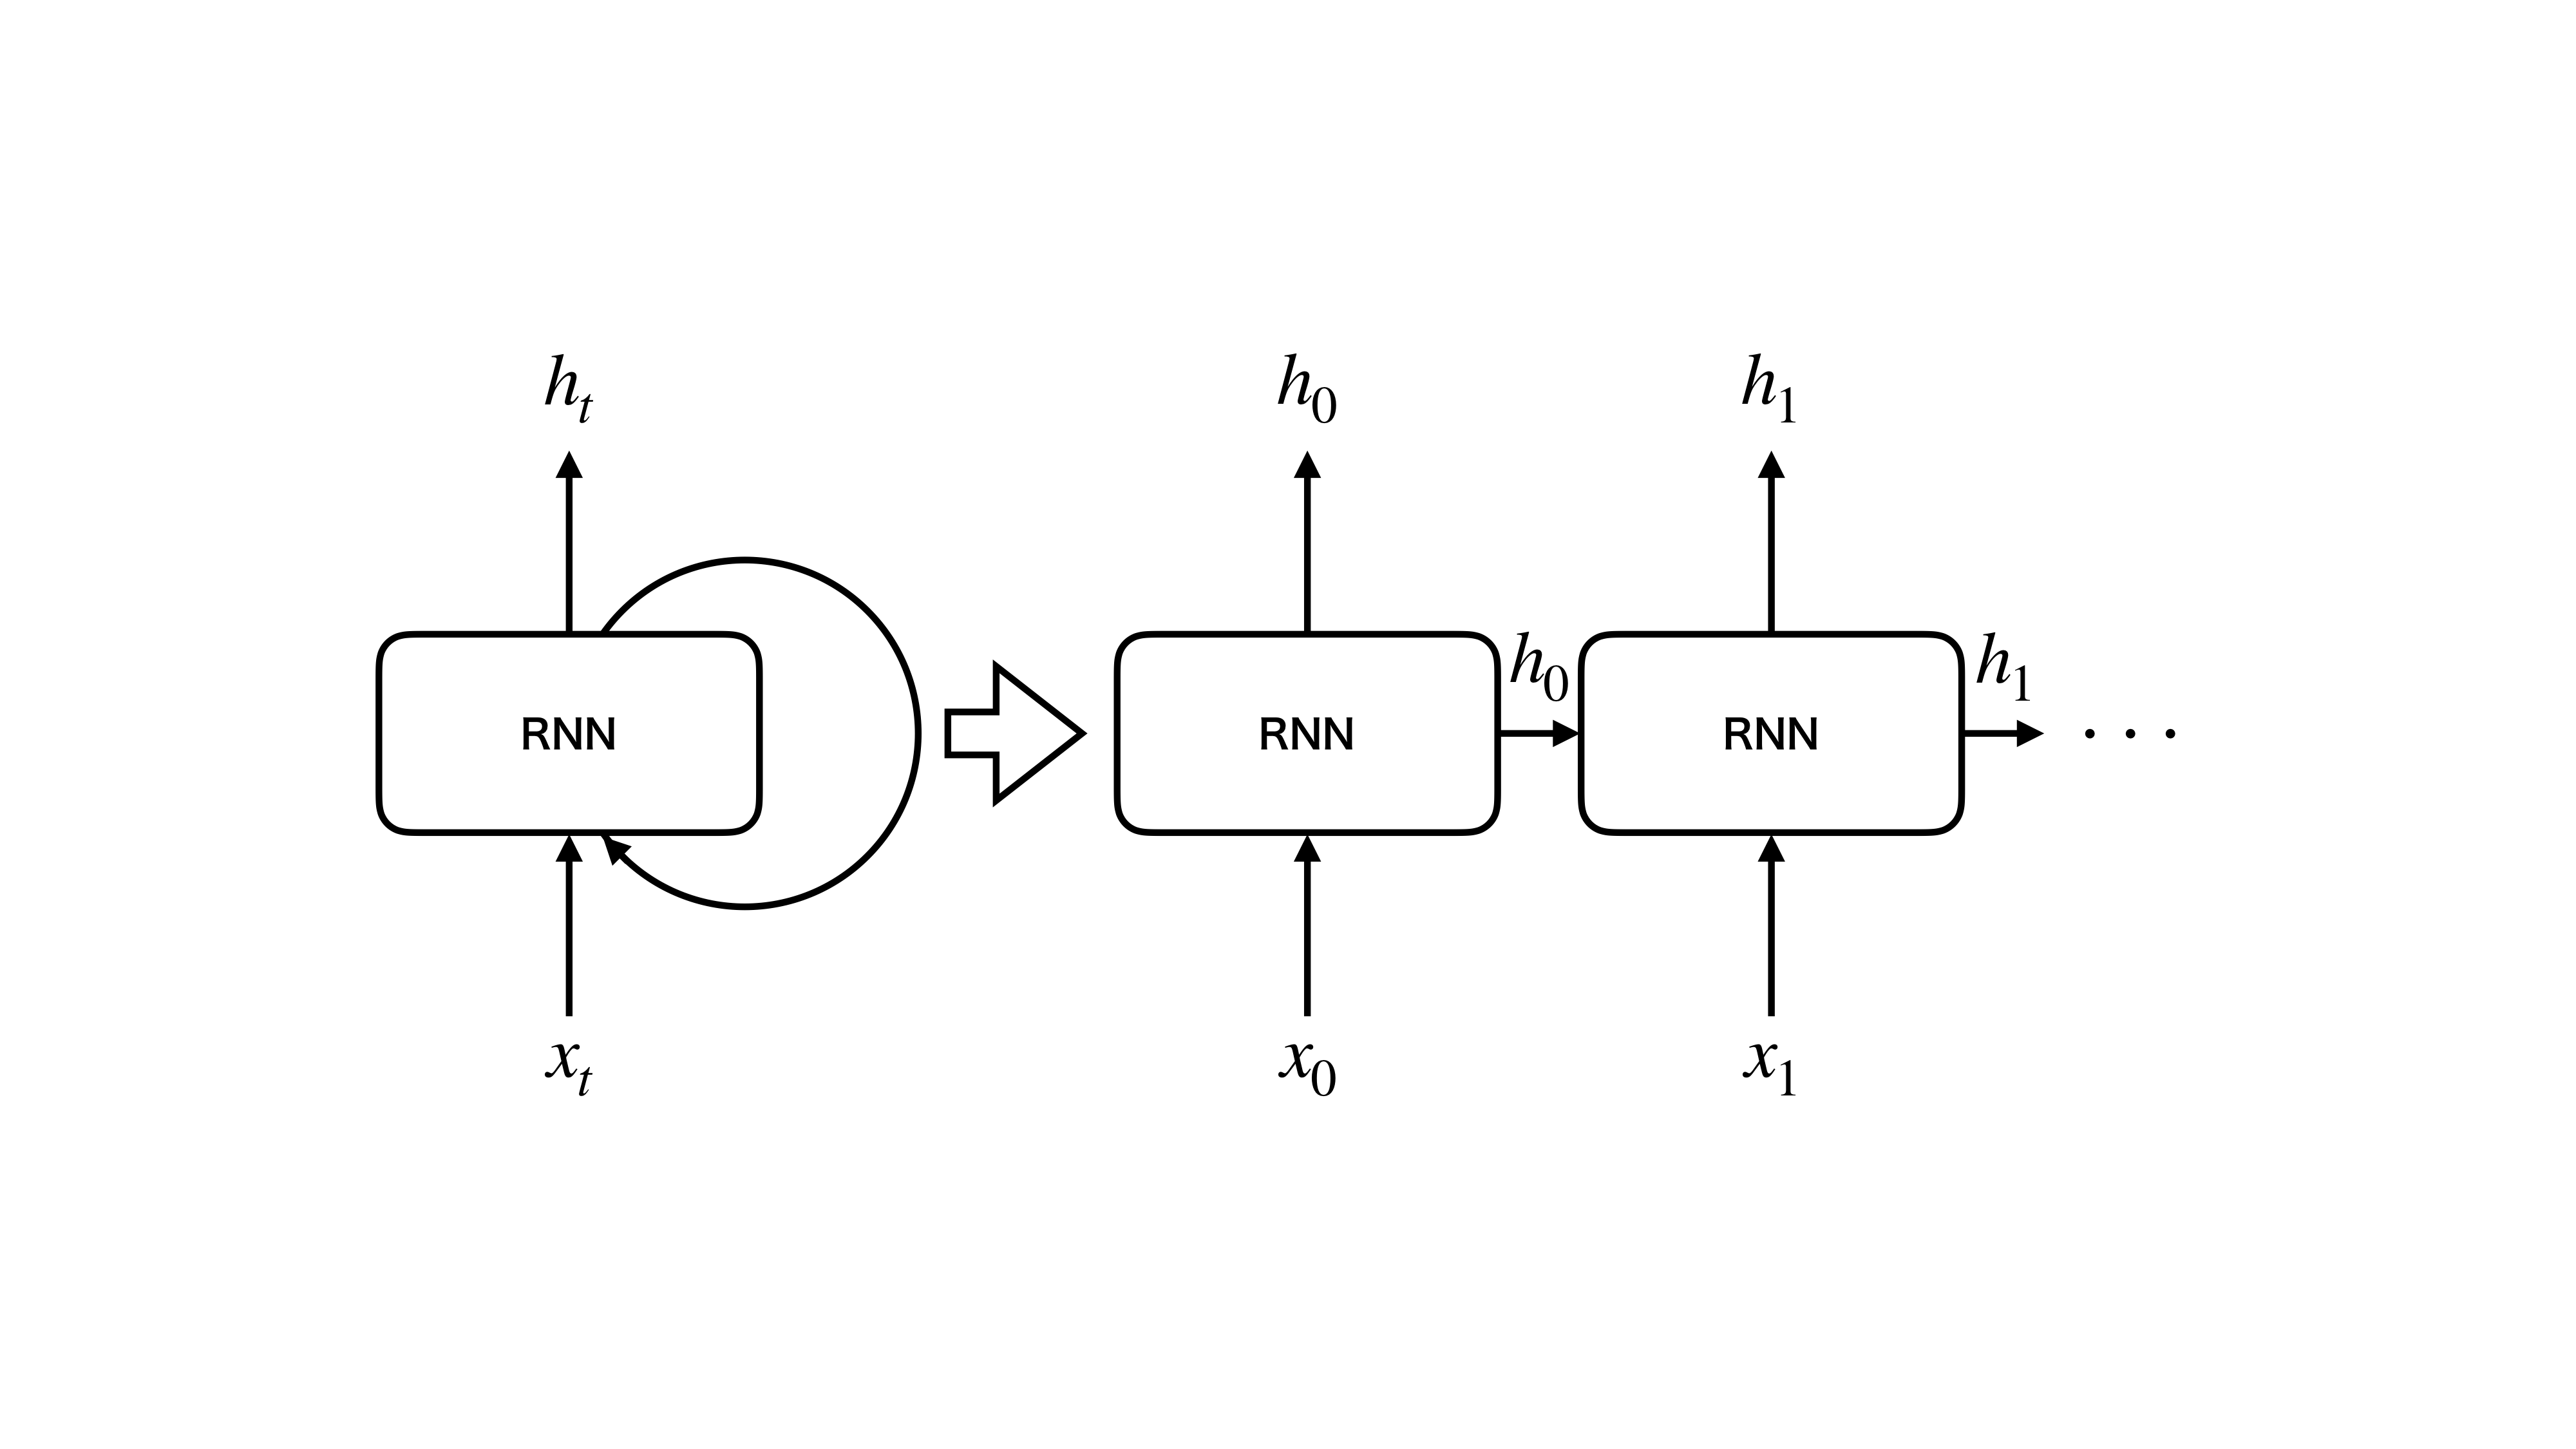
\includegraphics[trim = 0 200 0 200, width=0.9\textwidth, clip]{Figure/2DeepLearning/7RecurrentNeuralNetwork.png}
 \caption[リカレントニューラルネットワーク]{リカレントニューラルネットワーク。図左は時間について展開していない描画方法, 図右は時間について展開した描画方法である。下方から入力され, 上方に出力している。横方向は系列を表現しており, 入力$x_t$は全ての系列で同じ形状でなければならない。}
 \label{7RecurrentNeuralNetwork}
\end{figure}

これまでと同様に明示的にネットワークの重みを描画すると, 図\ref{8RNNWeight}のようになる。
図\ref{7RecurrentNeuralNetwork}のRNNに当たる部分が展開され, 重みを線で表現した図になっている。
図より, 一つ前に系列の出力${\mbox{\boldmath{$h$}}}_{t-1}$と現在の系列の入力${\mbox{\boldmath{$x$}}}_t$を用いて, 現在の系列の出力${\mbox{\boldmath{$h$}}}_t$が生成されていることがわかる。
${\mbox{\boldmath{$h$}}}$についての赤い線に関する重み行列を$W_h$, ${\mbox{\boldmath{$x$}}}$についての黒い線に関する重み行列を$W_x$と置くと, 出力${\mbox{\boldmath{$h$}}}_t$は次のように計算できる。

\begin{figure}[htbp]
 \centering
 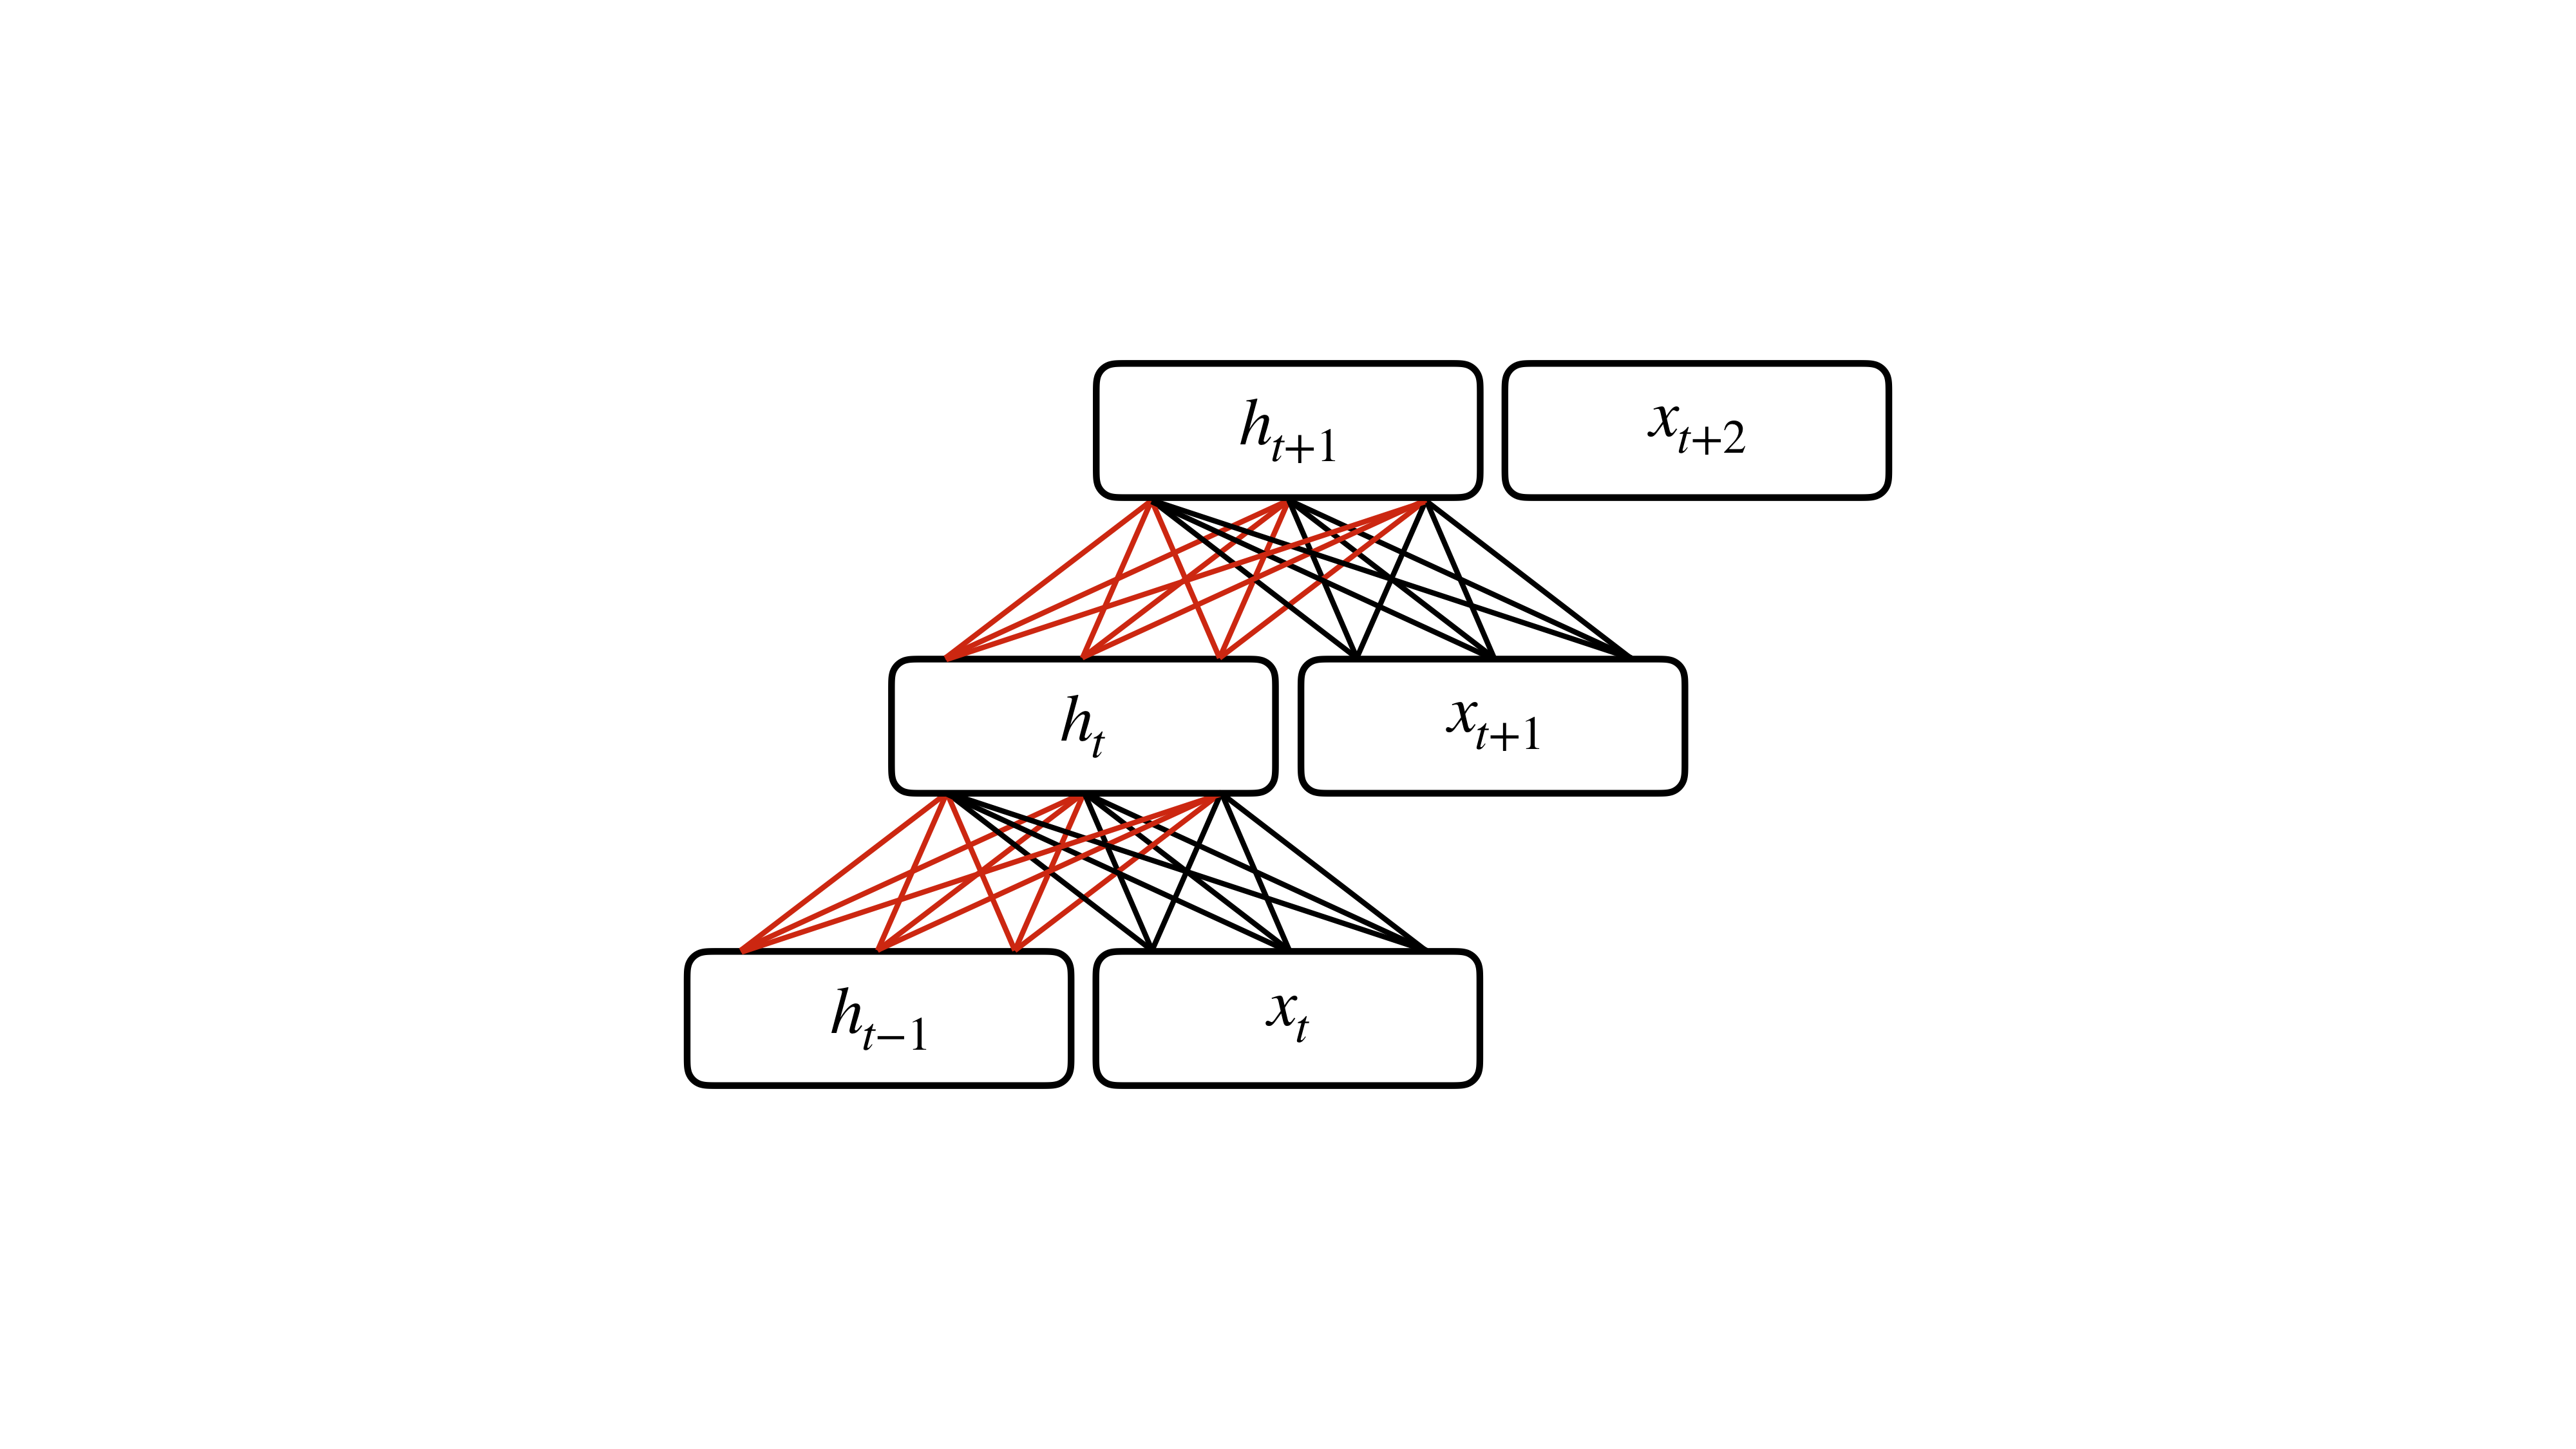
\includegraphics[trim = 0 200 0 200, width=0.9\textwidth, clip]{Figure/2DeepLearning/8RNNWeight.png}
 \caption[リカレントニューラルネットワークの重みの明示的な表現]{リカレントニューラルネットワークの重みの明示的な表現。赤線で示した重みは隠れ状態${\mbox{\boldmath{$h$}}}$についての重み$W_h$, 黒線で示した重みは隠れ層${\mbox{\boldmath{$x$}}}$についての重み$W_x$である。図\ref{7RecurrentNeuralNetwork}で示した"RNN"部はここでは線に相当している。ネットワークは上に積み重なっているように表現しているが, 実際にはこれらの重み行列は全ての系列で同一のものである。}
 \label{8RNNWeight}
\end{figure}

\begin{equation}
 \begin{split}
  {\mbox{\boldmath{$h$}}}_t 
  &= \tanh{(W_h{\mbox{\boldmath{$h$}}}_{t-1}+W_x{\mbox{\boldmath{$x$}}}_t)}\\
  {\mbox{\boldmath{$a$}}}_t 
  &=
  \left(
    \begin{array}{ccc}
      w_{h,11} & w_{h,21} & w_{h,31} \\
      w_{h,12} & w_{h,22} & w_{h,32} \\
      w_{h,13} & w_{h,23} & w_{h,33}
    \end{array}
  \right)
  \left(
    \begin{array}{ccc}
      h_{t-1,1} \\
      h_{t-1,2} \\
      h_{t-1,3}
    \end{array}
  \right)
  +
  \left(
    \begin{array}{ccc}
      w_{x,11} & w_{x,21} & w_{x,31} \\
      w_{x,12} & w_{x,22} & w_{x,32} \\
      w_{x,13} & w_{x,23} & w_{x,33}
    \end{array}
  \right)
  \left(
    \begin{array}{ccc}
      x_{t,1} \\
      x_{t,2} \\
      x_{t,3}
    \end{array}
  \right)
 \end{split}
\end{equation}
リカレントニューラルネットワークでは活性化関数としてtanh関数を使用している。
前述したように, 個々の要素計算はフィードフォワードニューラルネットワークの様に全結合で構成されていることがわかる。
ここで, 非常に重要な性質として, 学習可能な重み行列$W_{h}, W_{x}$は全ての系列$t$について同一のものであり, 大きさが不変であることに注意する。

このように再帰的に重み行列を使用することで, 行列の大きさが可変でないという性質を回避し, 系列情報を取り入れることに成功している。
また, このような入力の系列長についての柔軟性は, 長さが不定であるリアルタイムな時系列データを扱えるという点で重要である。

リカレントニューラルネットワークの出力方法は, 問題によっていくつかのパターンが存在する。(図\ref{9RNNOutputs})
例えば, 語句の分類の様な問題の場合は, 一つの入力に対して, 一つの出力を得るMany to Manyという出力の作り方を行う。
また, 機械翻訳のデコーダーなど, 一つの入力に対して, 複数の出力を得たい場合はOne to Manyを用いる。
最後に, 感情分析の様に複数の入力に対して, 一つの出力を得たい場合はMany to Oneを用いる。

\begin{figure}[htbp]
 \centering
 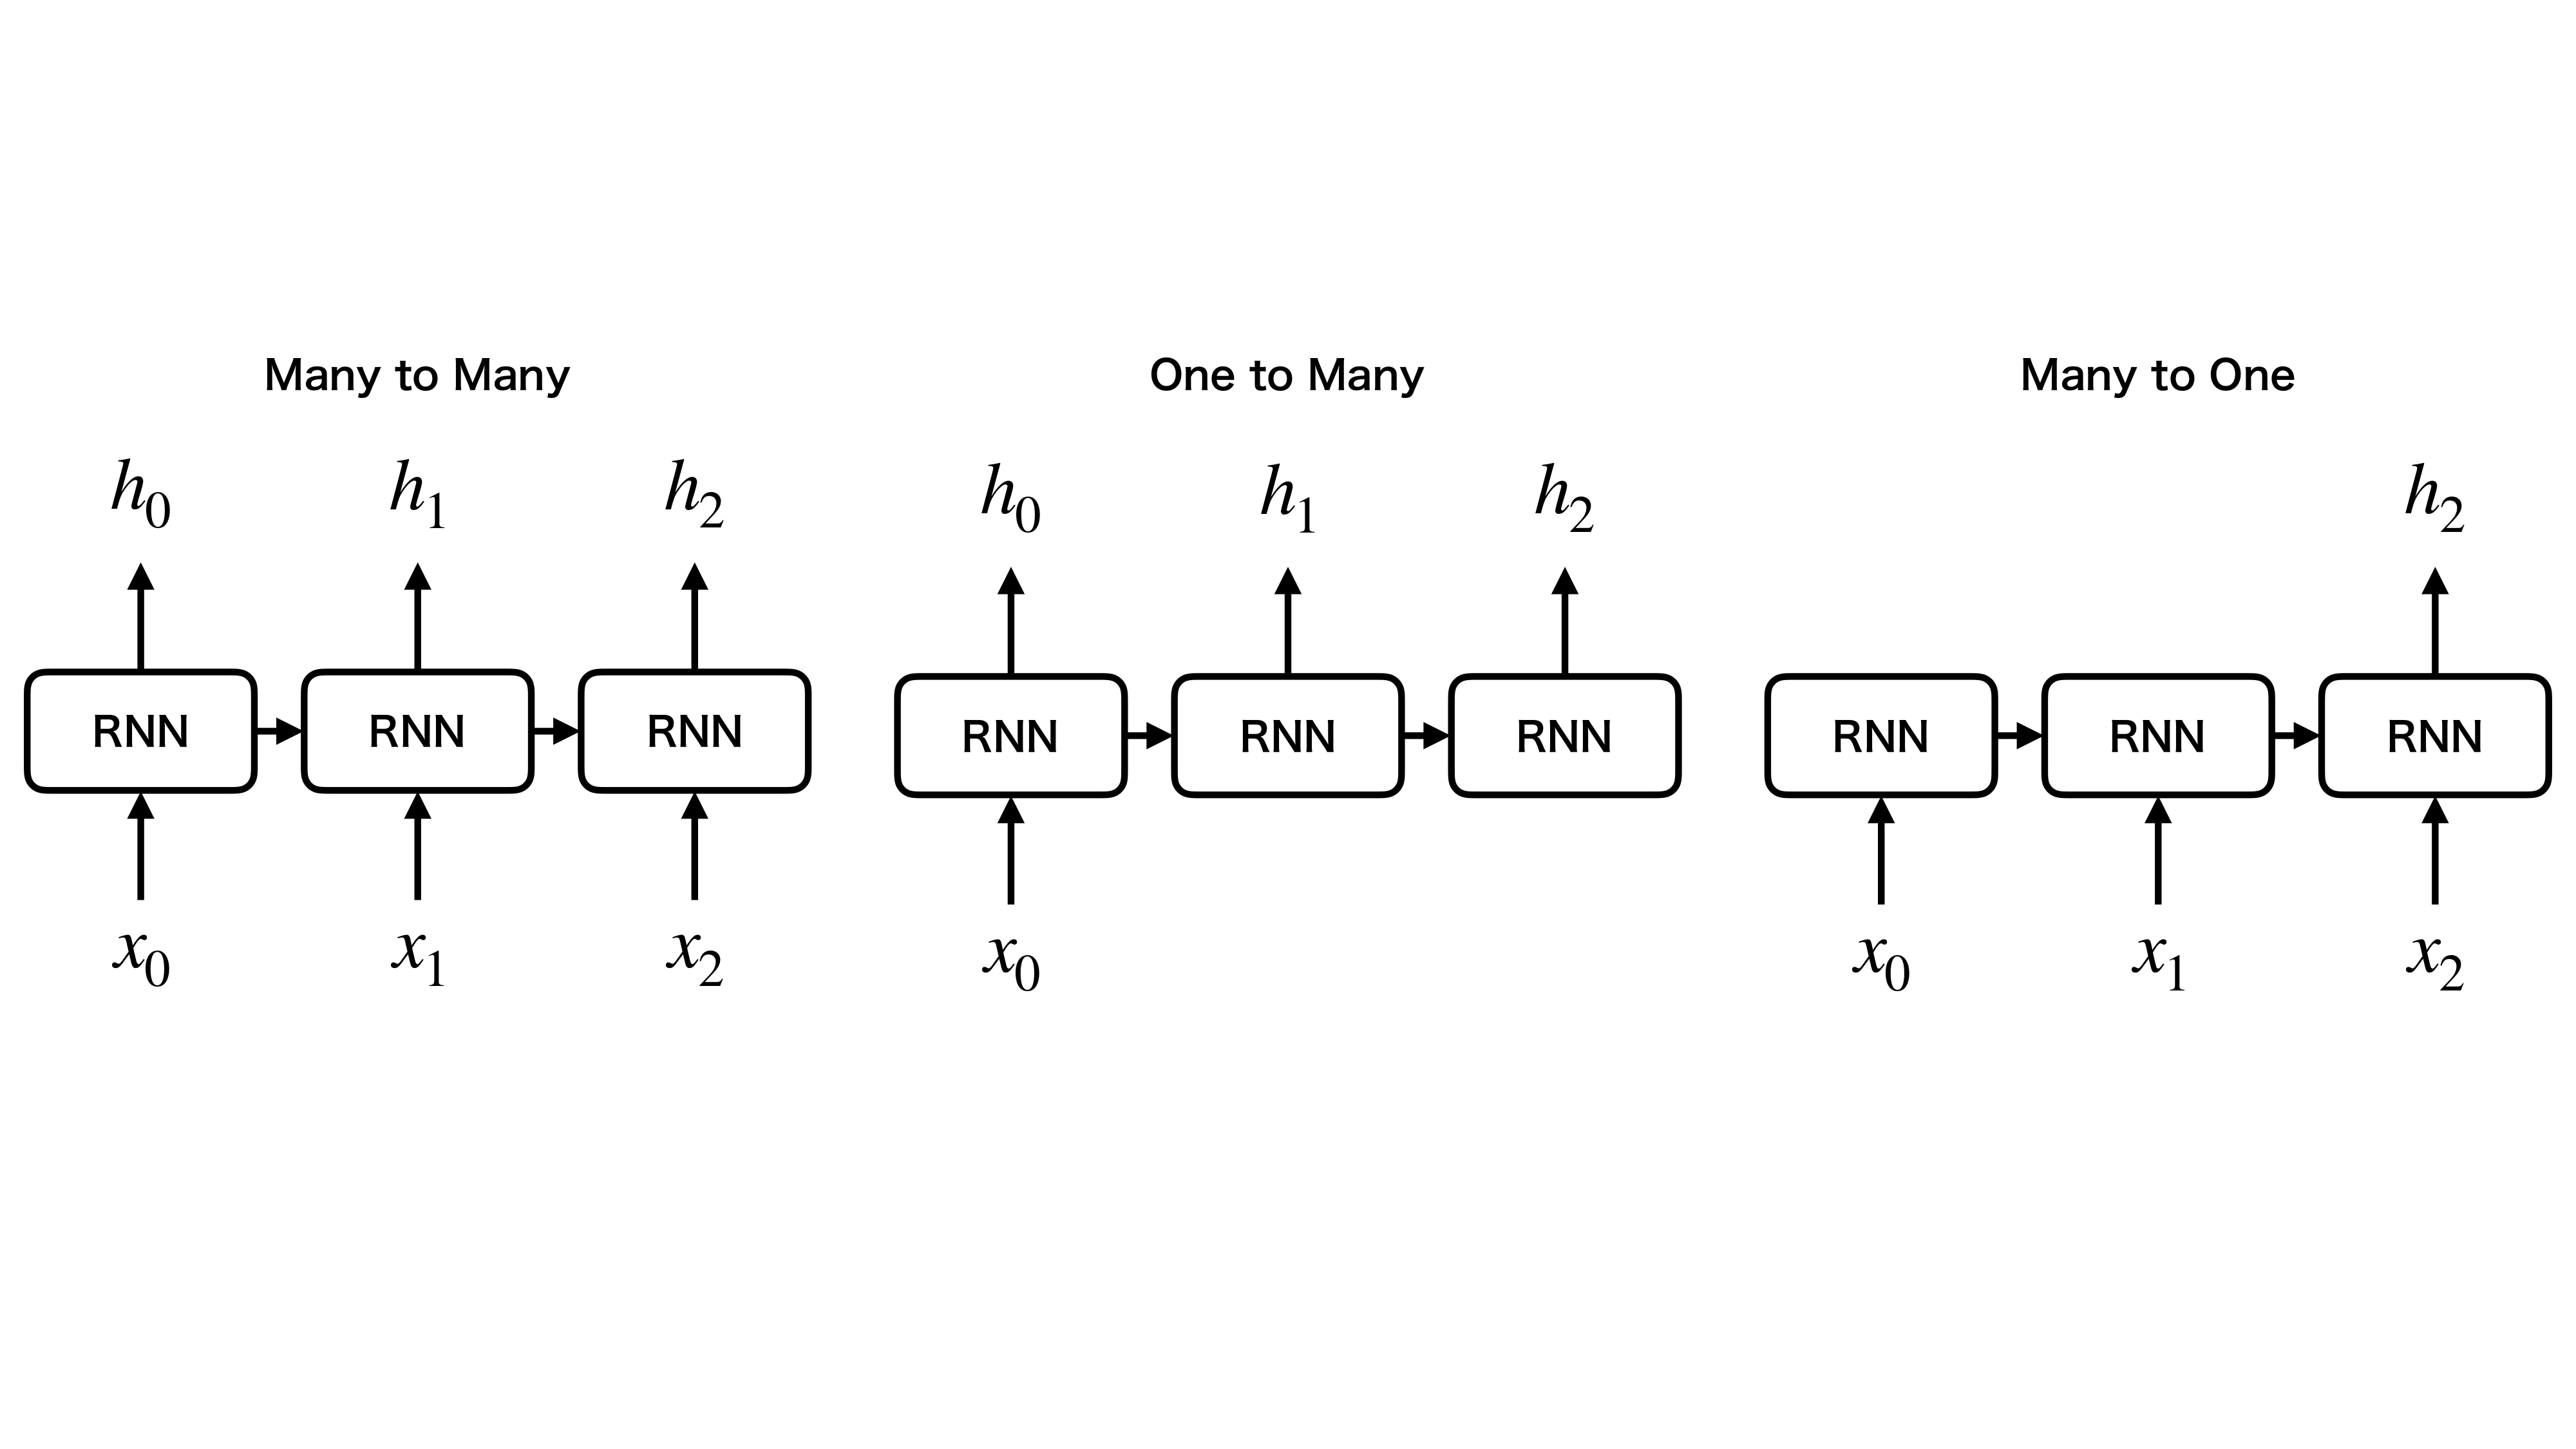
\includegraphics[trim = 0 200 0 200, width=1.0\textwidth, clip]{Figure/2DeepLearning/9RNNOutputs.png}
 \caption[リカレントニューラルネットワークの出力方法]{リカレントニューラルネットワークの出力方法}
 \label{9RNNOutputs}
\end{figure}

リカレントニューラルネットワークの学習は基本的にフィードフォワードニューラルネットワークと同様であるが, 図\ref{8RNNWeight}に見る様にネットワークは系列にしたがって深くなっている。
この為, 重み更新はこの系列を遡って行う必要がある。
このような誤差逆伝播法の事をBackpropagation Through Time (BPTT) という。
実際には計算リソースの削減のため, Truncated BPTTという, 時系列方向に適当な長さで切り取り計算を行う手法が使用される。


%%%%%%%%%%%%%%%%%%%%%%%%%%%%%%%%%%%%%%%%%%%%%%%%%%%%%%%%%%%%%%%%%%%%%%%%
\subsection{リカレントニューラルネットワークの問題点} \label{DL:RNN:IssueofRNN}

リカレントニューラルネットワークは時間方向に展開し, それを遡ることによって学習を行っているため, 系列の長さに依存して非常に深いネットワークが構築される。
したがって, リカレントニューラルネットワークは真に深いネットワークであると言えるが, 深い層からの勾配は非常に消失あるいは爆発しやすく, 容易に勾配消失・爆発を招いてしまうという問題が生じている。
勾配消失はリカレントニューラルネットワークの活性化関数であるtanh関数に起因している。
\ref{DL:NN:TrainingofNN}項で解説したように, 誤差逆伝播法は連鎖律によって計算され, その計算には活性化関数の微分が含まれている。
ここでtanh関数の微分は, 
\begin{equation}
 \begin{split}
  \frac{\partial y(x)}{\partial x}
  &= \frac{\partial}{\partial x} \tanh(x) = \frac{1}{\cosh^2 (x)} \\
  &= 1 - \frac{\cosh^2 (x) - 1}{\cosh^2 (x)} = 1 - \frac{\sinh^2 (x)}{\cosh^2 (x)} = 1 - \tanh^2 (x) = 1 - y^2
 \end{split}
\end{equation}
と計算される。

$1-y^2$は, $y=0$以外において常に1より小さい値を取ってしまう。
リカレントニューラルネットワークでは系列長に応じて, この1より小さい値 ($1-y^2$) が複数回掛けられてしまうため, 勾配消失が生じやすくなっている。
同時にリカレントニューラルネットワークでは, 連鎖律によって系列長に応じて同じ重み行列$W_h$を複数回掛けており, この重み行列の値に応じて, 勾配が発散あるいは消失してしまうことが考えられる。

また, リカレントニューラルネットワークは時系列上の複数の入出力から, 矛盾した重み更新を受け取ってしまう入力重み衝突, 出力重み衝突という問題も抱えている。

更に, リカレントニューラルネットワークはその構造上, 長期的な系列情報を保持できないという課題も存在している。

以上のような問題を解決するため, ゲートとセルと呼ばれる技術を導入したものを, ゲート付きリカレントユニット (Gated Recurrent Unit, GRU\cite{GRU}) という。
次項では, このゲートを用いたリカレントニューラルネットワークの一つであるLSTMについて紹介する。


%%%%%%%%%%%%%%%%%%%%%%%%%%%%%%%%%%%%%%%%%%%%%%%%%%%%%%%%%%%%%%%%%%%%%%%%
\subsection{長・短期記憶 (Long Short-Term Memory, LSTM)} \label{DL:RNN:LongShortTermMemory}

LSTMのネットワーク構造全体を図\ref{10LongShortTermMemory}に示す。
リカレントニューラルネットワークとの最も大きな違いは, LSTMは隠れ状態 (出力) を二つ${\mbox{\boldmath{$h$}}}_t,{\mbox{\boldmath{$c$}}}_t$持っているという点である。
${\mbox{\boldmath{$c$}}}_t$は長期的な記憶セルを示しており, 図\ref{10LongShortTermMemory}では上部の赤い線で表現されている。
一方, ${\mbox{\boldmath{$h$}}}_t$は, リカレントニューラルネットワークと同様に短期的な系列情報の伝達と出力に使用されている。
LSTMは三つの入力${\mbox{\boldmath{$h$}}}_{t-1},{\mbox{\boldmath{$c$}}}_{t-1},{\mbox{\boldmath{$x$}}}_t$を受け取り, 二つの出力${\mbox{\boldmath{$h$}}}_t,{\mbox{\boldmath{$c$}}}_t$を提供するネットワークであるとみなすことができる。

\begin{figure}[htbp]
 \centering
 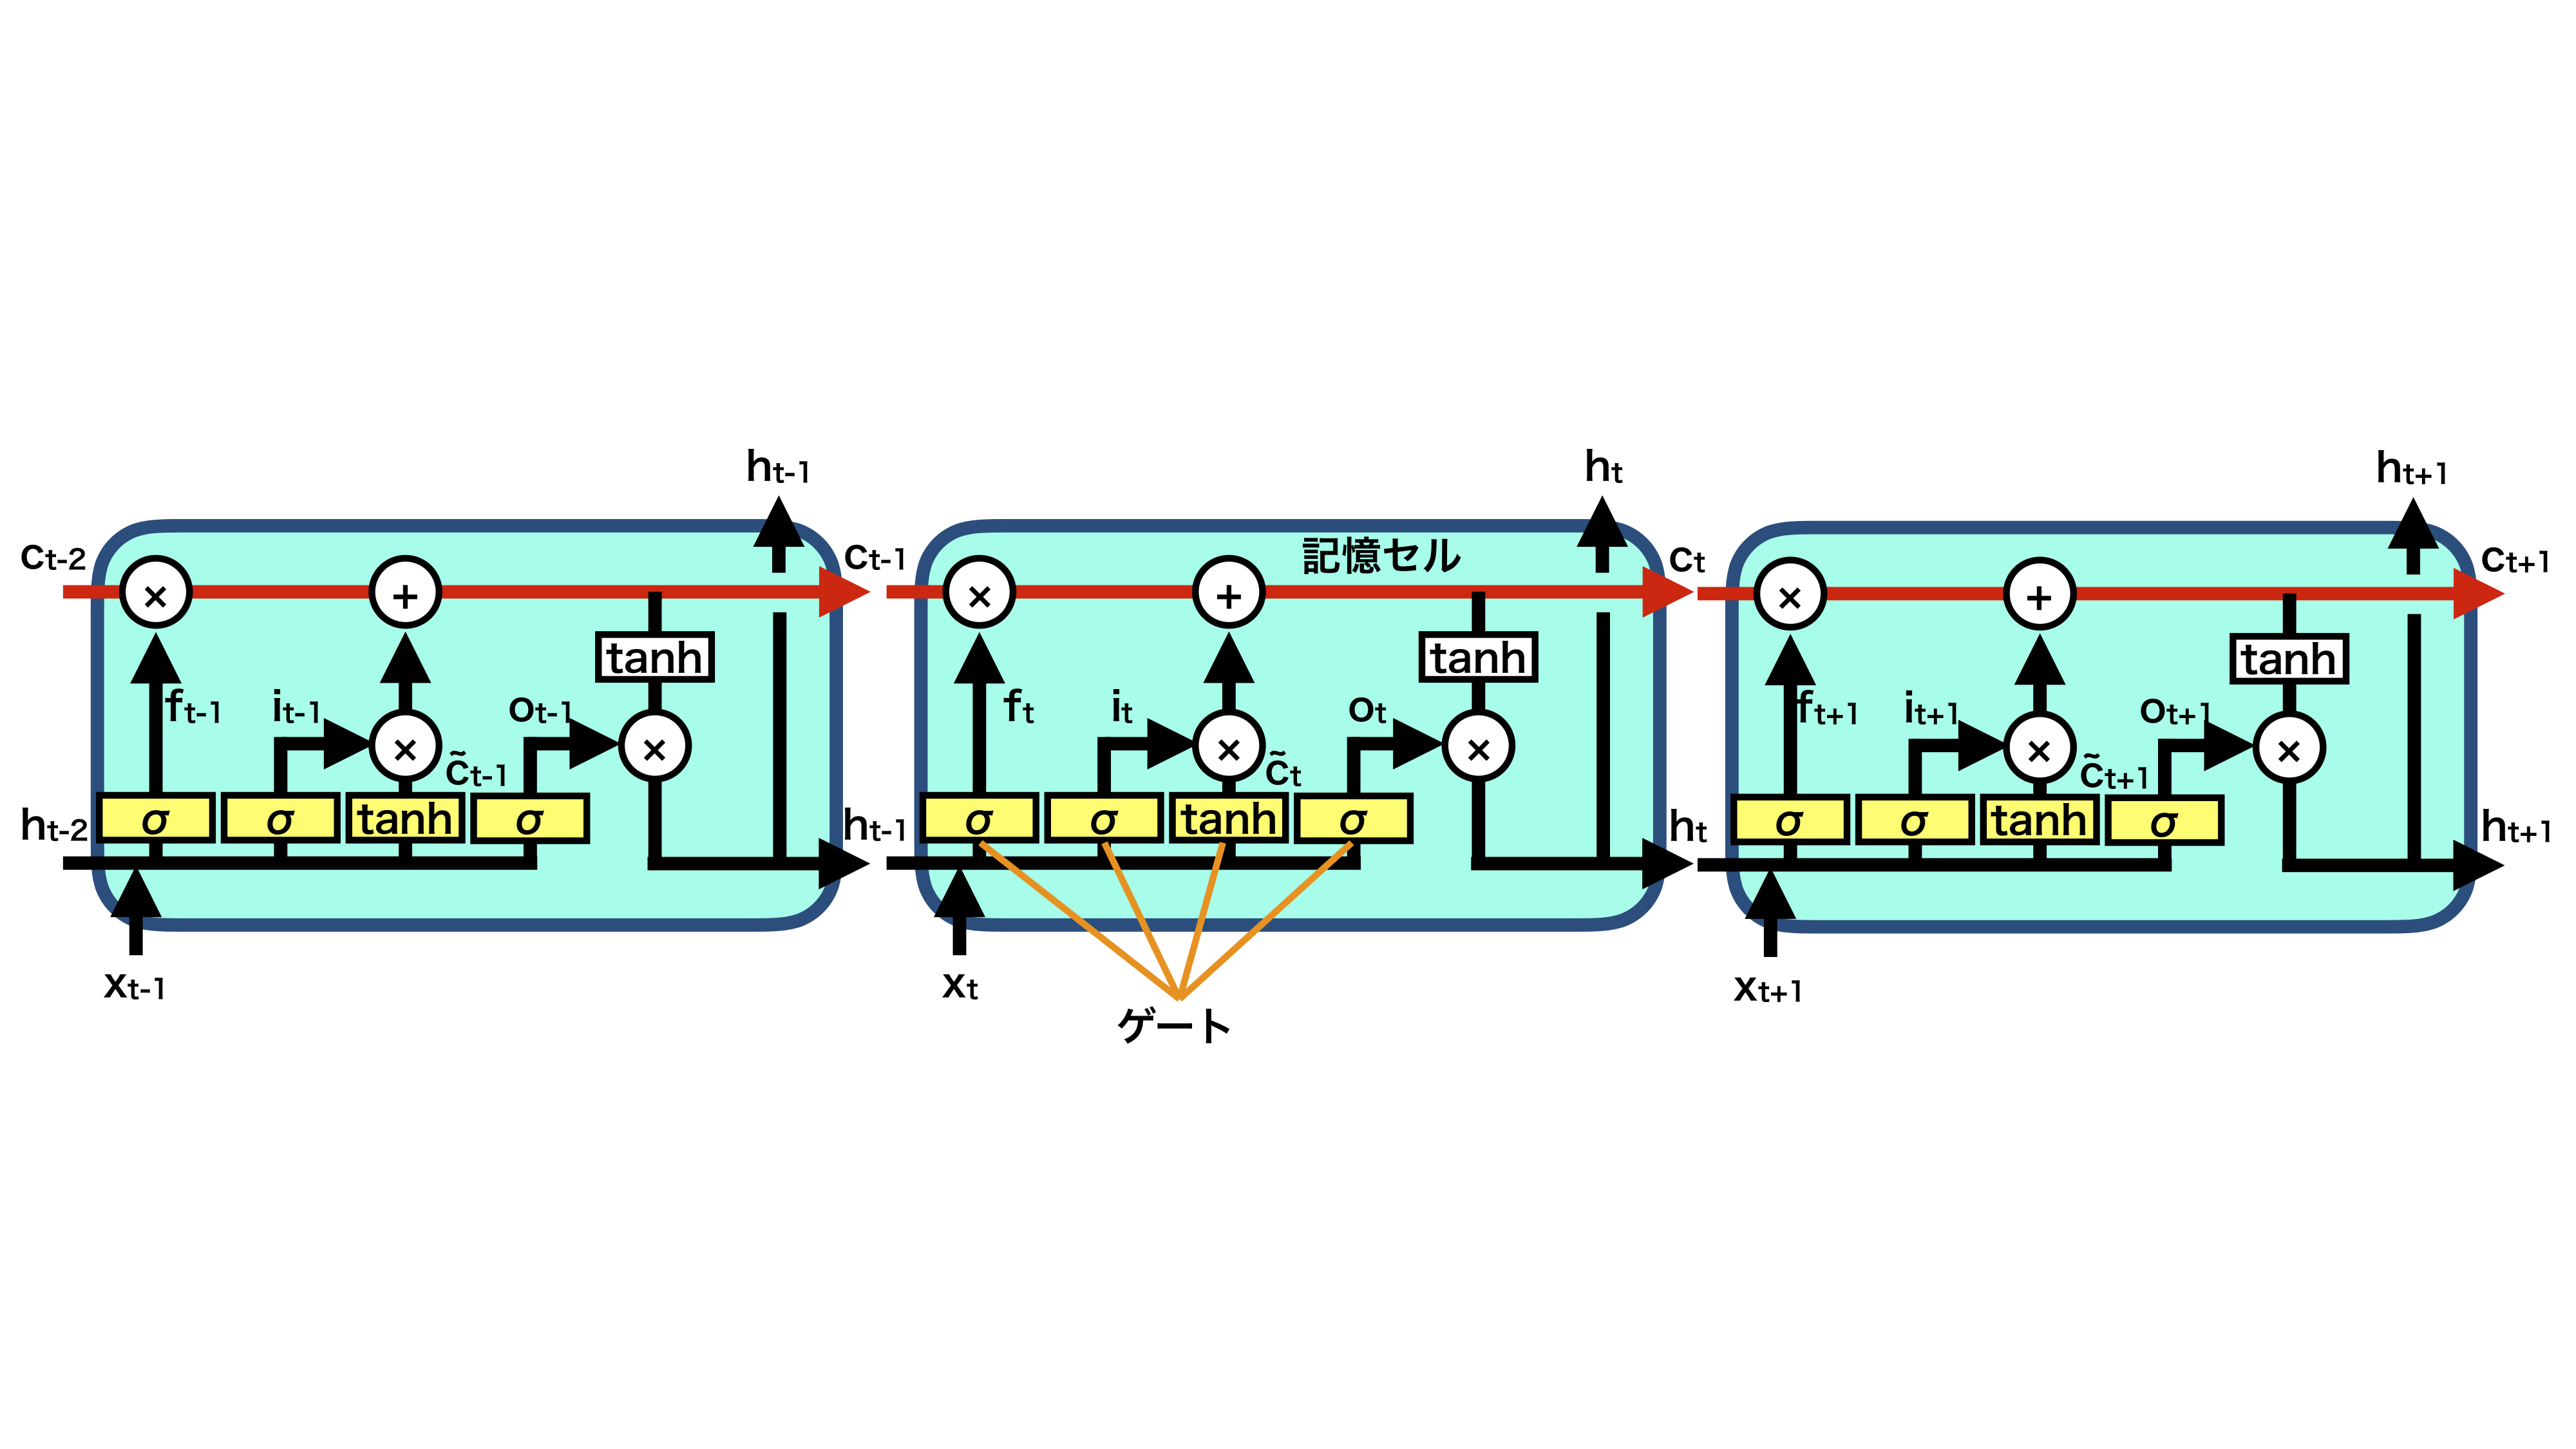
\includegraphics[trim = 0 200 0 200, width=1.0\textwidth, clip]{Figure/2DeepLearning/10LongShortTermMemory.png}
 \caption[LSTMの流れ]{LSTMの流れ。リカレントニューラルネットワークの様に時間について展開した図である。赤線が記憶セル, 黄色の各部がそれぞれゲートである。出力と隠れ状態である${\mbox{\boldmath{$h$}}},{\mbox{\boldmath{$c$}}}$は直前の系列から受け取り, 入力${\mbox{\boldmath{$x$}}}$は下方から導入されている。}
 \label{10LongShortTermMemory}
\end{figure}

また, LSTMは内部に前項で述べた勾配消失や勾配爆発, 入力重み衝突, 出力重み衝突といった様々な問題を解決するためのゲートと呼ばれる構造を四つ持っている(図\ref{10LongShortTermMemory})。

%\begin{comment}
\begin{figure}[htbp]
 \centering
 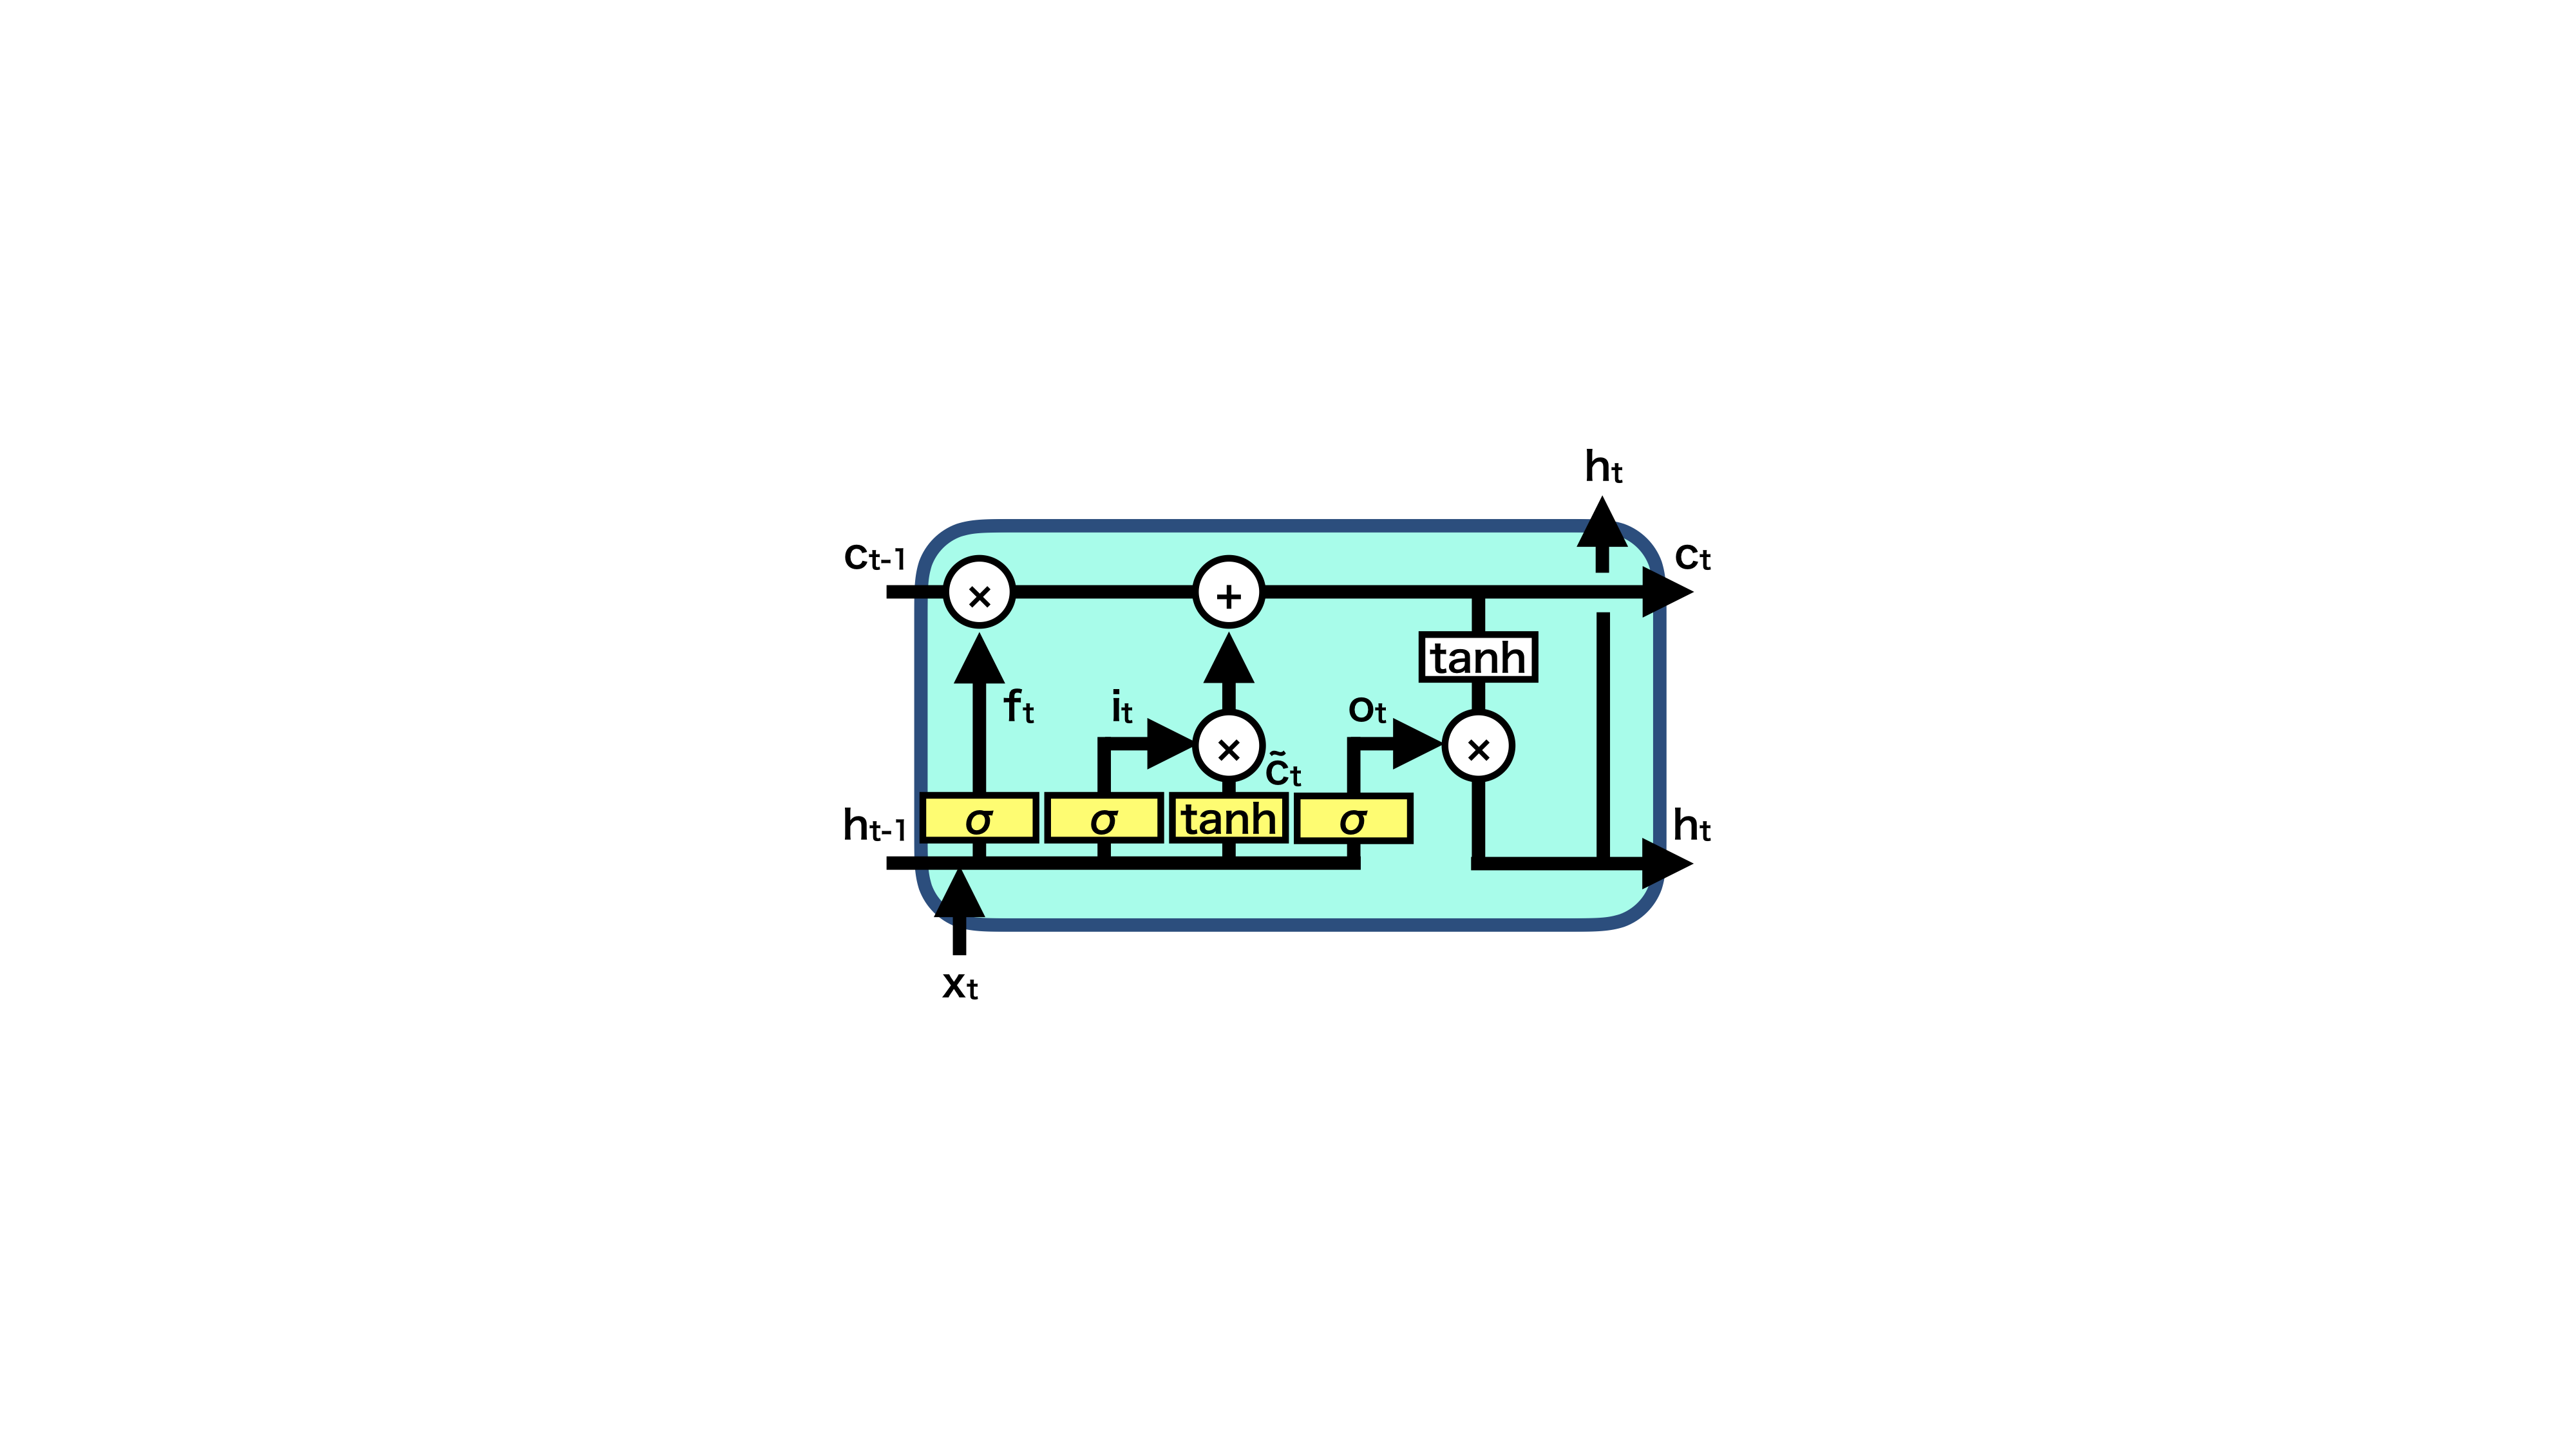
\includegraphics[trim = 0 300 0 300, width=1.0\textwidth, clip]{Figure/2DeepLearning/11LSTM.png}
 \caption[単体のLSTM]{単体のLSTM。系列$1$ステップ分のLSTMを切り出したものである。リカレントニューラルネットワークと同様に重み行列は各ステップに渡って同一のものが使用されている。}
 \label{11LSTM}
\end{figure}
%\end{comment}

四つのゲートはそれぞれ忘却ゲート, 入力ゲート, セルの更新, 出力ゲートと呼ばれている。
入力ゲート, 出力ゲートはそれぞれ重み衝突を回避するために導入されており, 忘却ゲート, セルの更新は長期記憶の適切な長期記憶セルの更新を行う為のアイデアである。
それぞれの役割と演算を以下にまとめる。

\begin{itemize}
  \item 忘却ゲート\\
  図\ref{12ForgetGate}の赤い線で表現している領域では, 入力${\mbox{\boldmath{$h$}}}_{t-1},{\mbox{\boldmath{$x$}}}_t$を用いて, どの程度, 直前の長期記憶セル${\mbox{\boldmath{$c$}}}_{t-1}$を忘れるかの度合いである${\mbox{\boldmath{$f$}}}_{t}$を計算している。
  ${\mbox{\boldmath{$f$}}}_{t}$は, 次のようにかける。
\begin{equation}
 \begin{split}
  {\mbox{\boldmath{$f$}}}_{t} = \sigma (W_f {\mbox{\boldmath{$x$}}}_t + R_f {\mbox{\boldmath{$h$}}}_{t-1})
 \end{split}
\end{equation}  
  したがって最終的には, 
\begin{equation}
 \begin{split}
  {\mbox{\boldmath{$c$}}}_{t-1} \  {\mbox{\boldmath{$f$}}}_{t} 
  = {\mbox{\boldmath{$c$}}}_{t-1} \  \sigma (W_f {\mbox{\boldmath{$x$}}}_t + R_f {\mbox{\boldmath{$h$}}}_{t-1})
 \end{split}
\end{equation}
  として, 次のゲート以降で長期記憶を更新するための容量を確保していると解釈できる。

  \item 入力ゲート\\
  入力ゲートは忘却ゲートと全く同じ構造 (図\ref{13InputGate}) をしており, 次のように計算できる。
\begin{equation}
 \begin{split}
  {\mbox{\boldmath{$i$}}}_{t} = \sigma (W_i {\mbox{\boldmath{$x$}}}_t + R_i {\mbox{\boldmath{$h$}}}_{t-1})
 \end{split}
\end{equation}
  忘却ゲートではどの程度, 長期記憶セルを忘れるかを計算していたように, 入力ゲートでの${\mbox{\boldmath{$i$}}}_{t}$は, 次のセルの更新時に新しい長期記憶セルをどの程度重視するかを表現していると解釈できる。
    
  \item セルの更新\\
  図\ref{14CellUpdate}では, まず更新された長期記憶セル$\tilde{{\mbox{\boldmath{$c$}}}}_t$を計算している。
\begin{equation}
 \begin{split}
  \tilde{{\mbox{\boldmath{$c$}}}}_t = \tanh (W_c {\mbox{\boldmath{$x$}}}_t + R_c {\mbox{\boldmath{$h$}}}_{t-1})
 \end{split}
\end{equation} 
  次にこれまでの三つのゲートの結果をまとめることで, 新しい隠れ状態である長期記憶セル${\mbox{\boldmath{$c$}}}_{t}$を計算できる。
\begin{equation}
 \begin{split}
  {\mbox{\boldmath{$c$}}}_{t} 
  &= {\mbox{\boldmath{$c$}}}_{t-1} \  {\mbox{\boldmath{$f$}}}_{t} + \tilde{\mbox{\boldmath{$c$}}}_{t}\ {\mbox{\boldmath{$i$}}}_{t}\\
  &= {\mbox{\boldmath{$c$}}}_{t-1} \  \sigma (W_f {\mbox{\boldmath{$x$}}}_t + R_f {\mbox{\boldmath{$h$}}}_{t-1}) 
  + \tanh (W_c {\mbox{\boldmath{$x$}}}_t + R_c {\mbox{\boldmath{$h$}}}_{t-1}) \  \sigma (W_i {\mbox{\boldmath{$x$}}}_t + R_i {\mbox{\boldmath{$h$}}}_{t-1})
 \end{split}
\end{equation}
  第一項では, 直前の長期記憶セル${\mbox{\boldmath{$c$}}}_{t-1}$をどの程度忘れるかを${\mbox{\boldmath{$f$}}}_{t}$によって制御し, 第二項では, 新しく計算された長期記憶セル$\tilde{\mbox{\boldmath{$c$}}}_{t}$をどの程度重視するかを${\mbox{\boldmath{$i$}}}_{t}$によって制御している。
    
  \item 出力ゲート\\
  出力ゲートでは, ここまでで計算された${\mbox{\boldmath{$c$}}}_{t}$と入力${\mbox{\boldmath{$x$}}}_t, {\mbox{\boldmath{$h$}}}_{t-1}$を用いて, 最終的な出力となる${\mbox{\boldmath{$h$}}}_{t}$を計算している。
  ただし, 出力ゲート${\mbox{\boldmath{$o$}}}_{t}$自体は入力ゲートや忘却ゲートと全く同じ形 (図\ref{15OutputGate}) をしている。
  具体的な計算は次のように書ける。
\begin{equation}
 \begin{split}
  {\mbox{\boldmath{$o$}}}_{t} 
  &= \sigma (W_o {\mbox{\boldmath{$x$}}}_t + R_o {\mbox{\boldmath{$h$}}}_{t-1})\\
  {\mbox{\boldmath{$h$}}}_{t} 
  &= \tanh({\mbox{\boldmath{$c$}}}_{t}) \  {\mbox{\boldmath{$o$}}}_{t}\\
  &= \tanh({\mbox{\boldmath{$c$}}}_{t}) \  \sigma (W_o {\mbox{\boldmath{$x$}}}_t + R_o {\mbox{\boldmath{$h$}}}_{t-1})\\
  &= \tanh({\mbox{\boldmath{$c$}}}_{t-1} \  \sigma (W_f {\mbox{\boldmath{$x$}}}_t + R_f {\mbox{\boldmath{$h$}}}_{t-1}) 
  + \tanh (W_c {\mbox{\boldmath{$x$}}}_t + R_c {\mbox{\boldmath{$h$}}}_{t-1}) \  \sigma (W_i {\mbox{\boldmath{$x$}}}_t + R_i {\mbox{\boldmath{$h$}}}_{t-1})) \\
  &\  \sigma (W_o {\mbox{\boldmath{$x$}}}_t + R_o {\mbox{\boldmath{$h$}}}_{t-1})
 \end{split}
\end{equation}
\end{itemize}

\begin{figure}[htbp]
 \centering
  %\begin{tabular}{cccc}
  \begin{minipage}{1.0\textwidth}
  \centering
   \begin{minipage}{0.48\textwidth}
    \centering
    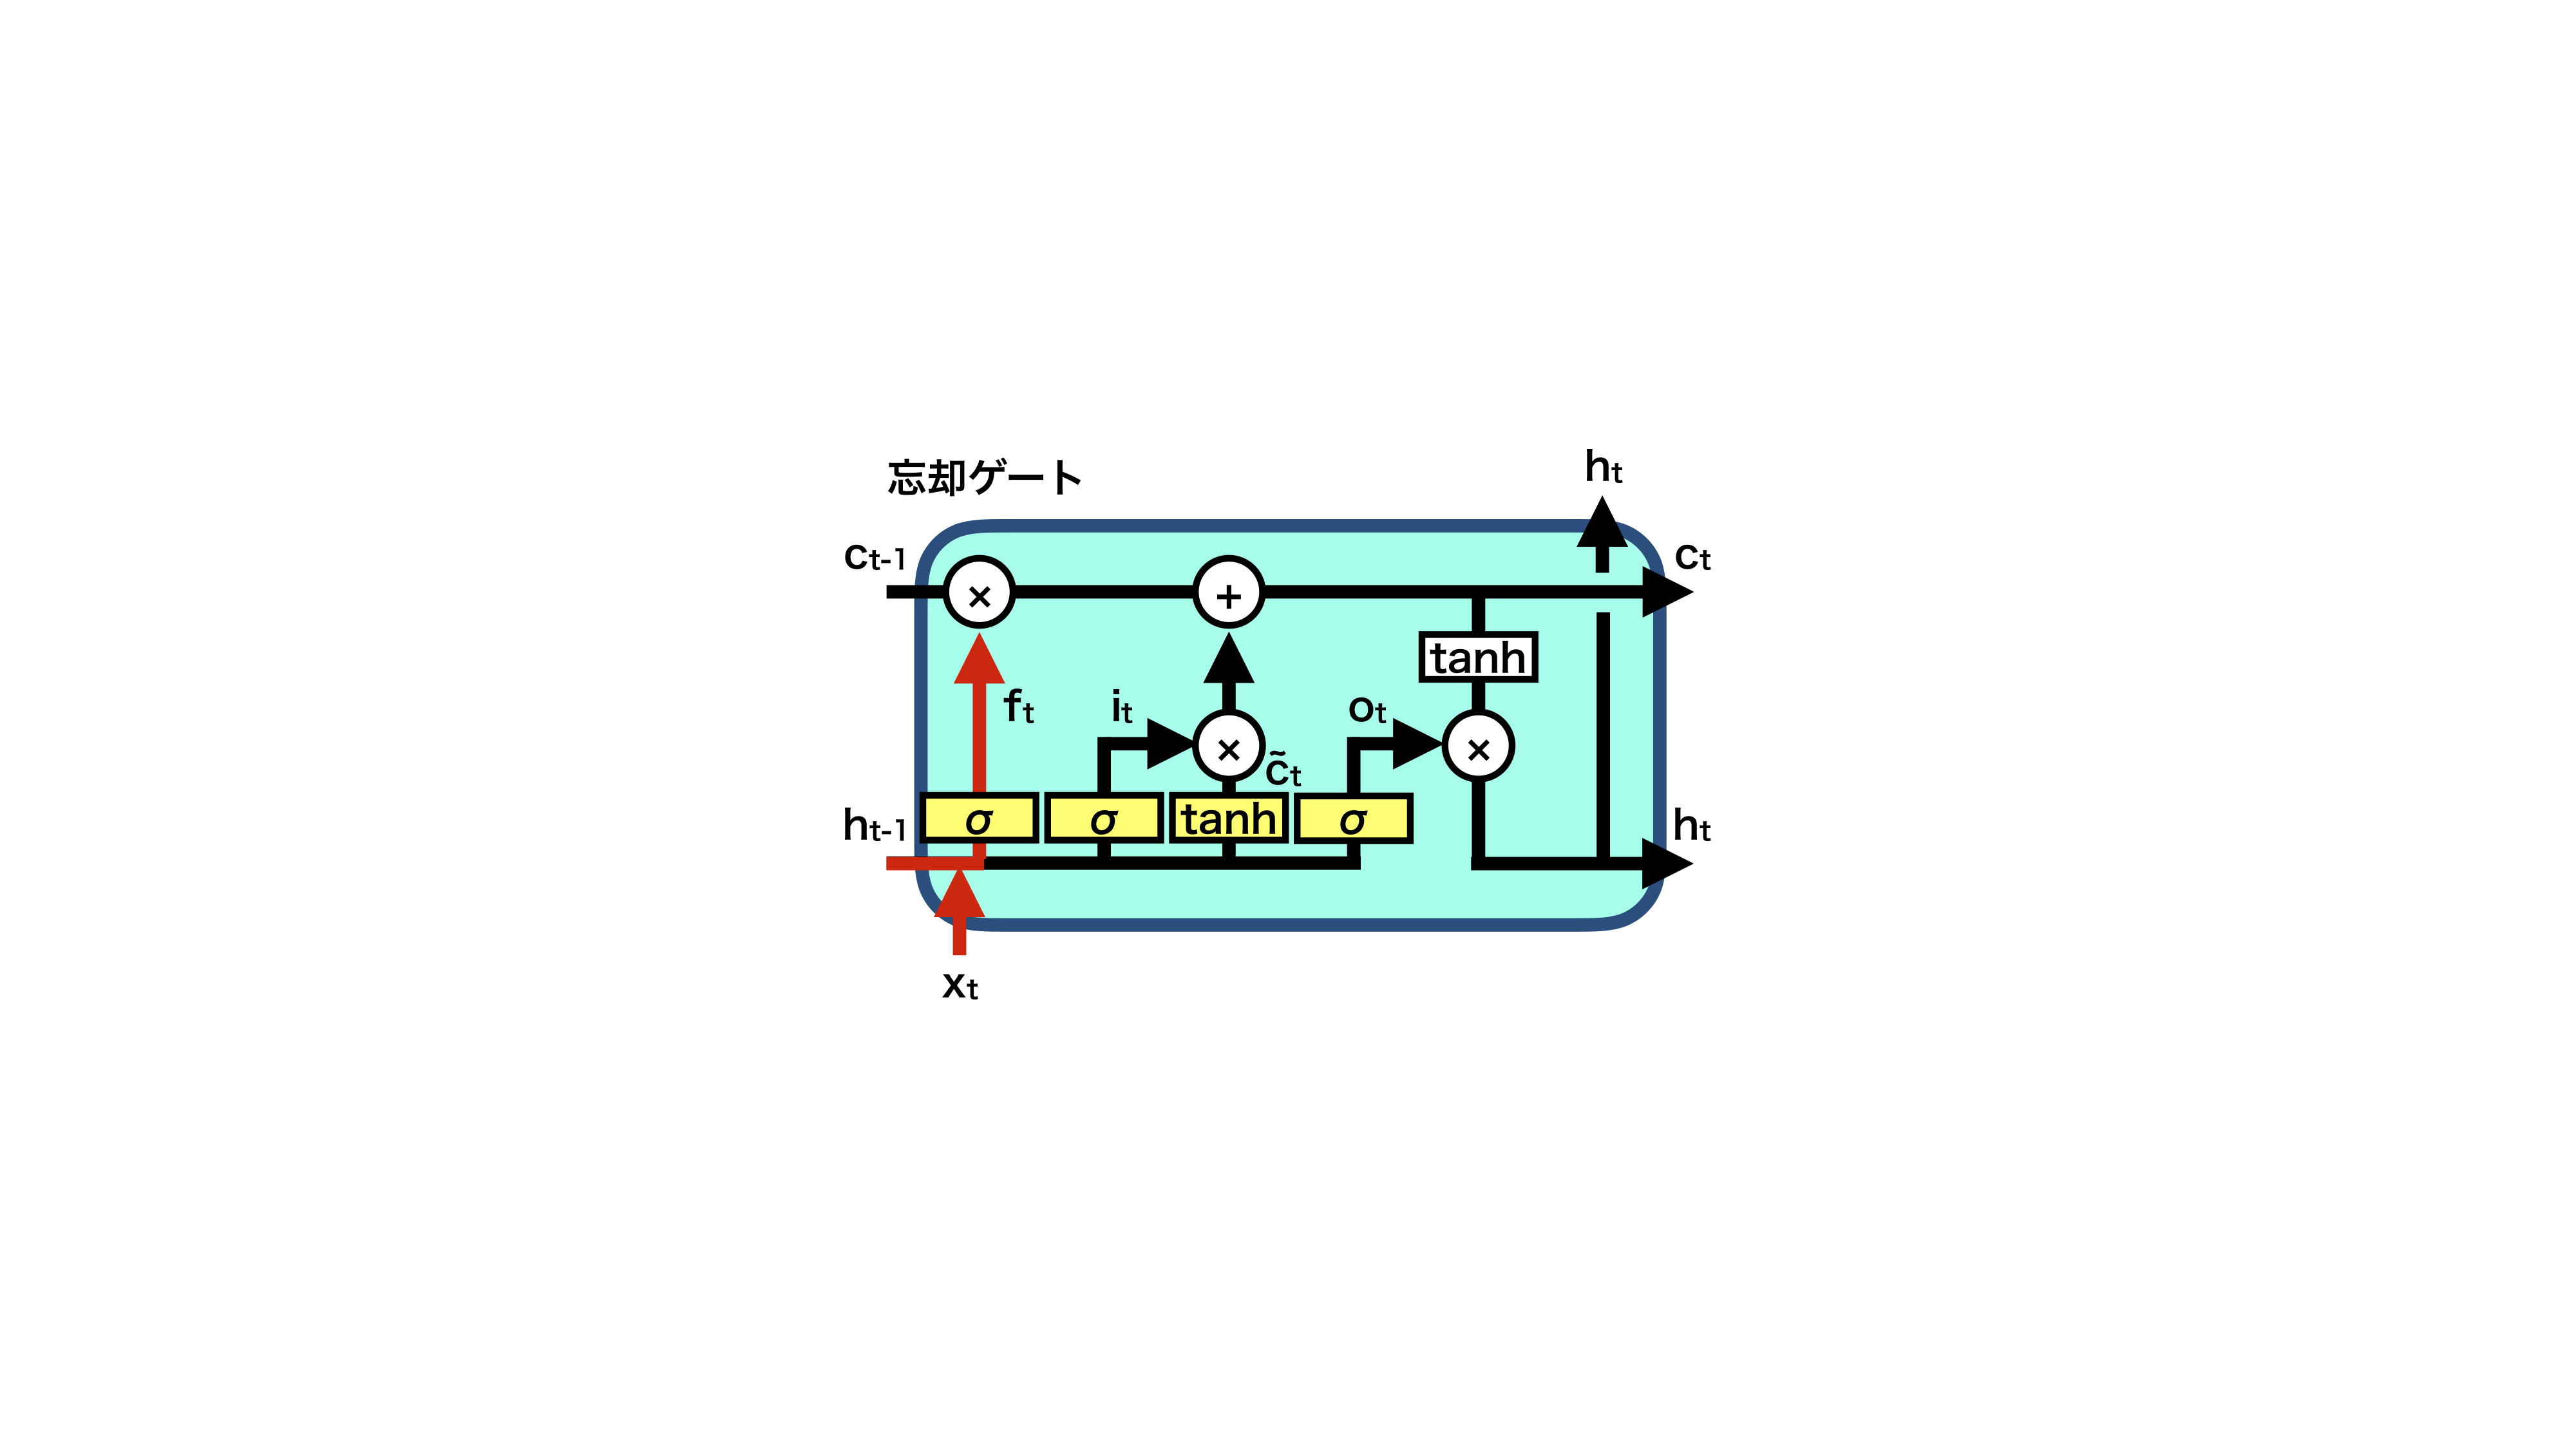
\includegraphics[trim = 600 300 600 300, width=0.9\textwidth, clip]{Figure/2DeepLearning/12ForgetGate.png}
    \subcaption{忘却ゲート}
    \label{12ForgetGate}
   \end{minipage}
   \begin{minipage}{0.48\textwidth}
   \centering
    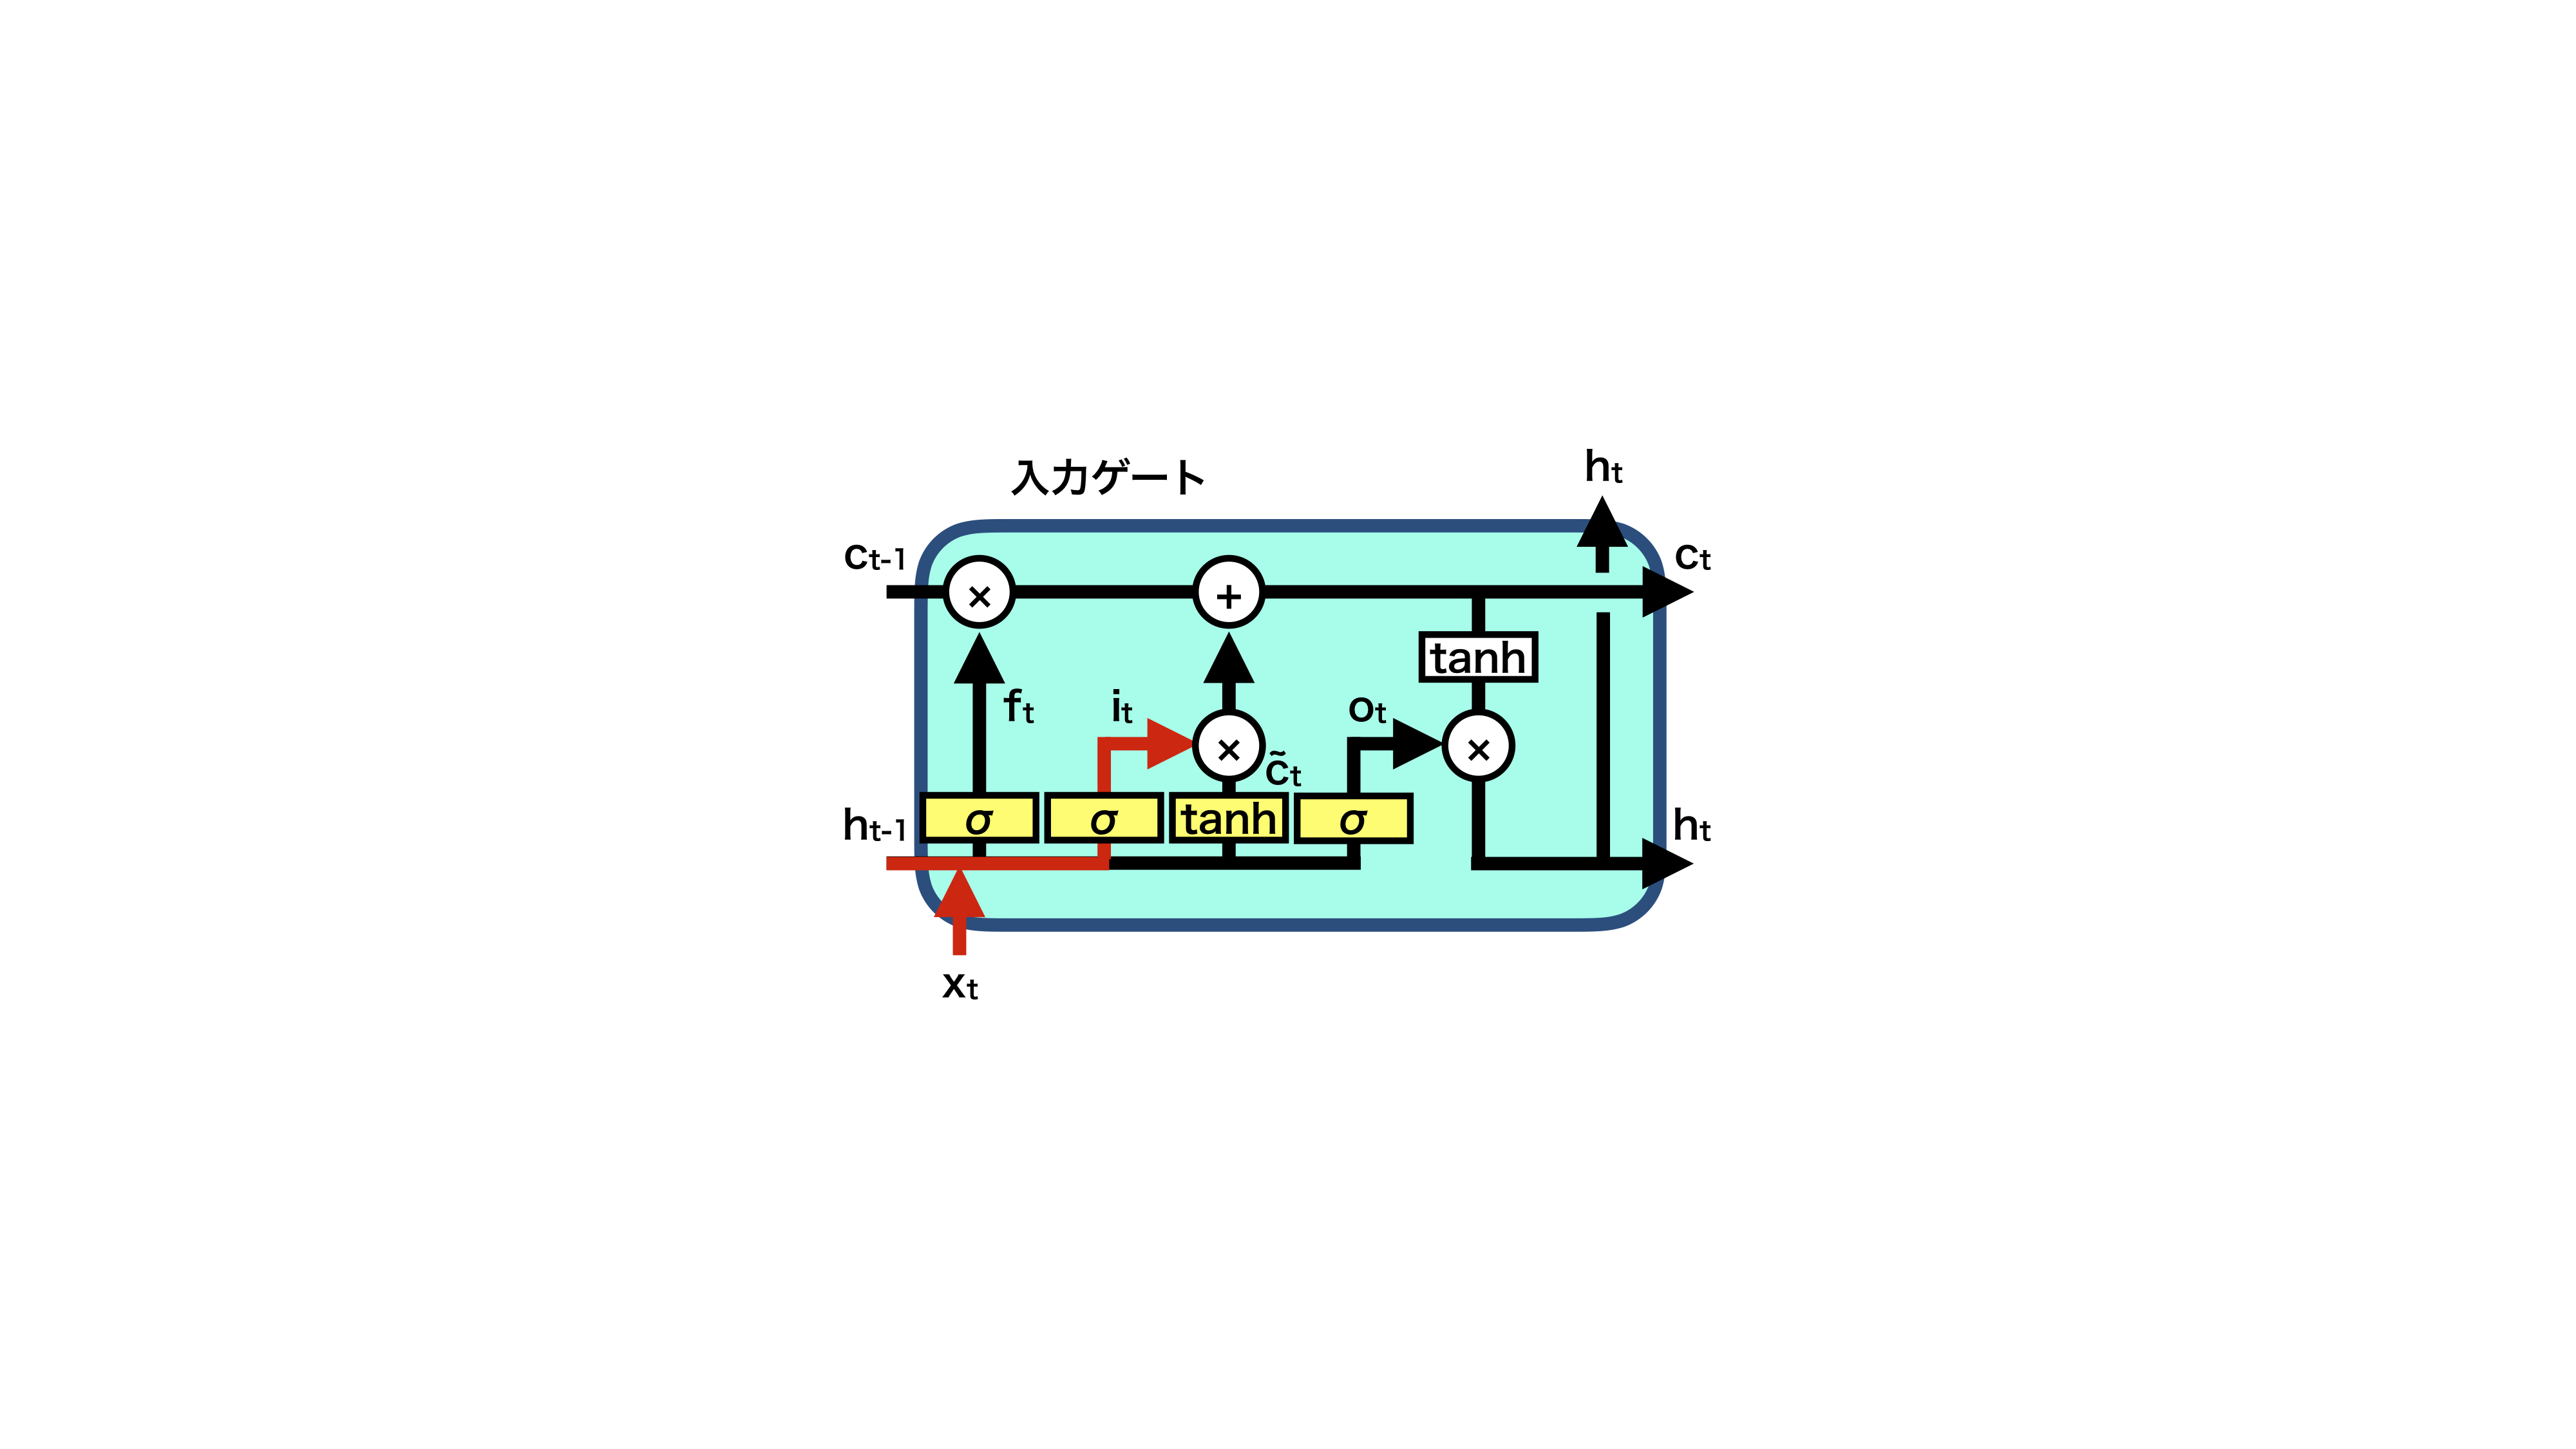
\includegraphics[trim = 600 300 600 300, width=0.9\textwidth, clip]{Figure/2DeepLearning/13InputGate.png}
    \subcaption{入力ゲート}
    \label{13InputGate}
   \end{minipage}
  \end{minipage}
  
  \begin{minipage}{1.0\textwidth}
  \centering
   \begin{minipage}{0.48\textwidth}
   \centering
    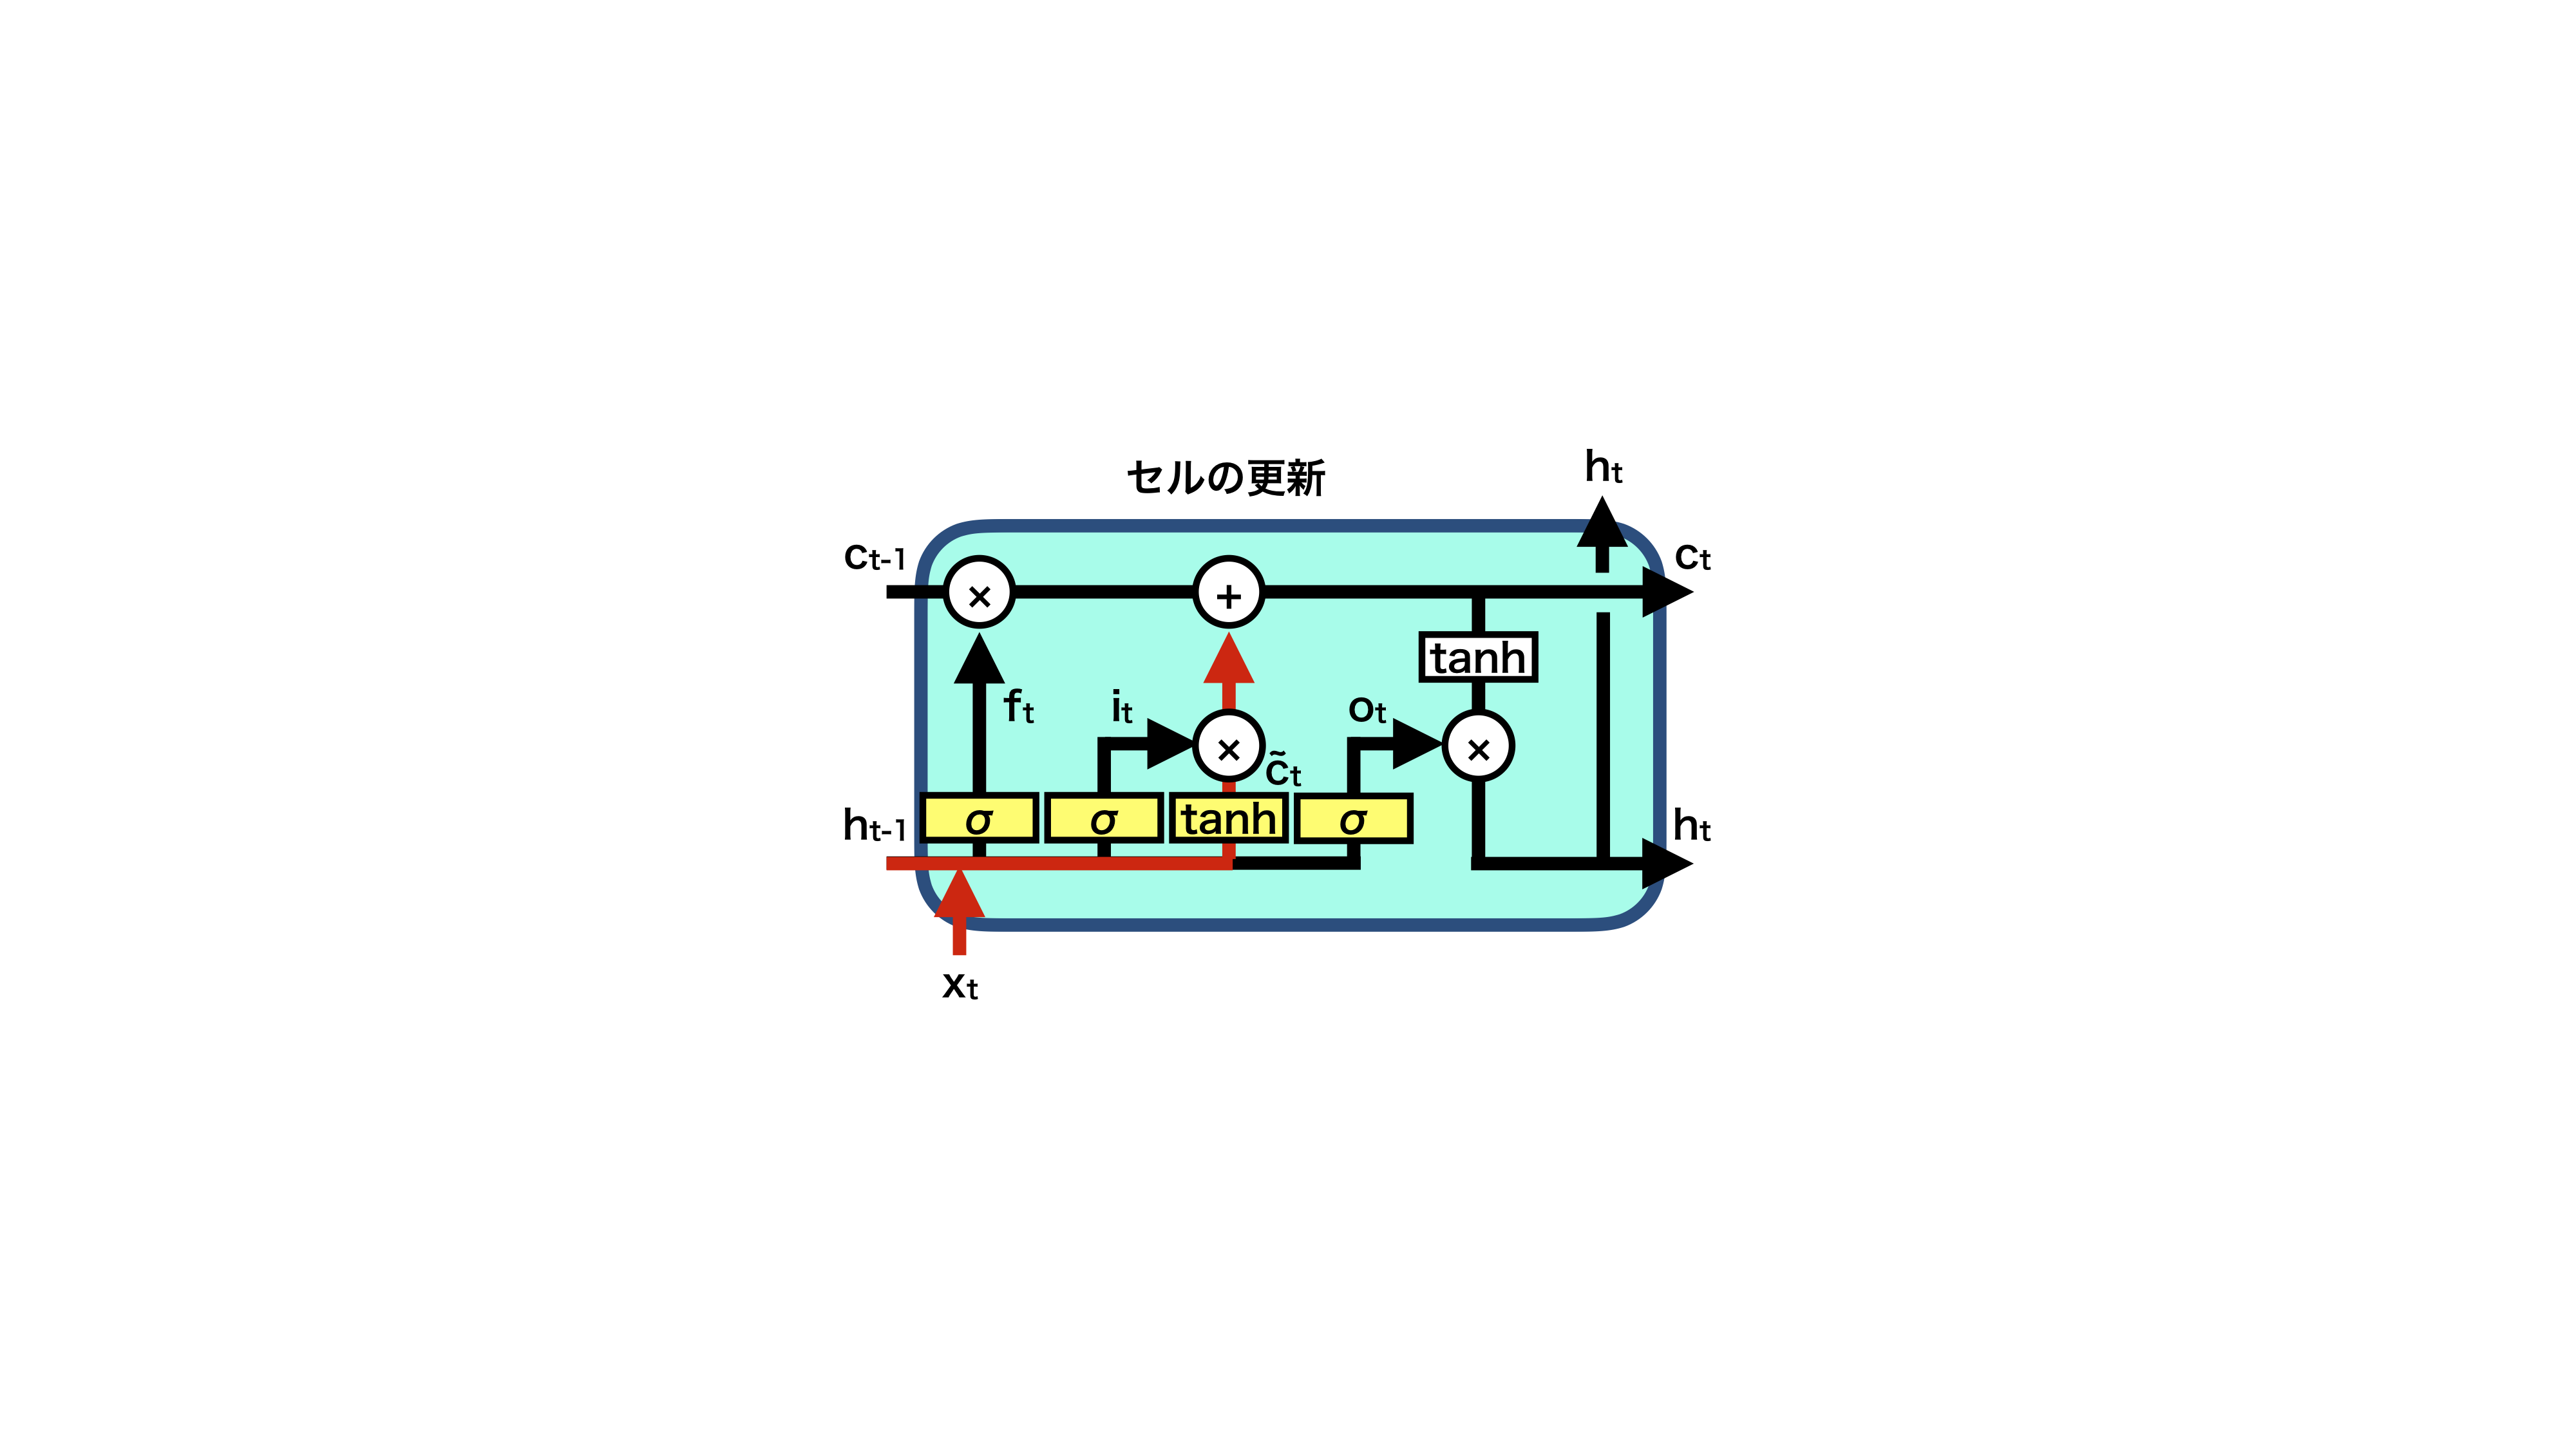
\includegraphics[trim = 600 300 600 300, width=0.9\textwidth, clip]{Figure/2DeepLearning/14CellUpdate.png}
    \subcaption{セルの更新}
    \label{14CellUpdate}
   \end{minipage}
   \begin{minipage}{0.48\textwidth}
   \centering
    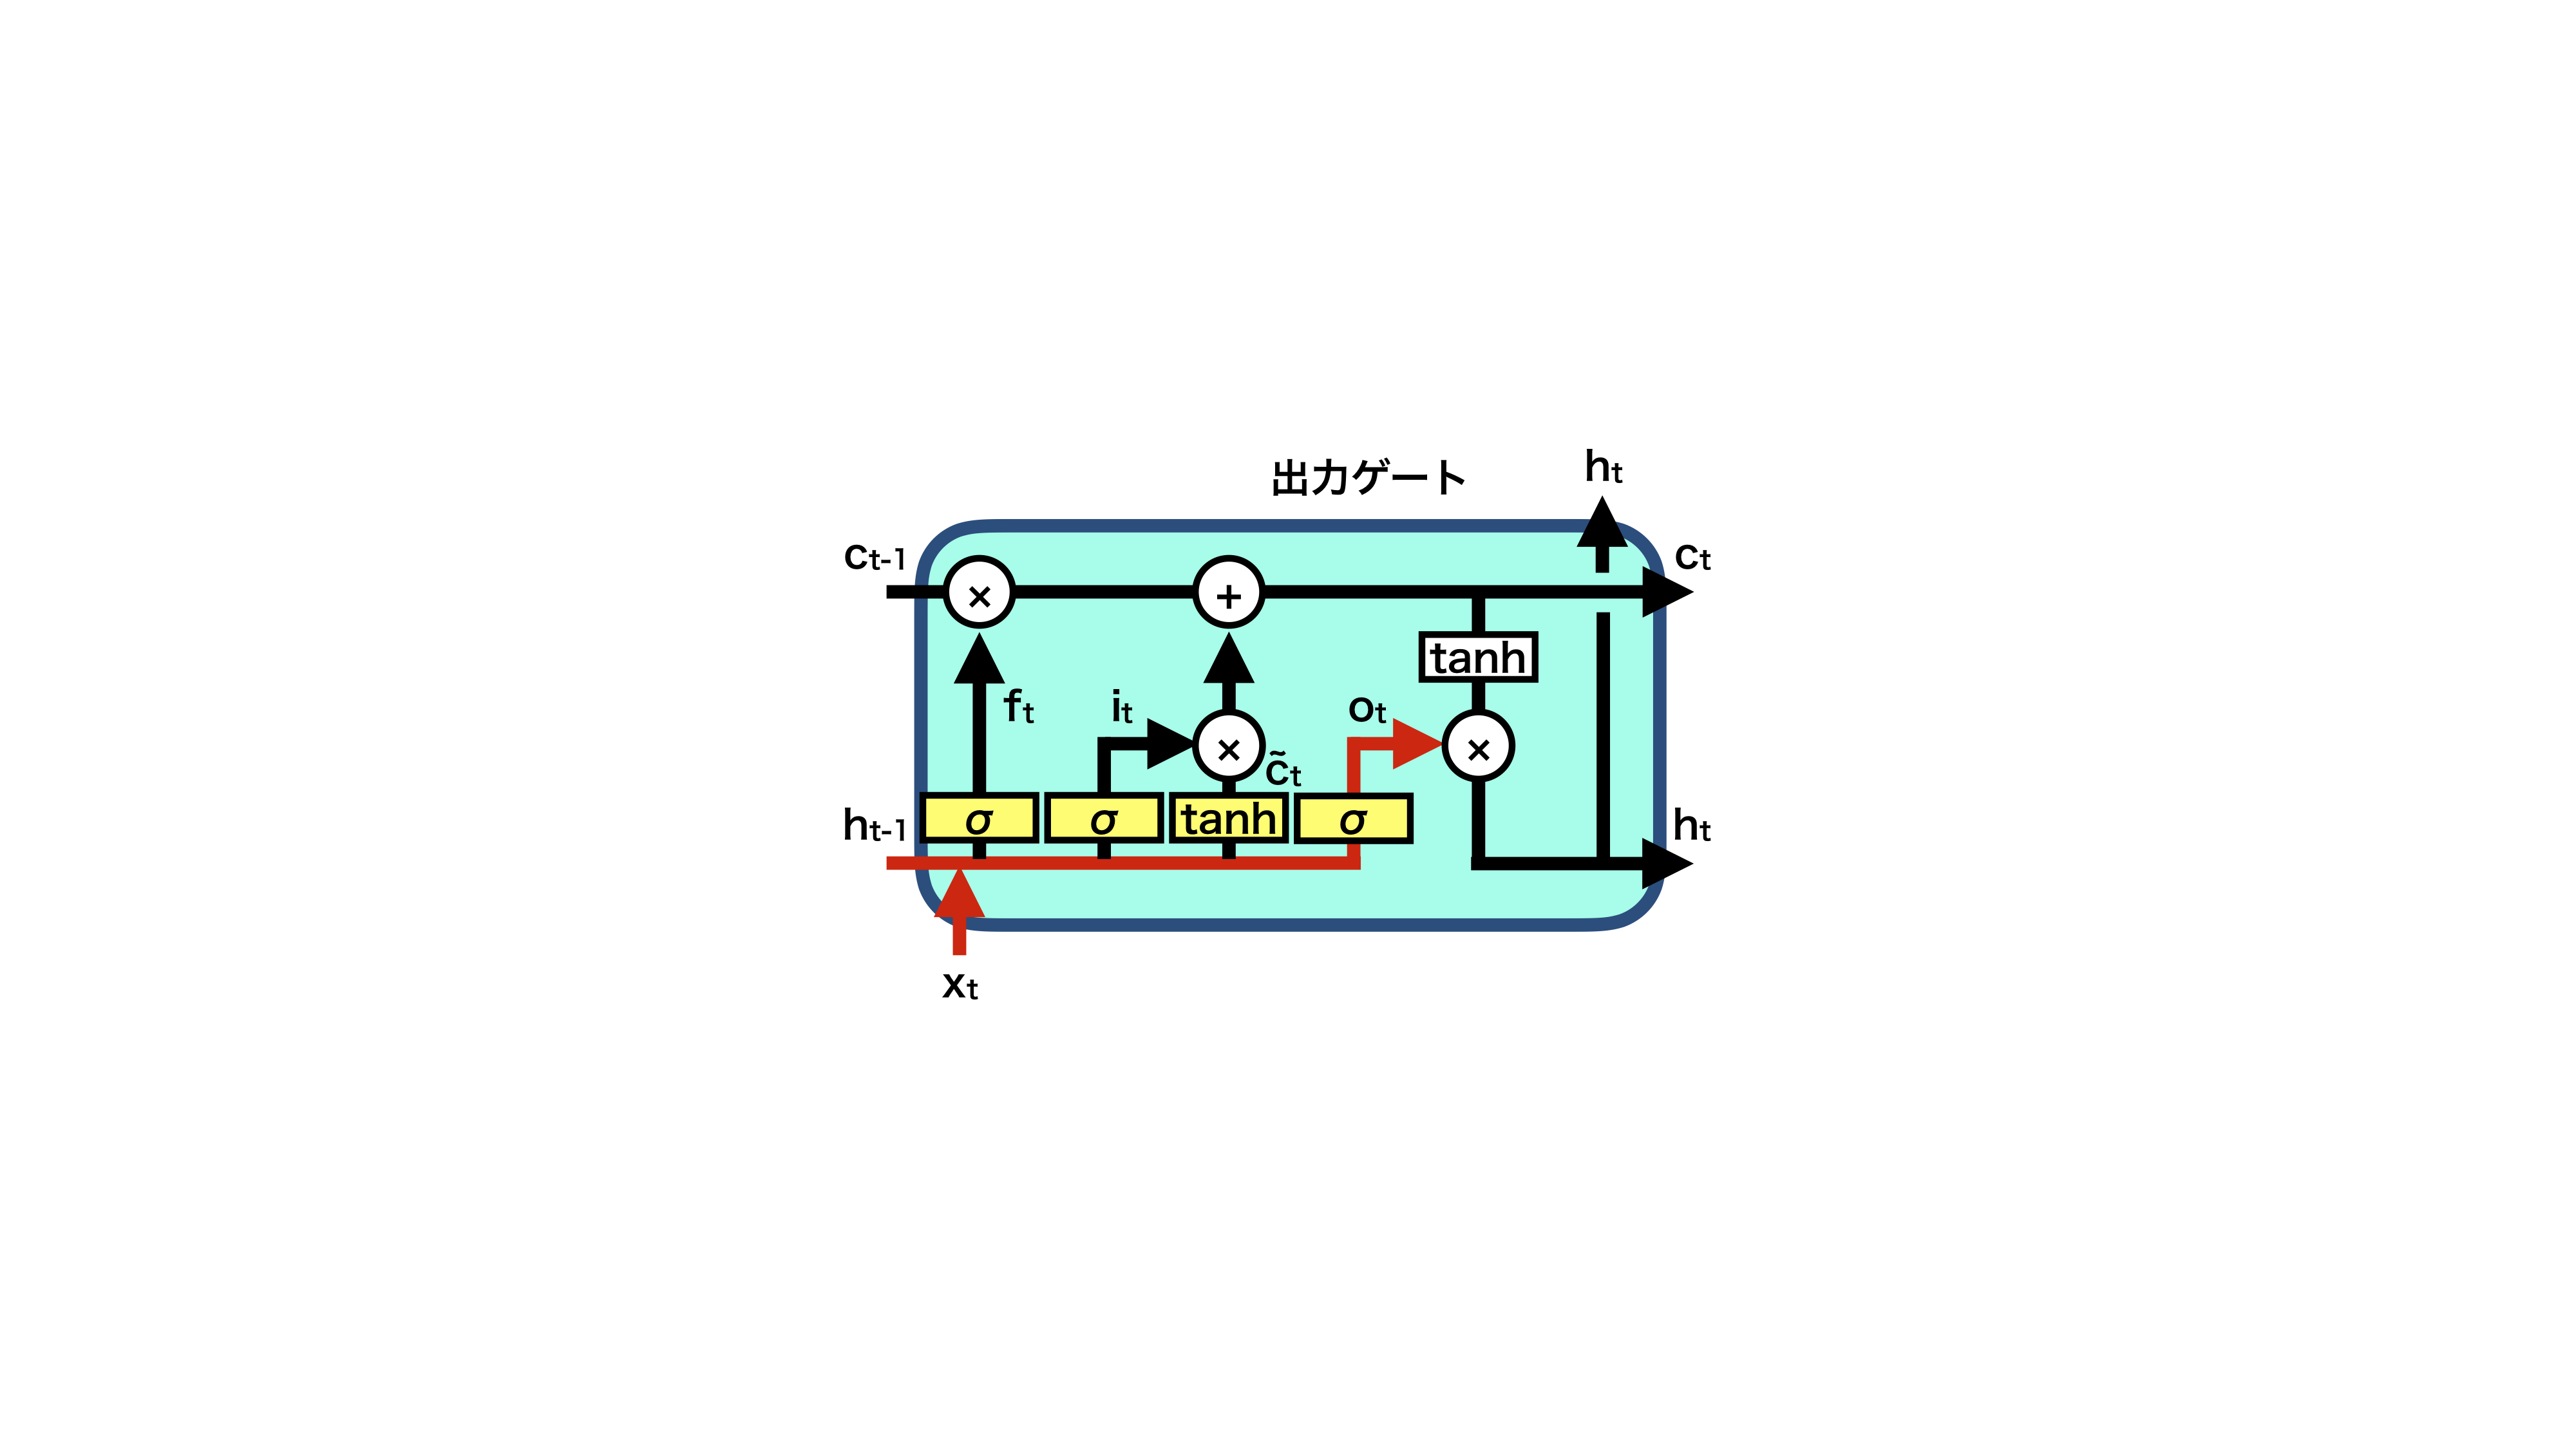
\includegraphics[trim = 600 300 600 300, width=0.9\textwidth, clip]{Figure/2DeepLearning/15OutputGate.png}
    \subcaption{出力ゲート}
    \label{15OutputGate}
   \end{minipage}
   \end{minipage}
  \caption[LSTMの各ゲートについての図解]{LSTMの各ゲートについての図解。それぞれ赤線部に沿って情報が伝達される。}
 %\end{tabular}
\end{figure}

以上のように, LSTMの内部構造は煩雑であるが, その構成要素は全てリカレントニューラルネットワークと同様に全結合で計算できる。
以下に最終的な出力の計算についてまとめる。
\begin{equation}
 \begin{split}
  {\mbox{\boldmath{$c$}}}_{t} 
  &= {\mbox{\boldmath{$c$}}}_{t-1} \  \sigma (W_f {\mbox{\boldmath{$x$}}}_t + R_f {\mbox{\boldmath{$h$}}}_{t-1}) 
  + \tanh (W_c {\mbox{\boldmath{$x$}}}_t + R_c {\mbox{\boldmath{$h$}}}_{t-1}) \  \sigma (W_i {\mbox{\boldmath{$x$}}}_t + R_i {\mbox{\boldmath{$h$}}}_{t-1})\\
  {\mbox{\boldmath{$h$}}}_{t} 
  &= \tanh({\mbox{\boldmath{$c$}}}_{t-1} \  \sigma (W_f {\mbox{\boldmath{$x$}}}_t + R_f {\mbox{\boldmath{$h$}}}_{t-1}) 
  + \tanh (W_c {\mbox{\boldmath{$x$}}}_t + R_c {\mbox{\boldmath{$h$}}}_{t-1}) \  \sigma (W_i {\mbox{\boldmath{$x$}}}_t + R_i {\mbox{\boldmath{$h$}}}_{t-1})) \\
  &\  \sigma (W_o {\mbox{\boldmath{$x$}}}_t + R_o {\mbox{\boldmath{$h$}}}_{t-1})
 \end{split}
\end{equation}

ここで, 隠れ状態 (出力) ${\mbox{\boldmath{$h$}}}_t,{\mbox{\boldmath{$c$}}}_t$の計算は全て入力${\mbox{\boldmath{$h$}}}_{t-1},{\mbox{\boldmath{$c$}}}_{t-1},{\mbox{\boldmath{$x$}}}_t$によって計算できている。
また, 学習可能な重み行列は$W_f, W_i, W_c, W_o, R_f, R_i, R_c, R_o$の八つである。
一般に, 適宜バイアス$b$が加えられる。

リカレントニューラルネットワークやLSTMは更に重ねられる (Stacked) という非常に強力な性質を持っている。
そのようなネットワークを図\ref{16StackedLSTM}に示す。
図からわかるように, 一段目のLSTMの出力が二段目のLSTMの入力になっている。
一方で, セルは両者で共有されず, 独立した状態を保持している。
それら以外の基本的な構造は一段であった時のLSTMと変わっていない。
このように, LSTMは系列としての深さだけでなく, フィードフォワードニューラルネットワークと同様に重ねることによる深さの確保が可能である。
勿論この重ねる操作は二段以上への拡張が可能であり, その場合は二段目の出力を三段目の入力に使うことによって実現できる。
どの程度重ねるかはハイパーパラメータである。

\begin{figure}[htbp]
 \centering
 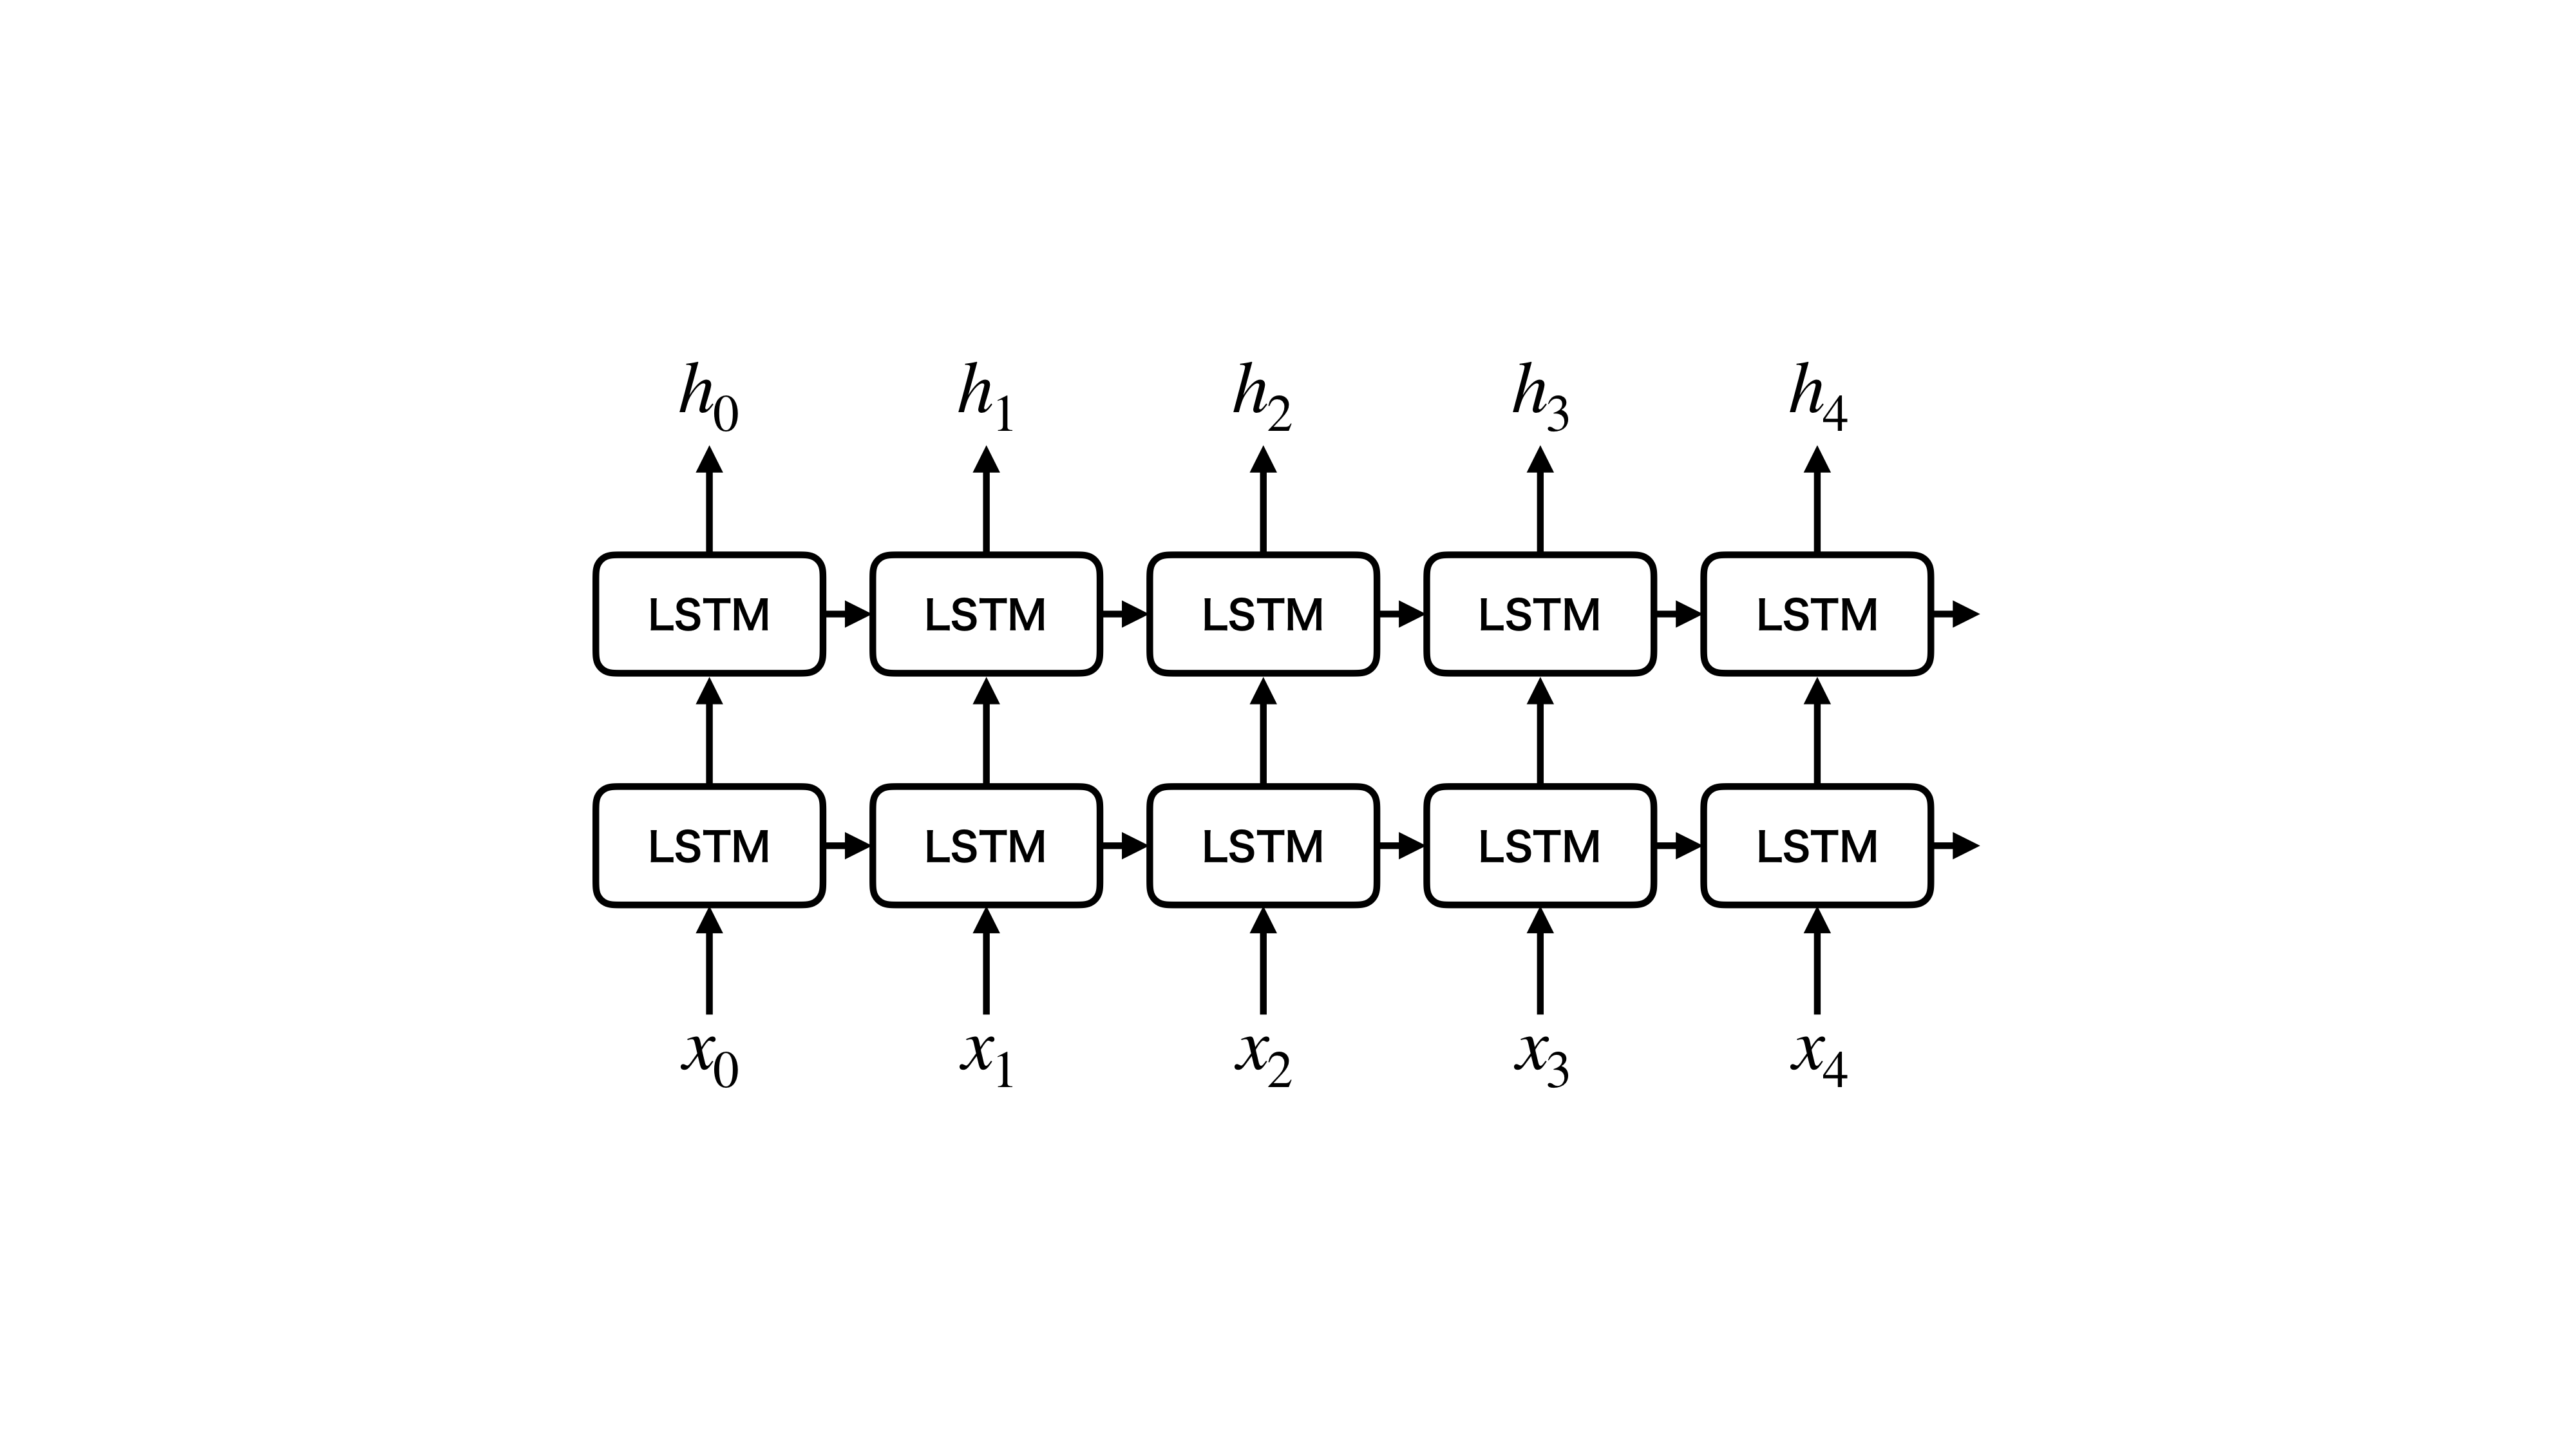
\includegraphics[trim = 0 200 0 200, width=1.0\textwidth, clip]{Figure/2DeepLearning/16StackedLSTM.png}
 \caption[Stacked LSTM]{Stacked LSTM。ここではLSTMの二つの隠れ状態を一つの線で表現している。下方を一段目, 上方を二段目と呼ぶと, 一段目の入力${\mbox{\boldmath{$x$}}}$と比べ, 一段目の出力・二段目の入力はより抽象度の高い情報となっている。}
 \label{16StackedLSTM}
\end{figure}

更に, 双方向 (Bidirectional) LSTMと呼ばれるネットワークに関しても解説する。
これは, 図\ref{17BidirectionalLSTM}のように, 片側を順方向に, もう一方を逆方向に系列を読み込むことにより, 自然言語処理などに見られる, 将来的な系列情報への依存を導入することができる。
ここで, 前述のLSTMを重ねる手法と異なり, それぞれのLSTMの入力はそれぞれ独立しており, 前段の出力を使用していないことに注意が必要である。
また, この双方向LSTMの構造上の性質として, 系列データを全て持っておく必要があるという点にも留意しなければならない。
したがって, リアルタイムな問題については, 未来の情報を得ることができない為, この双方向LSTMを用いることはできない。
また, この双方向LSTMを重ねることも可能である。

リカレントニューラルネットワークはこのように次々と拡張され, より複雑で難解な系列情報の処理について, 高い性能を発揮している。

\begin{figure}[htbp]
 \centering
 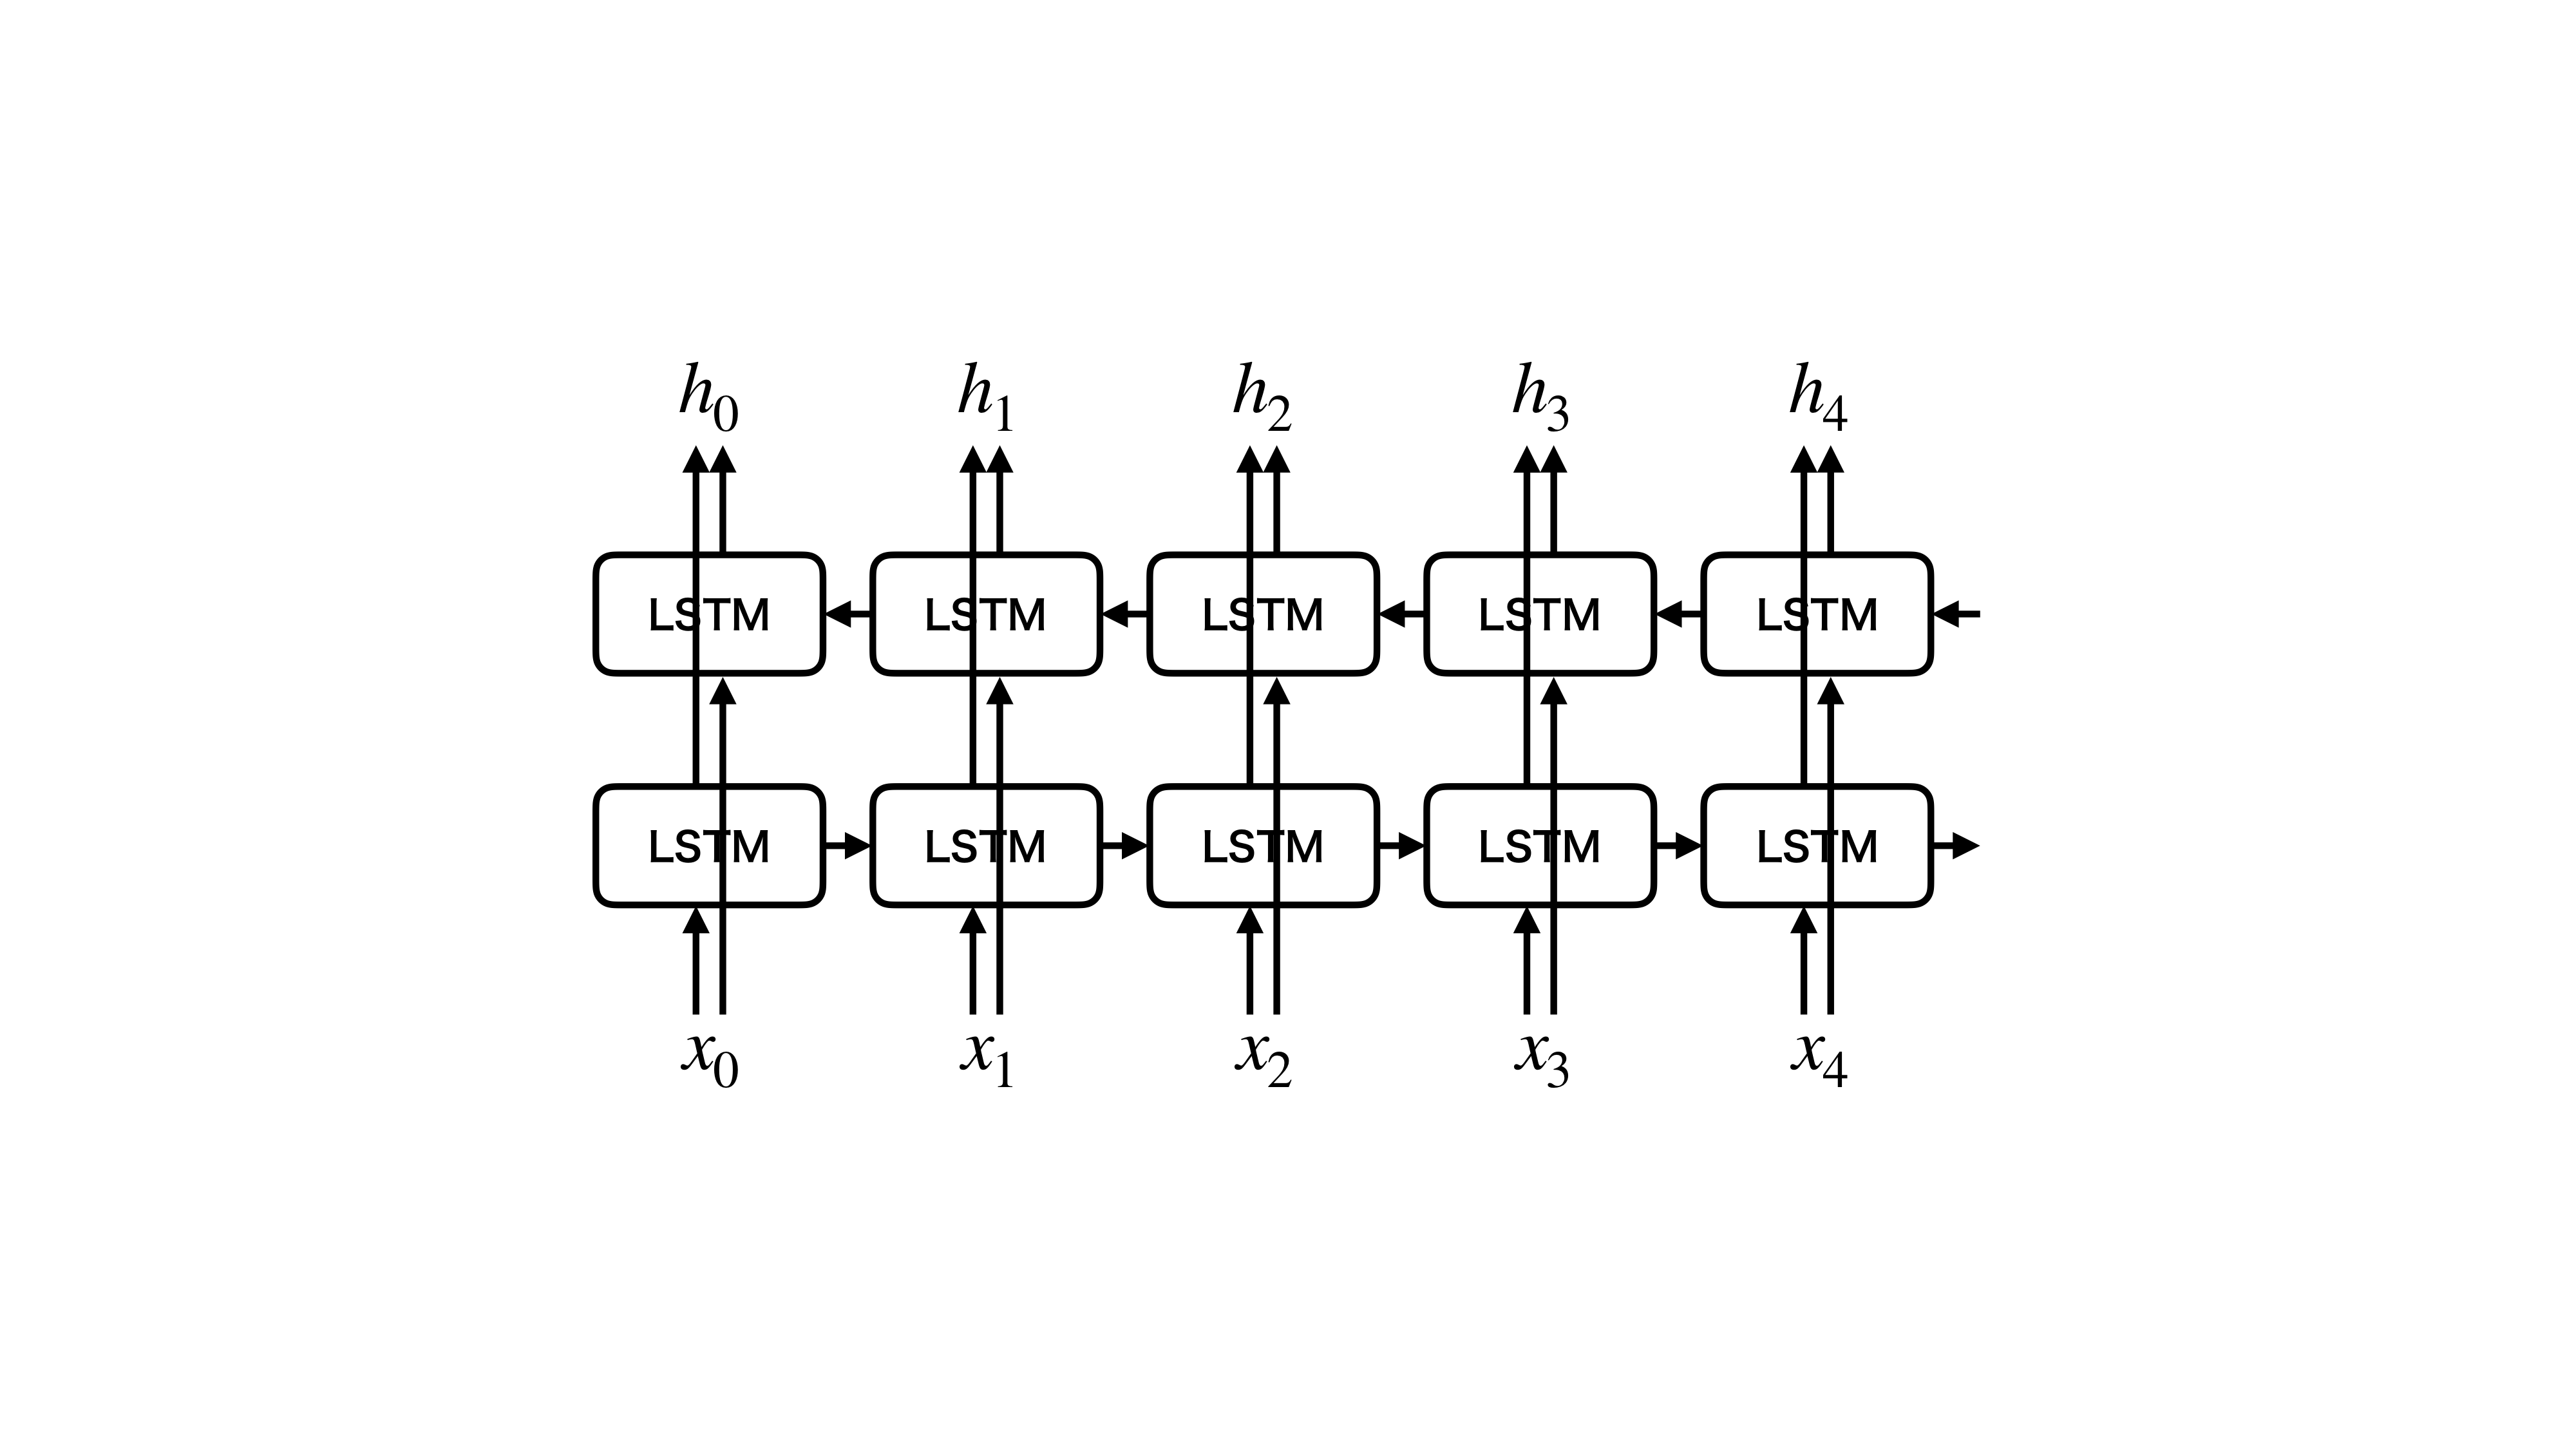
\includegraphics[trim = 0 200 0 200, width=1.0\textwidth, clip]{Figure/2DeepLearning/17BidirectionalLSTM.png}
 \caption[双方向LSTM]{双方向LSTM。Stacked LSTMとは異なり, 一段目のLSTMの出力は二段目の入力に使用されておらず, 計算はそれぞれ並列的に行われる。よって出力はLSTM二つ分の大きさになっている。}
 \label{17BidirectionalLSTM}
\end{figure}

リカレントニューラルネットワークはその構造が再帰的であるという点 (並列化が困難である) から, 学習が遅く, 重いという課題を抱えている。
また, 後述するエンコーダー・デコーダーモデルにおいては, データの系列の長さに応じた情報を確保できないという欠点が存在している。
\footnote{例えば, 機械翻訳を用いて$100$単語分の英文を日本語に翻訳する場合と$10$単語分の英文を翻訳する場合において, $100$単語分の英文が持つ情報の方が$10$単語分の英文と比べて多いことは明らかであるが, リカレントニューラルネットワークはこれらの情報の多さの違いに対応できず, 常に同じ量の情報から日本語を生成してしまう。}
次節では, このような問題を解決するための注意機構 (Attention) という技術を解説する。


%%%%%%%%%%%%%%%%%%%%%%%%%%%%%%%%%%%%%%%%%%%%%%%%%%%%%%%%%%%%%%%%%%%%%%%%%%%%%%%%%%%%%%%%%%%%%%%%%%%%%
\section{Attention} \label{DL:Attention}

Attention\cite{BahdanauAttention, LuongAttention}はその名の通り, ある系列データのどこに注意するかを計算する機構である。
主に機械翻訳や意味理解などのエンコーダー・デコーダーモデルに使用されており, 様々な応用が議論されているが, ここでは基本的なAttentionの理論と考え方についてのみ解説する。

\ref{DL:Atten:EncoderDecoderModel}項では, まずAttentionを理解する上で必要不可欠なエンコーダー・デコーダーモデルについて述べ, その中で前節のリカレントニューラルネットワークが抱える問題について紹介する。
次に, \ref{DL:Atten:Attention}項でAttentionの理論や計算について述べる。


%%%%%%%%%%%%%%%%%%%%%%%%%%%%%%%%%%%%%%%%%%%%%%%%%%%%%%%%%%%%%%%%%%%%%%%%
\subsection{エンコーダー・デコーダーモデル} \label{DL:Atten:EncoderDecoderModel}

Attentionは主に機械翻訳などのエンコーダー・デコーダーモデルに使用されている。
LSTMを用いたエンコーダー・デコーダーモデルの大まかな構成を図\ref{18EncoderDecoderLSTM}に示す。
LSTMではエンコーダーとデコーダーを繋ぐ情報はエンコーダーの最後の層の出力を使用することが多い。
つまり, エンコーダーは図\ref{9RNNOutputs}のMany to One, デコーダーはOne to Manyを使用しており, エンコーダーによって抽出された情報はこのOneの部分に集められることになる。
この出力はMany to Oneの内, Manyであるデータの系列の長さ (系列長) に依存せず, 常に同じ大きさとなる。
これは長い系列長であっても, 短い系列長であっても同じ量の情報を使用しているということを意味している。
したがって, より長い系列長や短い系列長を扱う場合は, そのデータが持つ情報を完全に保持, 表現することは難しく, 情報の欠損により性能が下がってしまうという問題があった。

\begin{figure}[htbp]
 \centering
 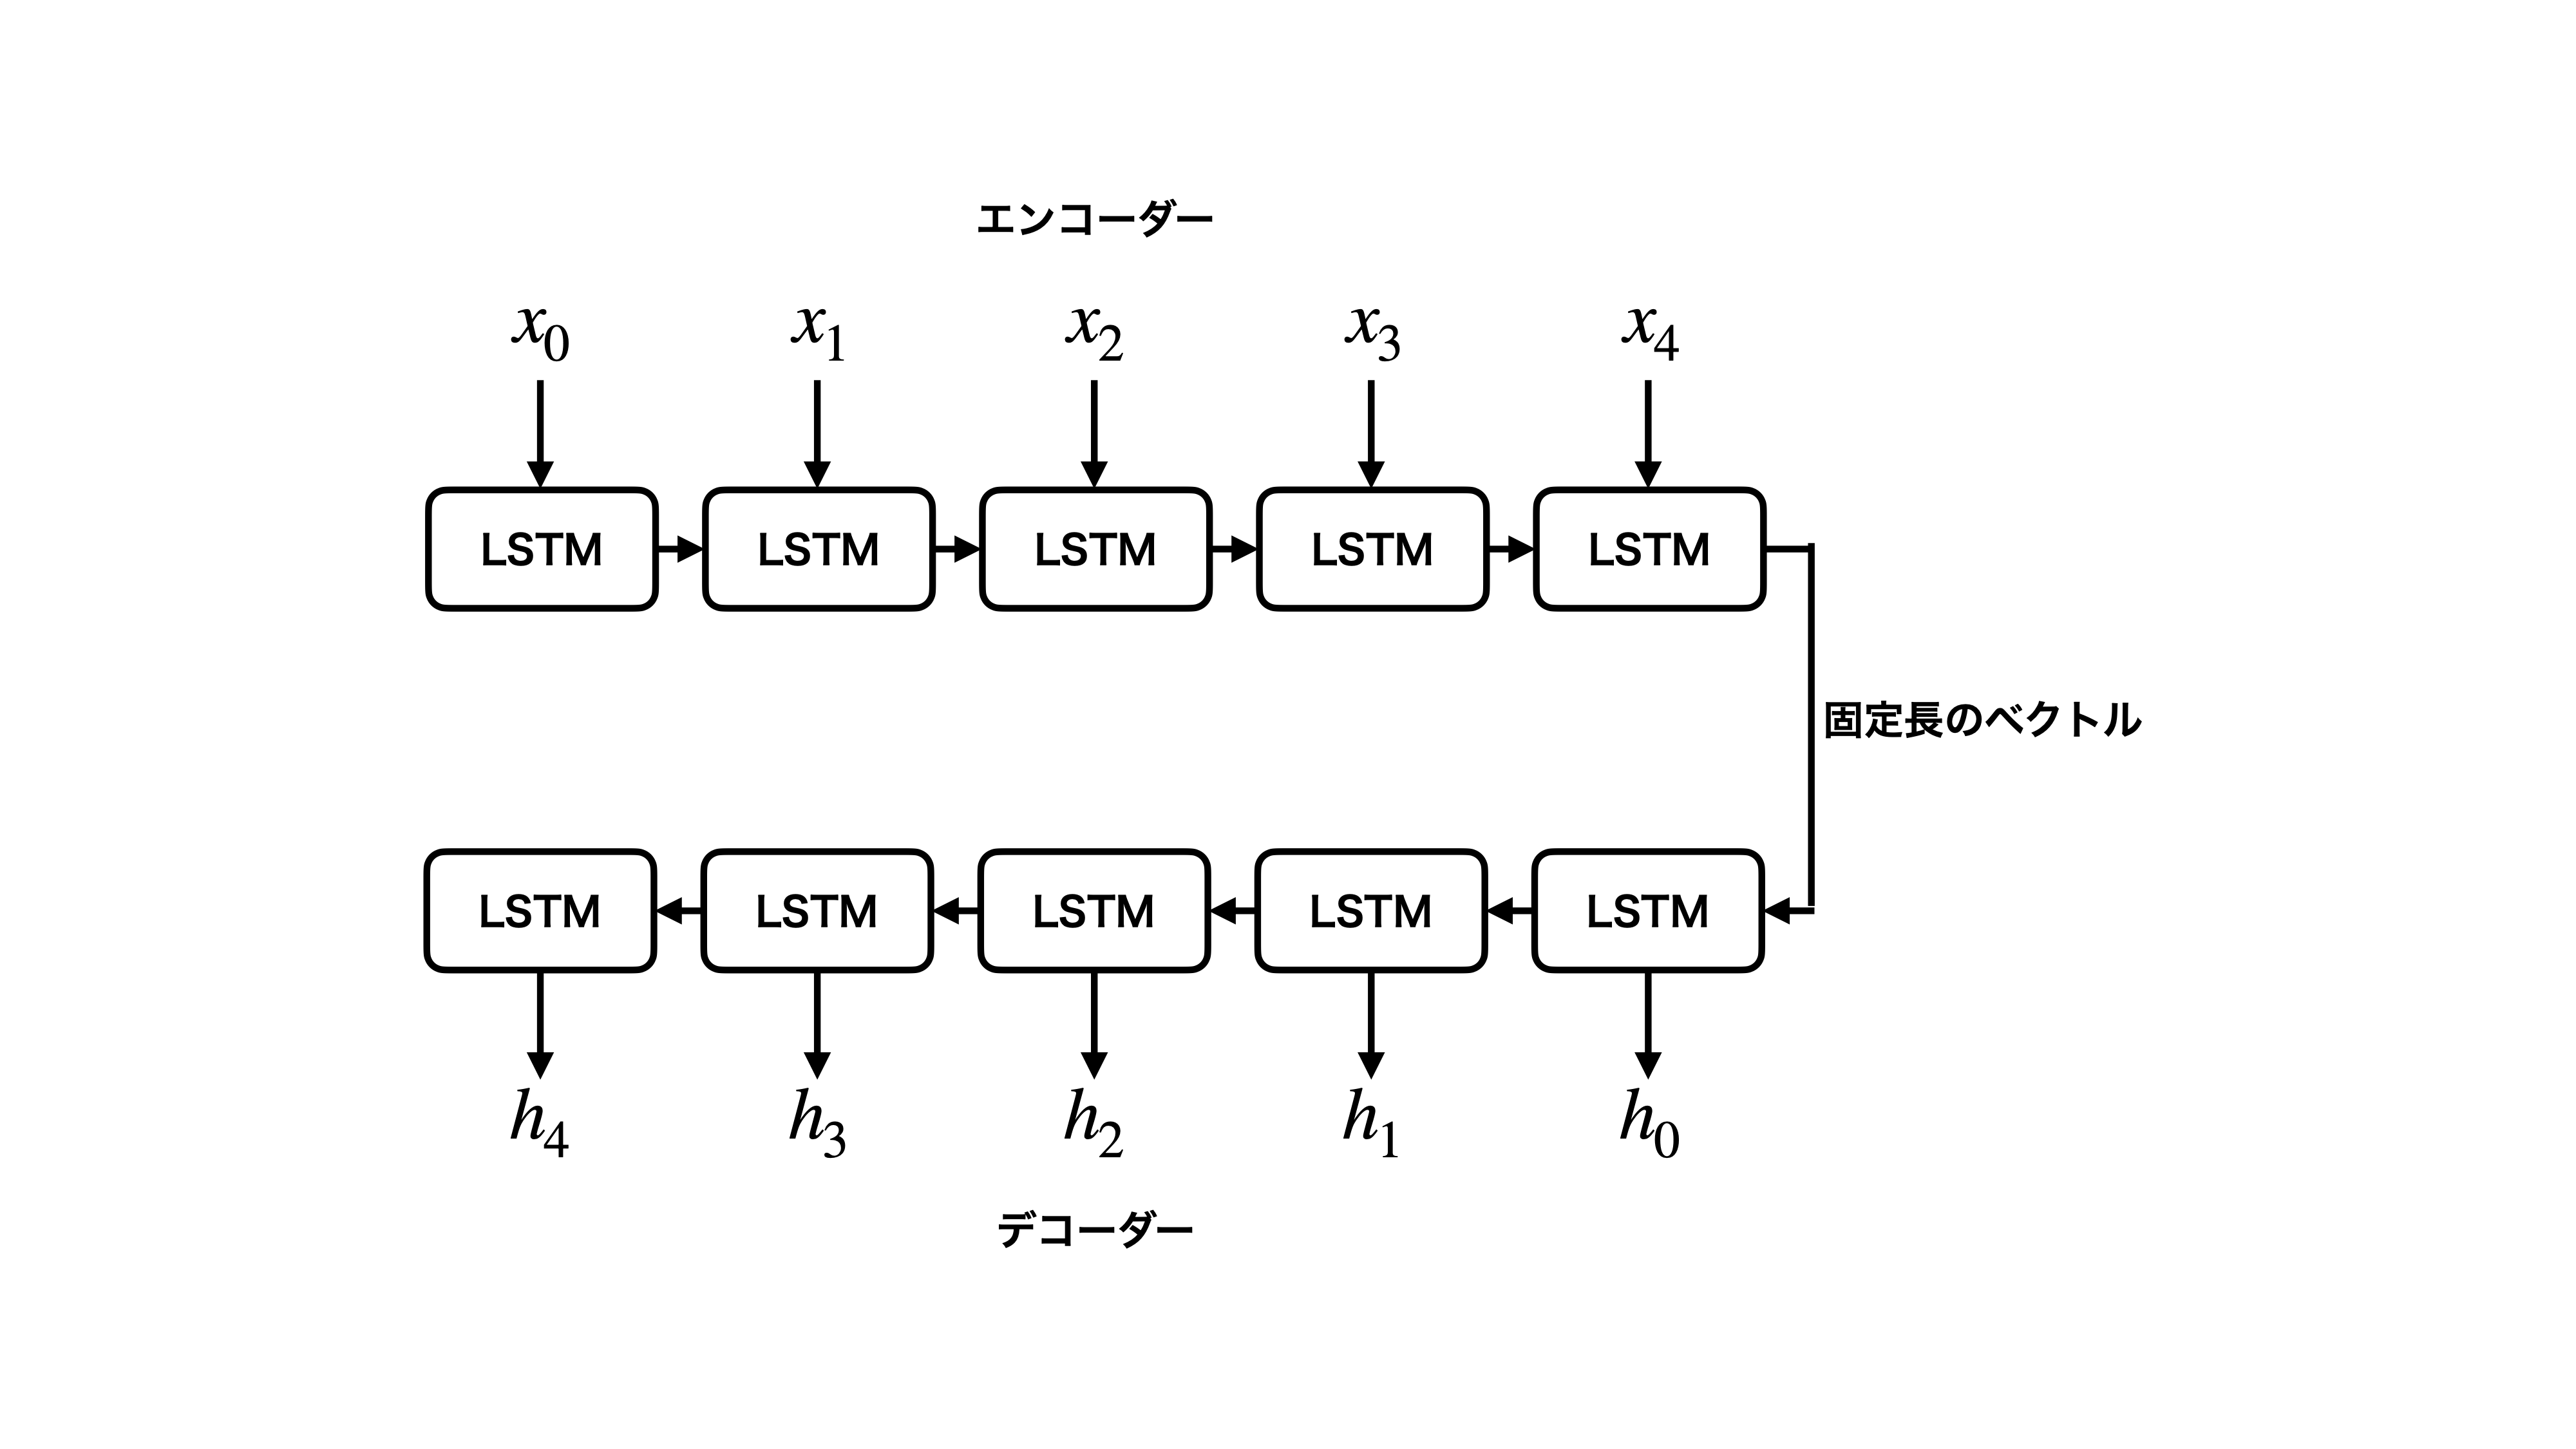
\includegraphics[trim = 100 100 100 200, width=1.0\textwidth, clip]{Figure/2DeepLearning/18EncoderDecoderLSTM.png}
 \caption[LSTMによるエンコーダー・デコーダーモデル]{LSTMによるエンコーダー・デコーダーモデル。図下部がエンコーダー部, 図上部がデコーダー部である。エンコーダー部の入力${\mbox{\boldmath{$x$}}}$から抽出された情報は図右の固定長のベクトルへと集約される。デコーダー部ではこの固定長のベクトルを初期状態にして出力${\mbox{\boldmath{$h$}}}$の生成を行う。}
 \label{18EncoderDecoderLSTM}
\end{figure}

この問題を解決するための技術がAttentionである。
Attentionを組み込んだLSTMのエンコーダー・デコーダーモデルを図\ref{19EncoderDecoderAttention}に示す。
ここで, 図中のAttentionと示している部分は, 実際にはエンコーダーの全ての系列の出力を集めた行列である。
このようにして, Attentionは系列長に依存した情報量を確保できる。
次項ではより詳細なAttentionの計算について説明する。

\begin{figure}[htbp]
 \centering
 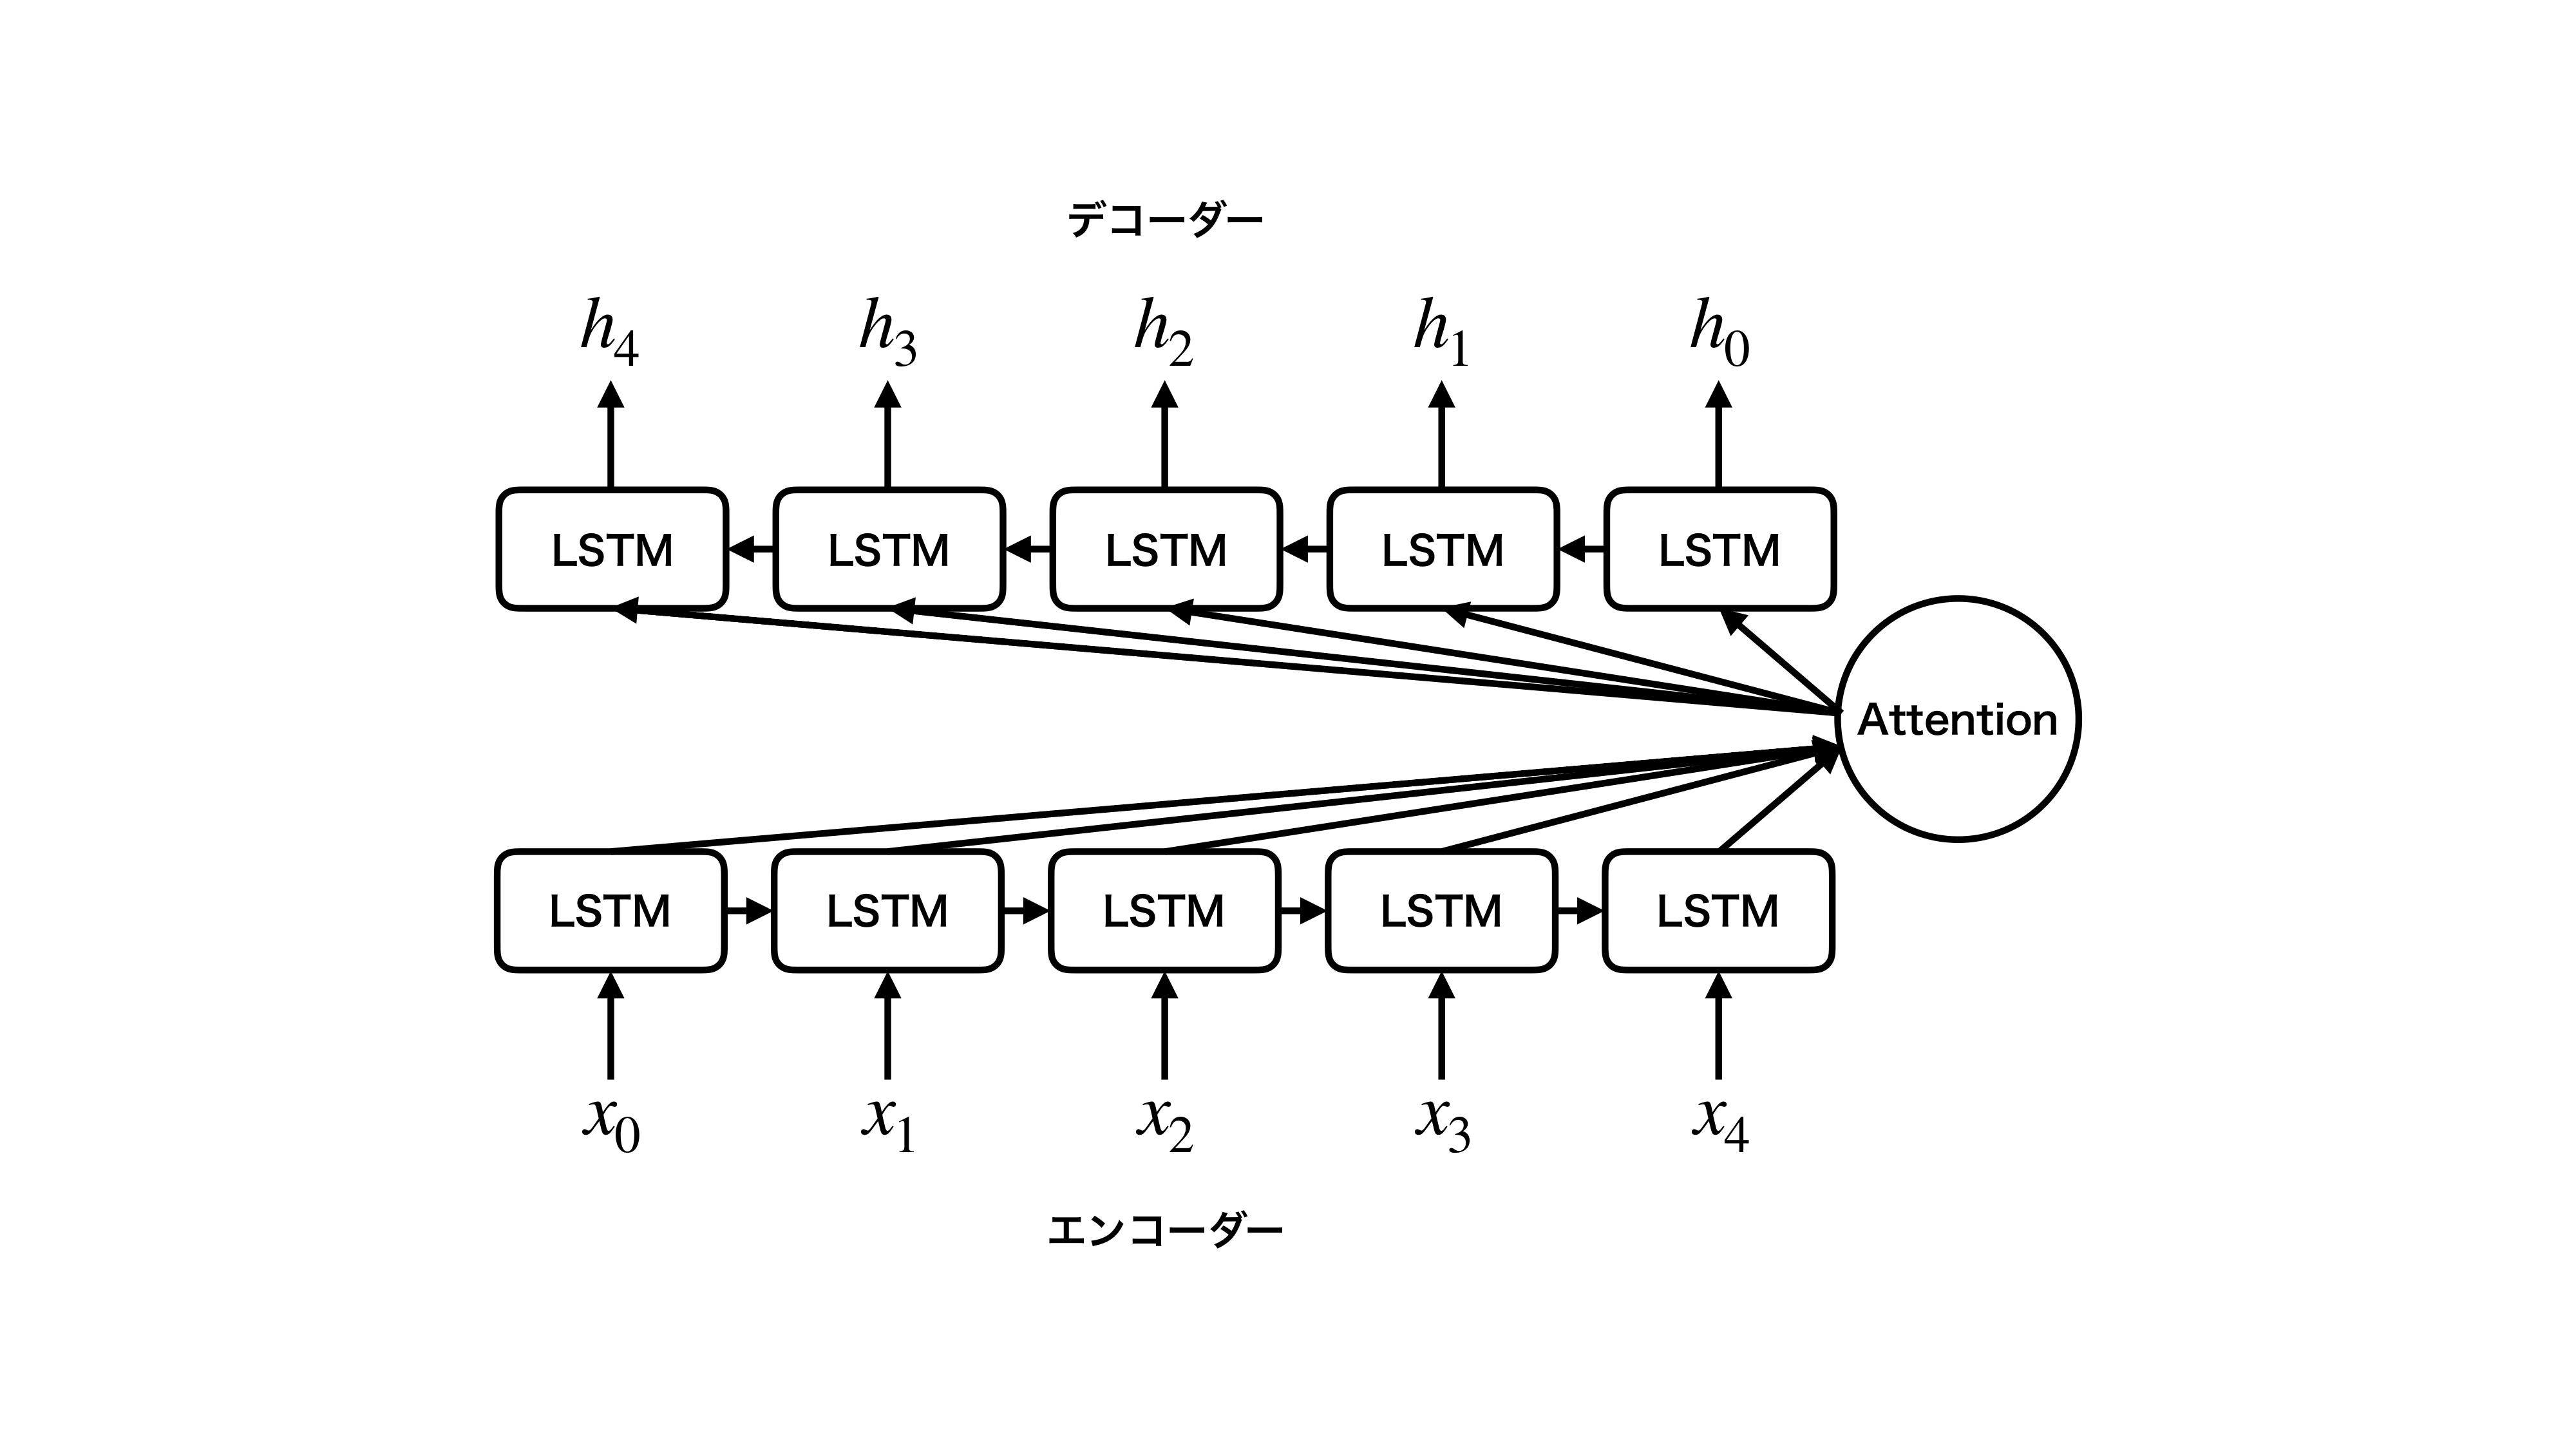
\includegraphics[trim = 100 100 100 200, width=1.0\textwidth, clip]{Figure/2DeepLearning/19EncoderDecoderAttention.png}
 \caption[AttentionとLSTMによるエンコーダー・デコーダーモデル]{AttentionとLSTMによるエンコーダー・デコーダーモデル。図下部がエンコーダー部, 図上部がデコーダー部である。エンコーダー部で抽出された情報は図右のAttentionに集約される。これは後述するKeyやValueに相当する。Attentionの大きさはエンコーダー部の入力系列長に依存しており, 常に適切な情報量を確保できる。}
 \label{19EncoderDecoderAttention}
\end{figure}


%%%%%%%%%%%%%%%%%%%%%%%%%%%%%%%%%%%%%%%%%%%%%%%%%%%%%%%%%%%%%%%%%%%%%%%%
\subsection{Attention} \label{DL:Atten:Attention}

図\ref{19EncoderDecoderAttention}では, エンコーダーとデコーダーの間にAttentionを表現しているが, 実際にはAttentionはデコーダーの個々の系列に応じて計算される。
これは, デコーダーのある系列$t$がエンコーダー全体のどの情報に注目しているかを逐次計算しなくてはならない為である。
Attentionの実装の仕方は多岐にわたるが, その計算は次のような手順にまとめられる。

\begin{enumerate}
  \item Query, Key, Valueを用意する。
  \item QueryとKeyを用いて, Attention Weightを計算する。
  \item Attention WeightとValueを用いて, コンテキストを作成する。
\end{enumerate}

Query, Key, Valueにおいて, KeyとValueは同じものが用いられることが多い。
KeyとValueは図\ref{19EncoderDecoderAttention}のエンコーダーの全ての系列の出力を集めた行列に相当している。
Queryとはここでは, デコーダーの個々の系列である$t-1$番目の出力 (隠れ状態) である。
したがって, QueryとKeyを用いて, Attention Weightを計算するという操作は$t-1$番目の隠れ状態 (Query) とエンコーダーの全ての系列の出力を集めた行列 (Key) を用いて, どこに注意するかを表現した重み (Attention Weight) を計算していることを意味している。
次に, このAttention Weightを, もう一度エンコーダーの全ての系列の出力を集めた行列 (Value) に掛けることで, エンコーダーのそれぞれの系列の情報を注意しながら取り出すことができる。
この取り出された情報をコンテキストといい, Attentionではこのコンテキストをデコーダー部に使用することで, 系列長に依存した情報量を保持している。

Attention Weightの計算方法はいくつかの手法が存在しているが, ここでは最も単純な手法を二つ述べる。
\begin{itemize}
  \item Additive Attention\cite{BahdanauAttention}\\
  Additive Attentionの利点はQueryとKeyがどのような大きさであっても計算できるという点である。
  N番目のQueryとKeyがそれぞれ, 大きさ[F]と[E, M]のベクトルと行列であるとすると, その計算は図\ref{20Attention}の上段ように表現できる。
  ここでN番目のQueryは系列長のM回分反復されており, 最終的に大きさ[F, M]の行列となっている。
  Additive Attentionの特徴はAttentionの内部に独自の学習可能な重みを保持している点である。
  N番目のQuery行列とKeyはそれぞれ重み行列と掛けられ, 得られたそれぞれの行列要素について和を取っている。
  その後, 更に大きさ[D]の重みベクトルと掛けられ, 大きさ[M]のエネルギー (図\ref{20Attention}中のベクトル e N) を得る。
  このベクトルについて, ソフトマックスと同様の関数で規格化し, Attention Weightを作成している。
  この計算はフィードフォワードニューラルネットワークそのものであり, Additive Attentionはこのように内部にネットワークを持っているため, 後述するDot-Product Attentionと比較して計算が遅くなるという欠点を抱えている。

  \item Dot-Product Attention\cite{LuongAttention}\\
  Dot-Product AttentionはAdditive Attentionと比較して非常にシンプルな構造をしている。
  その計算を図\ref{20Attention}の下段に示している。
  図からも分かるようにAdditive Attentionとは異なり, 内部に重みを保持しておらず, QueryとKeyから直接Attention Weightを計算している。
  ただし, このようにQueryとKeyを掛けるためには, それぞれの大きさを揃える必要があり, 具体的には$E=F$の時のみこのDot-Product Attentionを使用することができる。
\end{itemize}
  
\begin{figure}[htbp]
 \centering
 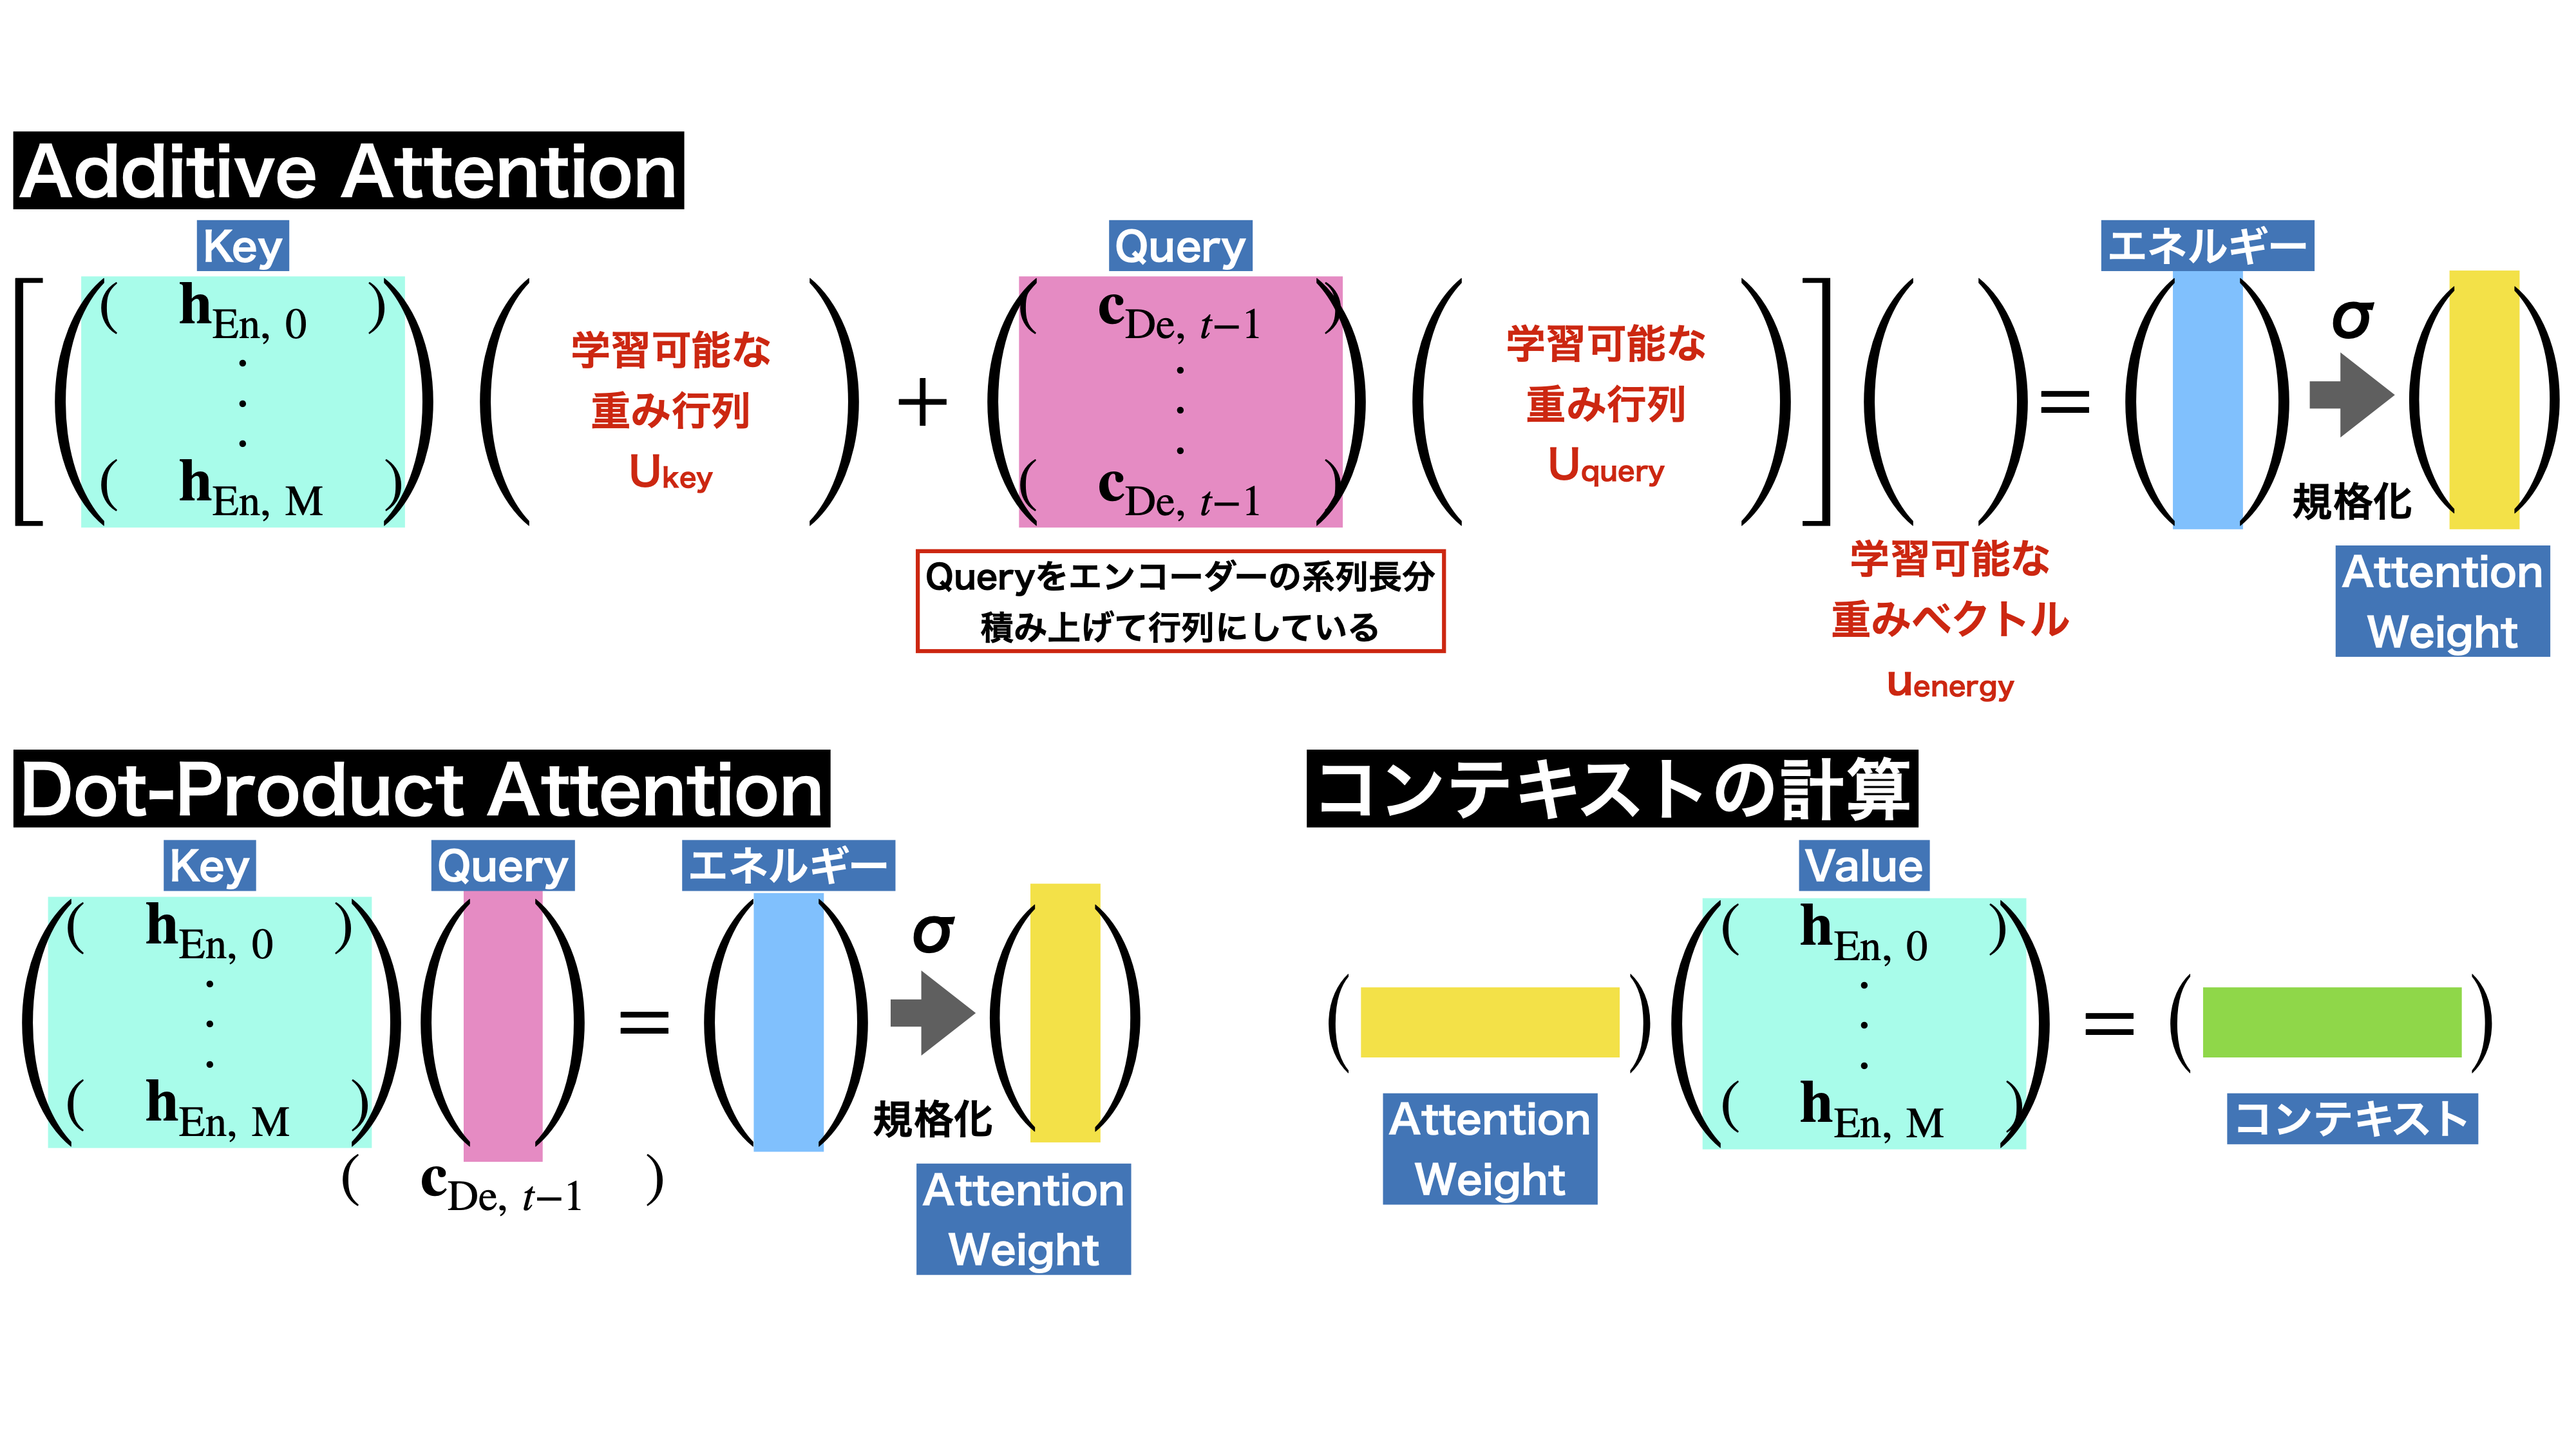
\includegraphics[trim = 200 100 200 100, width=1.0\textwidth, clip]{Figure/2DeepLearning/20Attention.png}
 \caption{Additive Attention と Dot-Product Attention}
 \label{20Attention}
\end{figure}

コンテキストをどのように以降の計算へ組み込むのかについての具体的な例は, 本研究の\ref{Net:VLSTM:StructureofVLSTM}項に示している。
上記のように計算されたAttention Weightを確認することでネットワークの理解をより深めることができる。
このAttention Weightはあるデコーダー部の$1$系列がエンコーダー部の全系列に対して何処に注意しているかを表現している事に再度注意しておく。
したがって, デコーダー部の全系列に対してAttention Weightを計算した場合, それは行がデコーダー部の系列長, 列がエンコーダー部の系列長の行列となる。
Attention Weightに関する具体的な図についても本研究の\ref{Net:VLSTM:PerformanceofVLSTM}項で確認する。

Attentionは"Attention is all you need\cite{AttentionIsAllYouNeed}"と言われるほど, 近年非常に注目されている技術である。
ここでは, AttentionをLSTMの補助として使用している例を挙げたが, Attentionは様々な技術と組み合わせられる。
またそれだけでなく, Attentionのみを用いて構成された, Transformerと呼ばれるモデルは2021年現在において, 自然言語処理の標準的なネットワークであると言われるほどの性能と, LSTMでは実現できなかった速さを両立している。


%%%%%%%%%%%%%%%%%%%%%%%%%%%%%%%%%%%%%%%%%%%%%%%%%%%%%%%%%%%%%%%%%%%%%%%%%%%%%%%%%%%%%%%%%%%%%%%%%%%%%
\section{ハイパーパラメータ} \label{DL:HyperParameter}

ここまでで述べたように深層学習は教師あり学習であるため, 訓練データを用いて重みの更新を行い, ネットワークの重み (パラメータ) を調整 (チューン) していく。
しかし, ネットワークはネットワーク自体を構築するための, 学習によって更新されないパラメータをいくつか持っている。
このようなパラメータをハイパーパラメータという。
ハイパーパラメータは学習前に設定しておく必要があり, ネットワークの性能を引き出すためには適切に最適化 (ハイパーパラメータ・チューニング) が必要がある。
ハイパーパラメータの種類や数はネットワークの構造によって大きく異なるが, 一般にチューニングが必要とされるハイパーパラメータについて以下に示す。

\begin{itemize}
  \item 最適化手法 (Optimizer) : RMSPropやAdamといった重み更新の為の最適化手法
  \item 学習率 (Learning rate) : 重み更新のステップ幅
  \item エポック数 (Epochs) : 学習回数・訓練データを一周学習することを1エポックという
  \item バッチサイズ (Batch size) : ミニバッチ学習における訓練データサンプルの大きさ
  \item ノード数 (Node) : 重み行列の大きさ
  \item 層の数 (Layer) : フィードフォワードネットワークにおける全結合層の数
\end{itemize}

これらはハイパーパラメータの一例であり, それぞれについて適切に選ぶ必要がある。
ハイパーパラメータの探索手法も幾つか提案されており, ランダムサーチやグリッドサーチ, ベイズ最適化などが用いられている。

以上が本論文のための深層学習の導入である。
この\ref{chap:DeepLearning}章を前提として, \ref{chap:Networks}章での本研究で使用したネットワークの構造を解説していく。
以降の章では, ここで挙げた深層学習の用語を説明せずに使用するが, その場合は適宜, 本章を参照していただきたい。
また, 本章の初めや\ref{DL:NeuralNetwork}でも述べたように, 深層学習の実装に関しては様々なフレームワークがあるため, ここでの記載は省かせていただく, 本研究の実装に関しては付録\ref{sec:Code}や私のGitHub\cite{GitHubGotoK}にまとめている。















